
\documentclass{thesis}

\subtitle{Diplomarbeit}
\title{Algorithmen zur automatisierten Generalisierung durch Zusammenfassung von Linienzügen in OpenStreetMap\\ für konkrete Spezialfälle}
\author{Arne Johannessen}
\publishers{betreut durch\\ Prof. Dr. rer. nat. Detlef Günther-Diringer\\ und\\ Dipl.-Wi.-Ing. Frederik Ramm}
%\date{Arbeitsentwurf}
%\dedication{}

\begin{document}

\maketitle

%\begin{abstract}
%\end{abstract}

\tableofcontents
\chapter{Einleitung}

\begin{itemize}
	\item erste, grobe Einführung ins Thema
	\item knapper Abriss des Kontextes der Fragestellung in Grundzügen (vgl. Themenblatt)
	\item was macht die Fragestellung interessant? (Motivation -- evtl. schon einzelne Anwendungsfälle umreißen)
	\item Gesamtüberblick der Arbeit einschließlich ihrer Ergebnisse, roter Faden als Orientierung für den Leser
	\item Eindruck an den Leser: warum soll er diese Arbeit weiterlesen oder welche Kapitel kann er überspringen
\end{itemize}

% UTF-8

\documentclass[../main/thesis.tex]{subfiles}
\onlyinsubfile{\setcounter{chapter}{1}}  % single-chapter command
%\onlyinsubfile{\renewcommand{\BibTeXenabled}{1}}
\begin{document}


\chapter{Analyse der Ausgangslage}

\section{OpenStreetMap: Alles für Alle}
\label{ch:osm-intro}

Ziel des Projekts OpenStreetMap (OSM) ist die Erstellung einer Geodatenbank für eine freie Weltkarte. \cf[47]{Top09}
Zehntausende Freiwillige verwenden z.~B. in ihrer Freizeit preisgünstige tragbare GPS-Empfänger oder dafür freigegebene Luftbilder, um Geodaten zu erfassen (\term{volunteered geographic information,} VGI). \cf[148--149, 154]{NZ12}
Die so erstellte Geodatenbank kann unter einer freien Lizenz%
\footnote{Seit 12.~September 2012 verwendet OSM die Open~Database~License (ODbL). \cf{osm:ODbL}}
zu beliebigen Zwecken weiterverwendet werden. \cf[119--120]{SP11}

%Im Unterschied zu kommerziell verfügbaren Geodaten anderer Anbieter (Ämter, Navteq etc.) entstehen bei \osm\ keine Lizenzkosten. \noref\
%Im Unterschied zu kostenlos verfügbaren Kartendarstellungen anderer Anbieter (Google, Ämter etc.) sind bei \osm\ auch die rohen Geodaten verfügbar und erlauben die ... \cf[6]{RT09}
%%Im Gegensatz zu vielen amtlichen Geobasisdaten dürfen OpenStreetMap-Daten lizenzkostenfrei verwendet werden, auch für kommerzielle Zwecke. \cf[217, 221\f]{RT09}
% \cf[336]{Böh07}
% [lgm05 3 (LG München, Beschl. vom 9. Nov. 2005, Az. 21 O 7402/02, 3; in: GRUR 2006, 225)]

Das von \osm\ verwendete Datenmodell ist sehr einfach gehalten:
Es kennt nur Punkte \term{(nodes),} Linienzüge \term{(ways)} und Relationen, die alle jeweils über Attribute \term{(tags)} in Form von \term{key-value-pairs}%
\footnote{\osm-\term{tags} sind Kombinationen aus zwei Zeichenketten: einem Attributschlüssel und einem Wert. \cf[52]{RT09} Sie werden meist als \osmtag{key}[value] notiert (z.\,B. \osmtag{name}[Geofabrik]).}
verfügen können.
Dabei definieren \term{ways} eine Liste von \term{nodes} als ihre Stützpunkte, während Relationen Beziehungen zwischen mehreren \term{ways,} \term{nodes} oder anderen Relationen ausdrücken.
Flächen werden nur über \term{tags} modelliert.
\cf[49--55]{RT09}

Der Name „OpenStreetMap“ mag irreführend sein, denn es handelt sich dabei nicht um eine Straßenkarte, sondern vielmehr um eine maßstabslose Datenbank mit teils sehr detaillierten Inhalten nahezu beliebiger Themen. \cf[115--116]{SP11}
Alle \osm-Attribute sind Freitext-Angaben ohne starre Klassifizierungsschemata oder Kartierschlüssel.
Syntax und Semantik der einzelnen \term{tags} werden seit der Gründung von \osm\ fortlaufend von den Beitragenden diskutiert, gestützt auf bisherige Erfahrungen.
Die Diskussion findet vornehmlich im Internet statt; Ergebnisse werden öffentlich dokumentiert und in Software wie z.~B. Renderern implementiert.
Wer neue Inhalte erfasst, orientiert sich oft an den bisher in der Datenbank üblichen oder im Web dokumentierten Konventionen. \cf[59--62]{RT09}

Dieses Vorgehen hat
%gegenüber einer vor der Erfassung vereinbarten gemeinsamen Ontologie \cf[14]{GOS09}
zur Folge, dass die zu OSM Beitragenden genau das erfassen, was sie persönlich für interessant oder wichtig halten. \cf[47--48]{Top09}
Jeder der Beitragenden entscheidet somit die Kriterien für die Erfassungsgeneralisierung jeweils für sich selbst.
\osm-Daten sind dadurch zwar inhomogen, verfügen aber oft über einen sehr hohen Detailreichtum. \cf{Sch12}
So könnten zum Beispiel für Teilstücke einer Straße \term{tags} für Tempolimits, Überholverbote, Fahrspurenanzahl, Oberflächenmaterial sowie -qualität, Baujahr und mehr eingetragen worden sein. \cf[115]{SP11}

% "alles für alle": Es können *alle* Datenthemen beliebig detailliert erfasst werden und stehen aufgrund der freien Lizenz dann *allen* Nutzern zur Verfügung => enormer Detailreichtum, aber auch u. U. enorme Schwierigkeiten, der Datenmengen Herr zu werden.

%Dies führt zu großen regionalen Unterschieden in Datendichte, -aktualität und -qualität.
%„Die individuelle Interessenlage des Nutzers ist [...] zugleich Stärke und Schwäche“ \citex[115]{SP11} von \osm.

Veränderungen an den Attributen im Verlauf eines \term{ways} führen im \osm-Datenmodell zwangsläufig zu einer Fragmentierung in mehrere aufeinander folgende \term{ways,} jeweils mit unterschiedlichen \term{tags.}
Dies erhöht die Datenmenge und erschwert die Weiterverarbeitung.
Eine Verknüpfung dieser Fragmente -- im aktuellen \osm-Datenmodell durch Relationen -- kann in manchem Kontext hilfreich sein, ist jedoch auch eine Quelle neuer Probleme. \cf[56--57]{RT09}
Es wäre außerdem möglich, einander parallele \term{ways} in gleicher Weise über Relationen zu verknüpfen, um das Zusammenfassen zu erleichtern.

Für Organisationen mit homogeneren Datenbeständen und Erfassungsweisen wie etwa Vermessungsämter wäre eine solche Lösung naheliegend.
So erfasst beispielsweise die deutsche Landesvermessung die Straßenachse bereits in den Basisdaten mitsamt Verknüpfungen zu allen Fahrbahnen und Fragmenten. \cf[48--50]{adv08a}
Einige Generalisierungsvorgänge werden so deutlich vereinfacht. \cf[193]{UD06}

In \osm\ ist dies jedoch bisher nicht üblich.
Tatsächlich scheinen Relationen vergleichsweise wenig Beachtung zu finden.%
\footnote{Neuere Forschung bestätigt dies jedenfalls allgemein und anekdotenhaft. \cf[2]{PM17}}
%Während die \osm-Datenbank derzeit etwa $10^9$ \term{nodes} und $10^8$ \term{ways} enthält, existieren nur etwa $10^6$ Relationen. \cf{osm:stats}
% "OpenStreetMap stats report run at 2013-03-18 00:00:04 +0000"
% Number of nodes      1816655618
% Number of ways       174204113
% Number of relations  1860585
%Weniger als $10^5$ Relationen weltweit sind mit dem Attribut \osmtag{route}[road] als Relationen gekennzeichnet, die \term{ways} einer Straße verknüpfen.%
%\footnote{Bis Fertigstellung der vorliegenden Arbeit hat sich die Anzahl der \osmtag{route}[road]--Relationen ungefähr verdoppelt auf etwa $130\,000$.}%
%\cf{osm:RouteRoad}
% 58712 relations with route=road
Möglicherweise hängt dies damit zusammen, dass Relationen von \osm-Software noch nicht optimal unterstützt werden. \cf[83]{RT09}

Das oben beschriebene Fehlen interner Strukturen unter den \osm"=Mitwirkenden (der Community) macht es aufwändig, die Erfassung und Kodierung der Geodaten zu verändern. \cf[84--85]{Sch09}
Änderungsvorschläge müssen zuerst von der Community akzeptiert und anschließend \emph{großräumig} und \emph{korrekt} in der Datenbank Anwendung finden.
Die Erfahrung zeigt, dass dies ein langwieriger Prozess sein kann.
Das macht eine automatisierte Ableitung der nötigen Informationen aus den bereits existierenden Geodaten interessant.



\section{Kartenherstellung mit OpenStreetMap} \label{kartenherstellung}

Wohl am bekanntesten ist OpenStreetMap für die auf der Projekt-Homepage \href{https://www.openstreetmap.org/}{\nolinkurl{osm.org}} zugängliche Web-Karte (Abbildung~\ref{fig:osm.org}).
Sie besteht aus quadratischen Kacheln \term{(tiles)} von $256\times\unit[256]{px}$, die dort in 19 verschiedenen Maßstäben%
\footnote{In 2013 wurde ein noch größerer, 20.~Maßstab ergänzt (bei null beginnend gezählt \cf{Dijk82} die Zoomstufe~19).}
von etwa $1 \nobreak : \nobreak 2000$ bis $1 \nobreak : \nobreak 500~\unit{Mio.}$ angeboten werden. \cf[154–155]{RT09}
Eine interaktive Oberfläche erlaubt über die freie Wahl der Zoomstufe eine Maßstabswahl und macht den Kartenausschnitt verschiebbar, so dass jeder im eingesetzten Kartennetz abbildbare Punkt der Erde angezeigt werden kann.
% evtl. Datenmenge etc. betonen

\onefigure{ht}{
	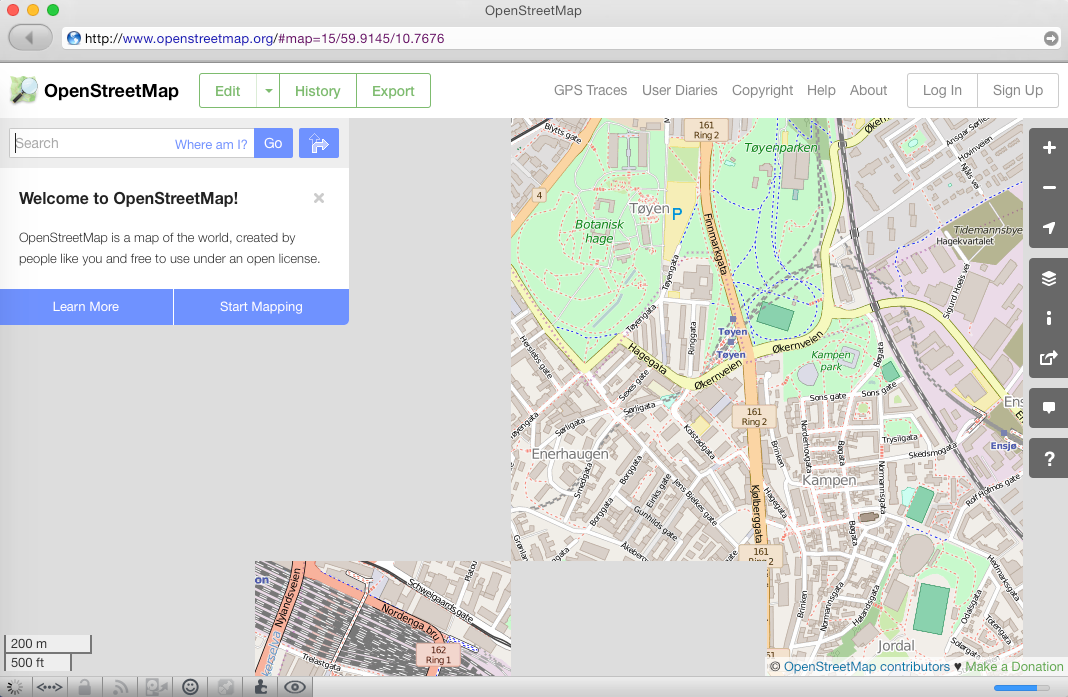
\includegraphics[width=\ScaleIfNeeded]{../chapter2/osm-org}
	\caption{Projekt-Homepage von OpenStreetMap während des Ladevorgangs}
	\label{fig:osm.org}
}

Wegen der sehr großen Anzahl von Kacheln werden diese in größeren Maßstäben \term{just in time} gezeichnet. \cf{osm:TileUsage}
Die Kartenbasis ist für alle Maßstäbe die jeweils minutengenau aktualisierte OSM-Datenbank.
%\noref % TODO: evtl. Verweis auf RT09, insb. für basis, minutengenau -> p. 157 zu osmarender, -> p. 195 zu diffs

Diese schnelle Aktualisierung ist für OpenStreetMap besonders wichtig, um den freiwillig Mitwirkenden nach einem Beitrag zur Datenbank ein schnelles Erfolgserlebnis zu geben, indem der Beitrag in der Karte weltweit für jeden sofort sichtbar wird.
Aus diesem Grund muss jede Generalisierung der Karte automatisiert ablaufen.
Weiterhin bedeutet die Zahl der Beiträge mit teilweise über 1000 \term{changesets} pro Stunde, \cf{Nei15}
% http://neis-one.org/2013/08/osm-activity-report-2013/
dass der Arbeitsaufwand für eine manuelle Generalisierung prohibitiv hoch wäre.
Klassische kartographische Generalisierung von Hand kommt daher nur für nicht nachzuführende und geographisch begrenzte Einzelanfertigungen in Betracht, etwa wenn auf Basis von OpenStreetMap eine traditionelle gedruckte Karte hergestellt werden soll.

Typischerweise besteht die Grundlage für Web-Karten wie derjenigen auf \url{osm.org} aus einer Geodatenbank, die mit einer Kopie der OpenStreetMap-Datenbank gefüllt und anschließend minütlich aktualisiert wird (Abbildung~\ref{fig:osm-datenfluss}).
Diese Geodatenbank enthält die Geometrie und Attribute \term{(tags)} der Rohdaten.
Vom Kartenleser in der interaktiven Oberfläche im Webbrowser erzeugte Anfragen nach Kacheln der Karte werden dann von der Renderer-Software unter Zugriff auf die Geodatenbank abgearbeitet, wobei die Geometrie anhand der vorgegebenen Zeichenregeln dargestellt wird.
Gerenderte Kacheln werden in einem Cache abgelegt und zum Browser geschickt.

Eigene Bearbeitungsschritte zur Generalisierung von Daten sind bei diesem Ablauf nicht vorgesehen (im Gegensatz zu den Abläufen im AAA-Modell der deutschen Landesvermessung  \cf[263]{ML12}).
Lediglich als Nebeneffekt des Einlesens in die Datenbank und des Zeichnens durch den Renderer wird eine begrenzte Modell-\noncf[194 17.2]{RT09} bzw. kartographische Generalisierung durchgeführt. \cf[194, 198]{RT09}
% http://wiki.openstreetmap.org/wiki/Mod_tile/Setup_of_your_own_tile_server

\onefigure{ht}{
	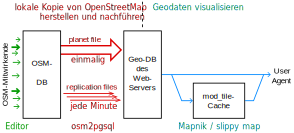
\includegraphics[width=\ScaleIfNeeded]{../chapter2/osm-datenfluss}
	\caption{typischer \osm-Datenfluss (vereinfacht dargestellt)}
	\label{fig:osm-datenfluss}
	% Mapnik nur ein Beispiel
}


% obiges trifft auf Linien, Punkte, Flächen gleichermaßen zu; hier darauf eingehen?


% LVAs verwenden (?) kartographische Hints, um die Ableitung von FOlge-DLMs zu erleichtern (?) [ML12, KN 62 (5) 263]. Das geht bei OSM nicht, weil auch das eben die Generalisierung und damit auch die Kartenherstellung verzögern und somit das schnelle ERfolgserlebnis verhindern würde. Es muss eben tatsächlich vollautomatisch ablaufen, wie auch immer.

% lesen: -> KN 56 (4) 191ff Modellgeneralisierung in ATKIS
% 193 (3.5): Kleeblatte sind "komplexes Objekt", d. h. leicht gesondert zu behandeln!


% MapCSS includes an eval function, and has rules that act as 'commands' to modify data. CartoCSS does not support eval or any data-modifying operations.
% https://gist.github.com/tmcw/4319642


% Angesichts dessen wären automatisiert abgeleitete, generalisierte Datenbanken für kleinere Maßstäbe zur Weiterverwendung wünschenswert, existieren jedoch bisher nicht. Entsprechend sind auch die aus OSM-Daten hergestellten Karten in aller Regel nicht kartographisch generalisiert: Nahe beieinander liegende Objekte überdecken einander scheinbar wahllos, Mindestgrößen und notwendige Formvereinfachungen werden von den automatischen Renderern ignoriert.

% Erschwert wird die Generalisierung von OSM-Daten unter anderem durch den hohen Grad der Fragmentierung von Linienzügen. Das Verknüpfen solcher zusammengehörenden, einzelnen ways durch Relationen in der Datenbank ist technisch möglich, wird aber von den Mitwirkenden aus unterschiedlichen Gründen nur sehr selten durchgeführt. Eine automatisierte Generalisierung durch Formvereinfachung (zur Reduktion der node-Anzahl) bedingt daher, dass die zusammengehörenden ways  dabei  als solche identifiziert werden. Gleiches gilt für die Generalisierung durch Zusammenfassung oder Verdrängung parallel verlaufender Linienzüge, beispielsweise Straßen mit begleitendem Radweg oder mehrgleisigen Bahnstrecken.



\section{Automatisierte Linien-Generalisierung von OpenStreetMap-Daten}
\label{ch:existing-generalisation}

Hake et~al. benennen sieben elementare Generalisierungsvorgänge:
„Vereinfachen -- Vergrößern -- Verdrängen -- Zusammenfassen [...] -- Auswählen [...] -- Klassifizieren -- Bewerten [...].“ \citex[168]{HGM02}
Von diesen lassen sich Auswahl (auf Basis der Objektklasse) sowie Vergrößerung und Bewertung (durch veränderte Strichbreite) vergleichsweise einfach im Renderer implementieren, da die Geometrie der zugrundeliegenden Geodaten dabei unverändert bleibt.

Andere Arten kartographischer Generalisierung wie etwa Formvereinfachung oder Zusammenfassung würden die Geometrie verändern, sind damit schwieriger zu implementieren und werden bisher nicht oder kaum eingesetzt.
Dies demonstrieren im Folgenden Beispiele zu einigen Generalisierungsvorgängen.



\subsection{Generalisierung durch Objektauswahl}

Zur Herstellung der Kacheln der Web-Karte wird für jede Zoomstufe eine Auswahl der jeweils darzustellenden Objektklassen vorgenommen.
Beispielsweise werden Anliegerstraßen \term{(residentials)} unterhalb von Zoom~12 nicht mehr dargestellt (Abbildungen~\ref{fig:kampen11} und~\ref{fig:kampen12}).
Dies vereinfacht das Kartenbild für den Betrachter und verringert die zu berechnende Datenmenge für den Renderer.

% Qualitätsumschlag fällt in OSM tlws. auch hierunter, gibt's aber nur für Flächen

\twofigures{ht}{
	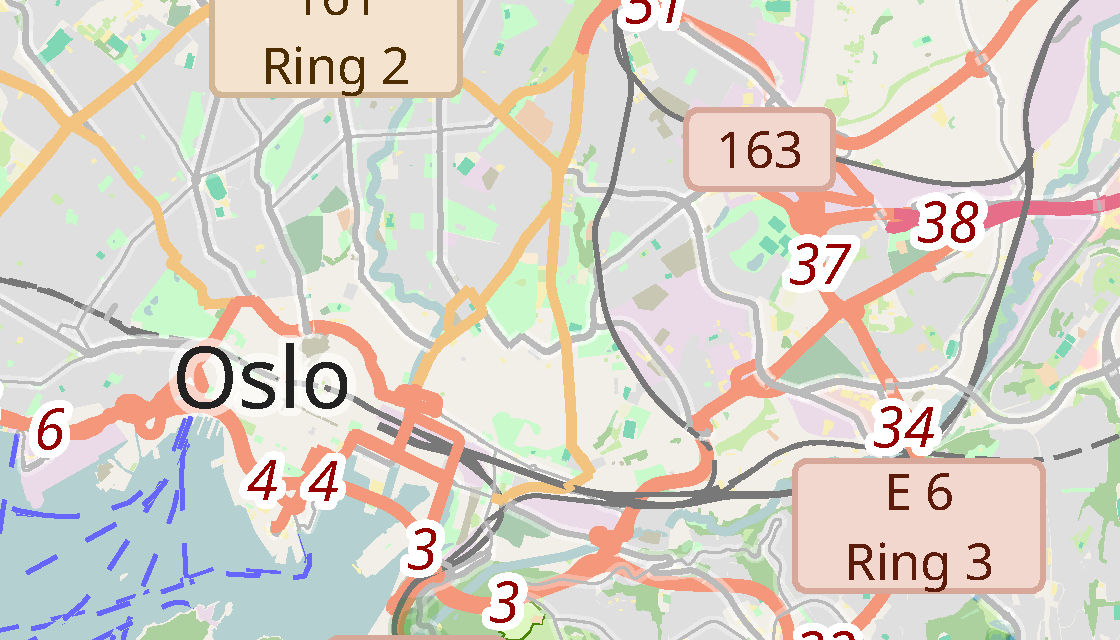
\includegraphics[width=\ScaleIfNeeded]{../chapter2/kampen-z11}
	\caption
		[Karte von \nolinkurl{osm.org}, Zoom~11, \term{residentials} nicht dargestellt]
		{Karte von \nolinkurl{osm.org}, Zoom~11, \term{residentials} nicht dargestellt \citex{map:osm-carto}}
	\label{fig:kampen11}
}{
	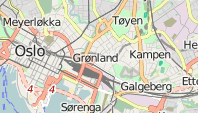
\includegraphics[width=\ScaleIfNeeded]{../chapter2/kampen-z12}
	\caption
		[Karte von \nolinkurl{osm.org}, Zoom~12, \term{residentials} dargestellt]
		{Karte von \nolinkurl{osm.org}, Zoom~12, \term{residentials} dargestellt \citex{map:osm-carto}}
	\label{fig:kampen12}
}



\subsection{Generalisierung durch Vergrößerung}
% Vergrößerung -> maßstabsbedingt notwendig

\twofigures{ht}{
	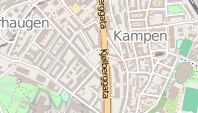
\includegraphics[width=\ScaleIfNeeded]{../chapter2/kampen-z14}
	\caption
		[Karte von \nolinkurl{osm.org}, Zoom~14, \term{residentials} 3~Pixel breit]
		{Karte von \nolinkurl{osm.org}, Zoom~14, \term{residentials} $\unit[3]{px}$ breit \citex{map:osm-carto}}
	\label{fig:kampen14}
}{
	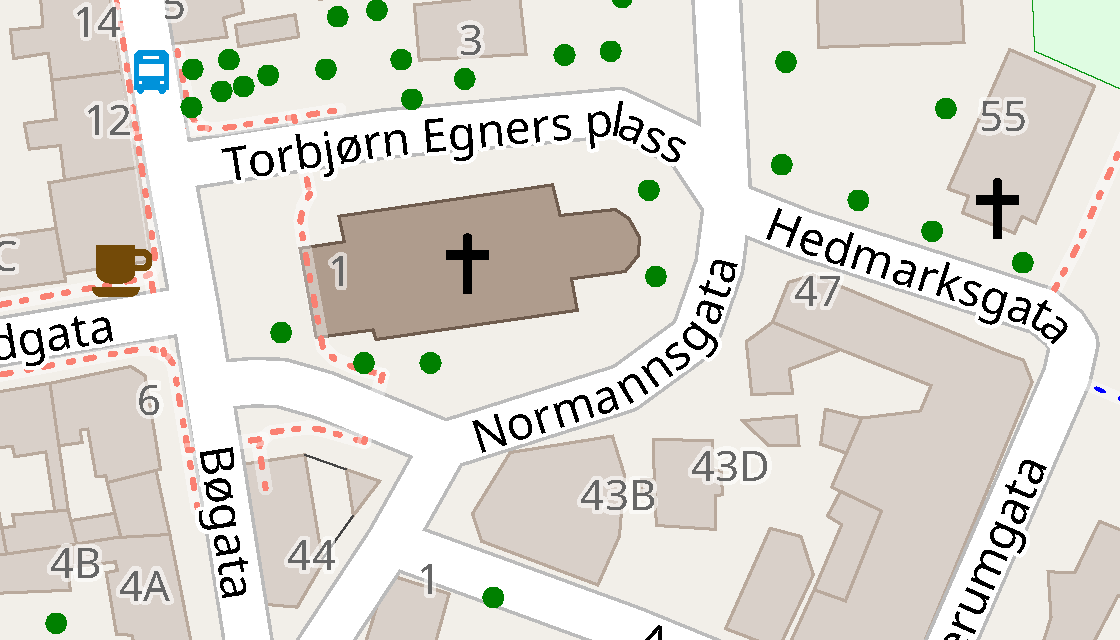
\includegraphics[width=7cm]{../chapter2/kampen-z17}
	\caption
		[Karte von \nolinkurl{osm.org}, Zoom~17, \term{residentials} 12~Pixel breit]
		{Karte von \nolinkurl{osm.org}, Zoom~17, \term{residentials} $\unit[12]{px}$ breit \citex{map:osm-carto}}
	\label{fig:kampen17}
}

\capstartfalse  % empty figures aren't supported by the document class
\twofigures{ht!}{
	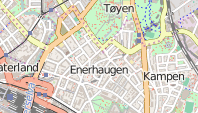
\includegraphics[width=\ScaleIfNeeded]{../chapter2/kampen-z13}
	\caption
		[Karte von \nolinkurl{osm.org}, Zoom~13, \term{residentials} 3~Pixel breit]
		{Karte von \nolinkurl{osm.org}, Zoom~13, \term{residentials} $\unit[3]{px}$ breit \citex{map:osm-carto}}
	\label{fig:kampen13}
}{
	\hspace{7cm}
}
\capstarttrue

Die Wahl der Zeichenregeln beinhaltet für einige Objektklassen auch eine Generalisierung durch Vergrößerung, indem für bestimmte Maßstäbe eine Strichbreite gewählt wird, welche im Abbildungsmaßstab die tatsächliche Größe des Objekts übersteigt.
Anliegerstraßen haben für die Zoomstufen 14 bis~19 jeweils eine unterschiedliche Strichbreite von $\unit[3]{px}$ bis $\unit[17]{px}$ definiert, so dass die Darstellung der Straße in der Karte Maßstabsänderungen andeutungsweise folgt (Abbildungen~\ref{fig:kampen14} und~\ref{fig:kampen17}). \cf{All15}
Die Breite von $\unit[3]{px}$ auf Zoom~14 entspräche ca.~$\unit[27]{m}$ in der Realität. \cf[155]{RT09}
Auf Zoom~13 werden Anliegerstraßen gar auf dieselbe Breite von $\unit[3]{px}$ gezeichnet (ca.~$\unit[57]{m}$) und damit deutlich vergrößert, um die Erkennbarkeit im kleinerem Maßstab zu fördern (Abbildungen~\ref{fig:kampen14} und~\ref{fig:kampen13}).

% z13+z14 erst 2015 exakt gleiche Strichbreite:
% https://github.com/gravitystorm/openstreetmap-carto/blob/fe4f8d48757cf85bb692129b5d9755ba5cadbbee/roads.mss
%@residential-width-z13:           3;
%@residential-width-z14:           3;
%@residential-width-z15:           5;
%@residential-width-z16:           6;
%@residential-width-z17:          12;
%@residential-width-z18:          14;
%@residential-width-z19:          21;



\subsection{Generalisierung durch Bewertung}
% Bewertung -> nach Bedeutung für den Kartenzweck

Weiterhin wird durch die Wahl der Zeichenregeln eine Bewertung der tatsächlich dargestellten Objekte vorgenommen, auch dies abhängig vom Maßstab.
So werden Anliegerstraßen auf Zoom~12 als schmaler, einfacher Strich gezeichnet, ab Zoom~13 jedoch als weißer Breitstrich mit grauem Rand (Abbildungen~\ref{fig:kampen12} und~\ref{fig:kampen13}).

% weitere Fälle von Bewertung: evtl. Klassifizierung nach primary, secondary etc mit unterschiedlich definierten Strichbreiten? TODO: verifizieren

%Ein unklares Kartenbild ist jedoch auch in weniger exotischen
% "näher liegenden"?
%Konstellationen zu beobachten. Ein weit verbreitetes Problem ist beispielsweise
%In vielen Fällen lässt sich allerdings ein unklares Kartenbild

\label{dual-highway-case-1}

Ein weit verbreitetes unklares Kartenbild lässt sich allerdings als scheinbare Betonung einiger auf \url{osm.org} gezeichneten Straßen missverstehen, wie Abbildung~\ref{fig:utrecht14} beispielhaft zeigt.
Die als Sammelstraße klassifizierte Croeselaan (bei Markierung~\textfiguremark{1}) wird mit breiterem Strich gezeichnet als Teile der Hauptstraßen (bei~\textfiguremark{2}).
Grund dafür sind nicht tatsächliche Unterschiede im Ausbauzustand%
\footnote{Der kürzlich begonnene in der Abbildung bei~\textfiguremark{2} zu erkennende Neubau einer Busfahrbahn verschmälert die Hauptstraße nicht.}
oder der Verkehrsbedeutung, sondern der Umstand, dass die Fahrbahnen der niederrangigen Straße durch einen breiten, parkähnlichen Grünstreifen getrennt werden  (Abbildung~\ref{fig:utrecht16}).
In kleinerem Maßstab überlappen sich die verbreitert gezeichneten Signaturen der beiden Fahrbahnen und fließen zusammen, so dass sich für den Betrachter der irreführende Eindruck einer besonders breiten oder wichtigen Straße ergibt.

Gleiches gilt für die ebenfalls in Abbildung~\ref{fig:utrecht14} auffallende wechselhafte Strichbreite einer Hauptstraße:
Hier existiert bei Markierung~\textfiguremark{2} nur eine einzige Fahrbahn, während sich bei~\textfiguremark{3} die Signaturen von zwei parallelen Fahrbahnen überlappen.

\twofigures{ht}{
	\begin{overpic}[width=\ScaleIfNeeded]{../chapter2/utrecht-z14}
		\put(115,48){\figureframe{.25}}
		\put(121,54){\figuremark[white]{1}}
		\put(30,45){\figuremark[white]{2}}
		\put(19,94){\figuremark[white]{3}}
	\end{overpic}
	% http://render.openstreetmap.org/cgi-bin/export?bbox=5.099716,52.074811,5.122461,52.082776&scale=30000&format=pdf
	\caption
		[Karte von \nolinkurl{osm.org}, Zoom~14, Zusammenfließen benachbarter Fahrbahnen]
		{Karte von \nolinkurl{osm.org}, Zoom~14, Zusammenfließen von benachbarten Fahrbahnen \citex{map:osm-carto}}
	\label{fig:utrecht14}
}{
	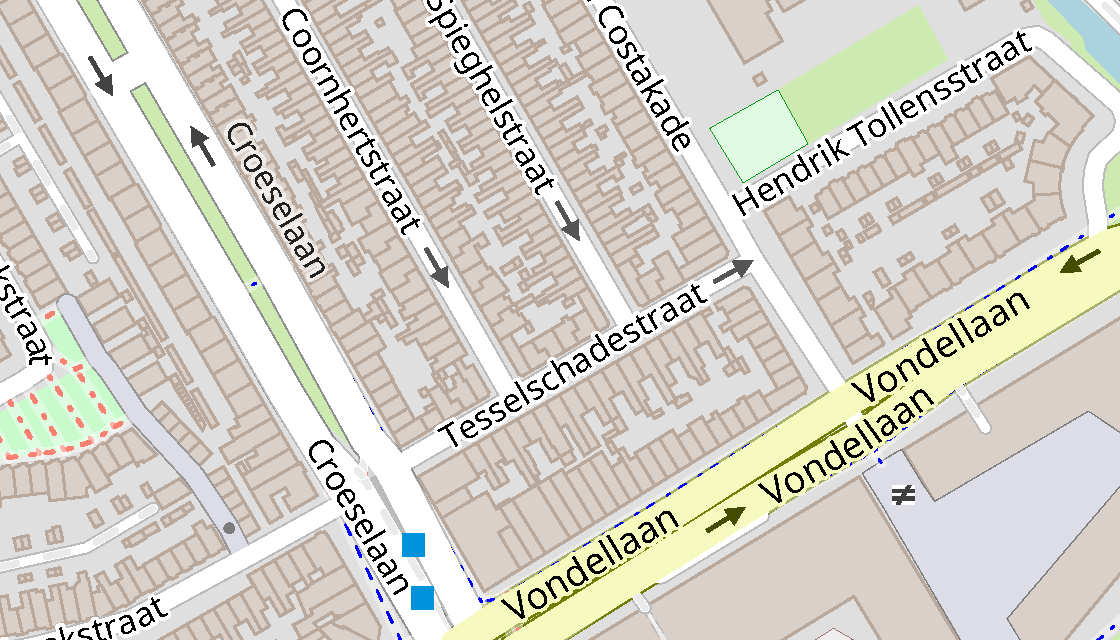
\includegraphics[width=\ScaleIfNeeded]{../chapter2/utrecht-z16}
	% http://render.openstreetmap.org/cgi-bin/export?bbox=5.112805,52.078108,5.118492,52.080099&scale=7500&format=pdf
	\caption
		[Karte von \nolinkurl{osm.org}, Zoom~16, Fahrbahnen getrennt erkennbar]
		{Karte von \nolinkurl{osm.org}, Zoom~16, Fahrbahnen getrennt erkennbar (\textfiguremark{1} in Abb.~\ref{fig:utrecht14}) \citex{map:osm-carto}}
	\label{fig:utrecht16}
}

Abbildung~\ref{fig:gera13} zeigt ein ähnlich unklares Kartenbild.
Hier ist die Hauptstraße längs der Eisenbahnstrecke bei Markierung~\textfiguremark{1} deutlich breiter als bei \textfiguremark{2}.
Auch hier liegt keine gezielte Bewertung vor; vielmehr wird die Straße von der Bahnstrecke teilweise verdeckt, so dass die Karte den falschen Eindruck einer unterschiedlichen Strichbreite verschafft.
Die eigentlich notwendige Verdrängung findet nicht statt.

\twofigures{ht}{
	\begin{overpic}[width=\ScaleIfNeeded]{../chapter2/gera-z13}
		\put(52,54){\figuremark[white]{1}}
		\put(64,77){\figuremark[white]{2}}
%		\put(23,44){\figureframe{.5}}
%		\put(118,96){\figuremark[white]{3}}
	\end{overpic}
	% http://render.openstreetmap.org/cgi-bin/export?bbox=12.058353,50.868971,12.102371,50.884842&scale=70000&format=pdf
	\caption
		[Karte von \nolinkurl{osm.org}, Zoom~13, Straße teilweise durch Bahnstrecke verdeckt]
		{Karte von \nolinkurl{osm.org}, Zoom~13, Straße teilweise durch Bahnstrecke verdeckt \citex{map:osm-carto}}
	\label{fig:gera13}
}{
	\begin{overpic}[width=\ScaleIfNeeded]{../chapter2/gera-z14}
		\put(65,21){\figuremark[white]{1}}
		\put(82,57){\figuremark[white]{2}}
	\end{overpic}
	% http://render.openstreetmap.org/cgi-bin/export?bbox=12.063503,50.875014,12.085512,50.88295&scale=35000&format=pdf
	\caption
		[Karte von \nolinkurl{osm.org}, Zoom~14, Straße neben Bahnstrecke]
		{Karte von \nolinkurl{osm.org}, Zoom~14, Straße neben Bahnstrecke \citex{map:osm-carto}}
%		{Karte von \nolinkurl{osm.org}, Zoom~14, Straße neben Bahnstrecke (\textfiguremark{3}~in Abbildung~\ref{fig:gera13}) \citex{map:osm-carto}}
	\label{fig:gera14}
}

Interessanterweise kehrt sich in größerem Maßstab das Verhältnis der Strichbreiten um:
In Abbildung~\ref{fig:gera14} ist die Hauptstraße bei Markierung~\textfiguremark{1} nun deutlich \emph{schmaler} als bei~\textfiguremark{2}.
Dies liegt an getrennt erfassten Richtungsfahrbahnen bei~\textfiguremark{2}, wie sie schon in Abbildung~\ref{fig:utrecht16} gezeigt wurden, während bei~\textfiguremark{1} mangels baulicher Trennung der beiden Fahrtrichtungen nur ein einziger Linienzug erfasst ist.
Wiederum handelt es sich nicht um eine gezielte Bewertung; der Anschein unterschiedlicher Strichbreiten ist unbeabsichtigt.



%\FloatBarrier
\subsection{Generalisierung durch Formvereinfachung}

Eine kartographische Formvereinfachung wird für die Web-Karte nicht vorgenommen.
Zufriedenstellende, voll automatisiert arbeitende Algorithmen dafür stehen nicht zur Verfügung und ein Eingreifen von Hand ist wie zuvor in Abschnitt \ref{kartenherstellung} erläutert nicht vorgesehen. \cf[25]{Kla11}
In kleineren Maßstäben ergibt dies beispielsweise für Straßen mit vielen kleineren Kurven eine zittrige Darstellung, so etwa in Abbildung~\ref{fig:trollstigen-osm} bei Markierung~\textfiguremark{1}.
Der Leser kann mit etwas Phantasie zwar erkennen, dass die Straße nicht absolut gerade verläuft, jedoch macht dies die Darstellung undeutlich und ist auch in diesem Maßstab nicht von Bedeutung.

\twofigures{ht}{
	\begin{overpic}[width=\ScaleIfNeeded]{../chapter2/trollstigen-z11}
		\put(87,16){\figuremark[white]{1}}
		\put(125,52){\figuremark[white]{2}}
	\end{overpic}
	\caption
		[Trollstigen, Web-Karte mit \osm-Daten, $1\nobreak:\nobreak135\,000$]
		{Trollstigen, Web-Karte mit \osm-Daten, $1\nobreak:\nobreak135\,000$ \citex{map:thunderforest}}
	\label{fig:trollstigen-osm}
}{
	\begin{overpic}[width=7cm]{../chapter2/trollstigen-kartverket-z11}
		\put(87,16){\figuremark[white]{1}}
		\put(125,52){\figuremark[white]{2}}
	\end{overpic}
	% replace Kartverket placeholder with custom-made example?
	% this example may be at a different scale than the OSM image!
	\caption
		[Trollstigen, manuell kartographisch generalisiert, $1\nobreak:\nobreak135\,000$]
		{Trollstigen, manuell kartographisch generalisiert, $1\nobreak:\nobreak135\,000$ \citex{map:n250}}
	\label{fig:trollstigen-manual}
}

An Serpentinen fällt dieser Mangel an Generalisierung besonders auf (Markierung~\textfiguremark{2}).
Im Extremfall kann sich hier in kleinem Maßstab durch das Zusammenfließen der Strecken zwischen den Kehren der falsche Eindruck einer großen, ebenen Straßenfläche ergeben (Abbildung~\ref{fig:trollstigen-osm}).
Eine sorgfältige Formvereinfachung müsste dagegen den Charakter der Straße durch Darstellung nur einiger ausgewählter Kehren mit vereinfachtem Verlauf erhalten (Abbildung~\ref{fig:trollstigen-manual}).
%Die Abbildungen~\ref{fig:trollstigen-osm} und~\ref{fig:trollstigen-manual} zeigen auch, wie in der kartographischen Generalisierung die Serpentinen als das Signifikante dieser Straße betont und die unwesentlichen kleineren Kurven davor und danach durch Formvereinfachung entfallen.

„Die Formvereinfachung ist insgesamt eine Reduzierung der Anzahl von Stützpunkten, wenngleich u.~U. lokal Stützpunkte hinzugefügt werden, um typische Formen übertreibend zu betonen.“ \citex[Formv.]{BK01}
Während Letzteres nach Kenntnis des Verfassers gegenwärtig nicht automatisiert möglich ist, kann eine bloße Reduzierung der Zahl der Stützpunkte zur Linienglättung automatisiert erfolgen.
Ein wichtiger Nebeneffekt ist dabei die verringerte Menge an Geodaten und damit deren vereinfachte Verarbeitung.
Der vielfach benutzte Algorithmus von Ramer, Douglas und Peucker zur Linienglättung zielt gerade auf Effizienz ab („efficient representation“ \citex[244]{Ram72}).
Eine Formvereinfachung nach kartographischen Gesichtspunkten ergibt sich mit ihm in der Regel nicht.

\onefigure{!b}{
	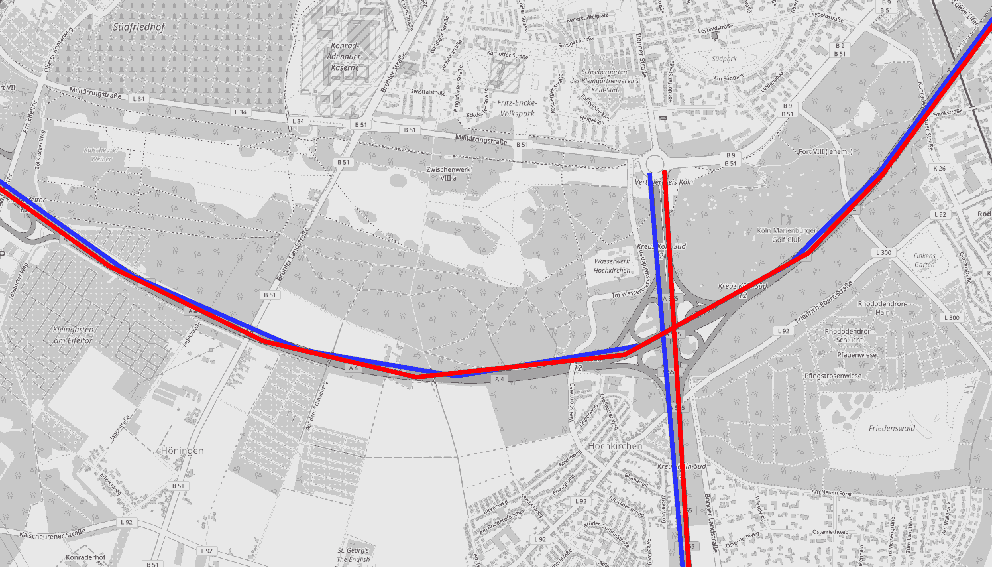
\includegraphics[width=12.25cm]{../chapter2/crossing}
	\caption
		[Überkreuzen paralleler Linienzüge nach Vereinfachung mit Ramer-Doug\-las-Peucker]
		{Überkreuzen paralleler Linienzüge nach Vereinfachung mit Ramer-Douglas-Peucker \citex[entsättigt][Hintergrund]{map:osm-carto}}
	\label{fig:crossing-parallels}
}
% TODO: Grafik neu erstellen: Originalkarte -> PSD -> Image/Adjustments/Black&White + QGIS-Export zur Registrierung => PDF in AI

Eines der Probleme bei der Automatisierung der Formvereinfachung besteht in der Notwendigkeit, alle vereinfachten Linien aufeinander abzustimmen, damit die charakteristischen Formen im Kartenbild insgesamt erhalten bleiben. \cf[\ibidabbr]{BK01}
%Formvereinfachung in kartographisch relevantem Ausmaß wäre daher nur mit einem ganzheitlichem Ansatz sinnvoll, der alle Objektklassen berücksichtigt und sie zueinander passend generalisiert.
%Beispielsweise müsste der Verlauf einer in einem engen Flusstal verlaufenden Straße in gleicher Weise vereinfacht werden wie der Verlauf des Flusses.
%Wenn nötig, müsste eines dieser beiden Objekte dazu auch verdrängt werden.
%Ein derart aufwändiger Vorgang wird nicht von dem für die Web-Karte genutzten Renderer Mapnik implementiert.
%Es wäre ein separater vorgeschalteter Schritt notwendig, welcher aus der lokalen ungeneralisierten Geodatenbank eine separate generalisierte Geodatenbank erzeugt, die dann von Mapnik gerendert werden könnte.
%Dies ist derzeit nicht der Fall.
Dies wird unter anderem dort deutlich, wo parallele Linienzüge mit Ramer-Douglas-Peucker vereinfacht werden.
%Optisch besonders auf{\nolig}fällig ist fehlende Erkennung paralleler Linienzüge als zusammengehörig, wenn sie einer starken Formvereinfachung unterzogen werden.
%Weil beide Linien dann unabhängig voneinander generalisiert werden, kann es abhängig vom eingesetzten Algorithmus zu unterschiedlichen Formen der beiden Linien kommen, die sich im Extremfall sogar gegenseitig überkreuzen können (Abbildung~\ref{fig:crossing-parallels}).

Beispielsweise zeigt Abbildung~\ref{fig:crossing-parallels} Richtungsfahrbahnen von Autobahnen, die nach Vereinfachung mit Ramer-Douglas-Peucker durch die ungleichmäßige Verteilung ihrer Stützpunkte stark variierende Abstände zueinander haben und sich sogar teilweise überkreuzen.
Dieses Problem ließe sich wenigstens für den Fall paralleler Linien leicht umgehen, wenn diese vor der Formvereinfachung zusammengefasst werden könnten.

Als weiteres Beispiel sind breite Flüsse zu nennen, für die in OpenStreetMap üblicherweise neben einer Mittellinie auch beide Uferlinien erfasst sind, um die flächenhafte Ausdehnung abzubilden.
Je nach den gewählten Parametern kann eine Formvereinfachung hier dazu führen, dass die Mittellinie das Flussbett verlässt. \cf[57]{Kla11}



%\FloatBarrier
\subsection{Generalisierung durch Verdrängung}

Typisch für Web-Karten ist das völlige Fehlen von Verdrängungen zur Einhaltung kartographischer Minimalabstände und -dimensionen.
Statt dessen werden mit kleiner werdendem Maßstab Objekte dichter und dichter aneinander, schließlich gar übereinander gezeichnet, worunter das Kartenbild teils erheblich leidet (Abbildung~\ref{fig:verdraengung}).
Web-Karten mit \osm-Daten sind hier keine Ausnahme.

\onefigure{ht}{
	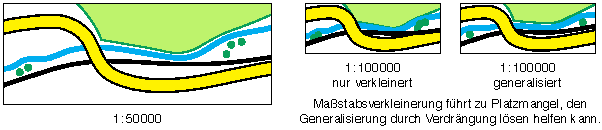
\includegraphics[width=13cm]{../chapter2/verdraengung}
	\caption
		[typisches Generalisierungsergebnis in Web-Karten]
		{typisches Generalisierungsergebnis in Web-Karten \cf[49]{sgk02}}
	\label{fig:verdraengung}
}

\twofigures{H}{
	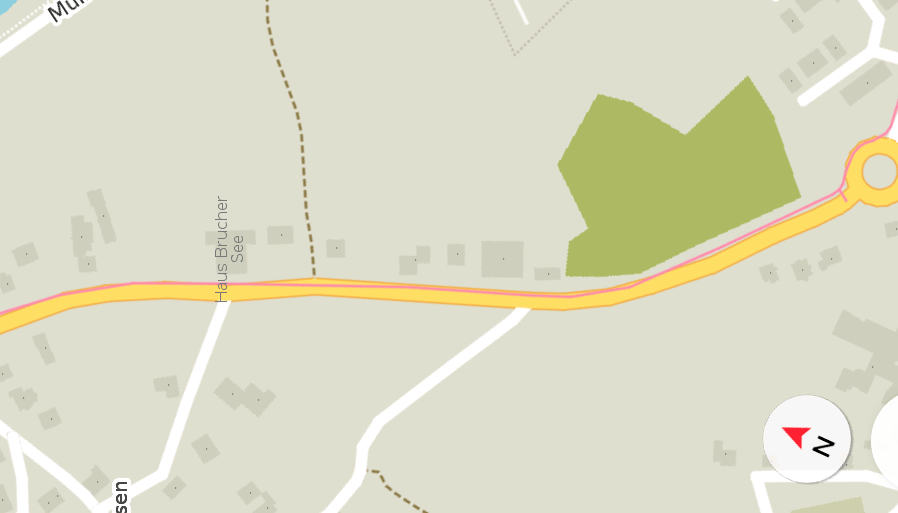
\includegraphics[width=\ScaleIfNeeded]{../chapter2/stuelinghausen-me}
	\caption
		[straßenbegleitender Radweg schneidet Straßenfläche]
		{straßenbegleitender Radweg (rot) schneidet Straßenfläche \citex[rotiert]{map:me}}
	\label{fig:stuelinghausen-maps.me}
	% Section 4 of the Apache License 2.0 used by maps.me permits relicensing of Derivative Works under different terms. It's not clear if this screenshot even qualifies as a Derivative Works under § 51 UrhG, but even if it does, relicensing under CC terms would be allowed as per the Apache License's terms.
}{
	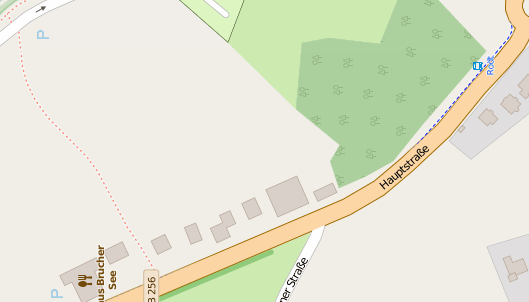
\includegraphics[width=\ScaleIfNeeded]{../chapter2/stuelinghausen@2-z17}
	\caption
		[straßenbegleitender Radweg von Straße verdeckt]
		{straßenbegleitender Radweg (blau strichliert) von Straße verdeckt \citex[rotiert]{map:osm-carto}}
	\label{fig:stuelinghausen-mapnik}
}

Abbildungen~\ref{fig:stuelinghausen-maps.me} und~\ref{fig:stuelinghausen-mapnik} zeigen beispielhaft, wie ein straßenbegleitender Radweg mal „über“, mal „unter“ der Straße zu liegen kommt.
Keiner dieser beiden Ansätze ist kartographisch gelungen.
Bevor eine Generalisierung durch Verdrängung stattfinden kann, muss zunächst der Konflikt zwischen Straße und Radweg erkannt werden.
Es ist denkbar, dass dies durch Untersuchen auf Parallelität geschehen oder erleichtert werden könnte.



\subsection{Generalisierung durch Zusammenfassung}

Die Generalisierung durch Zusammenfassung von Linienzügen kommt vor allem bei Parallelität in Betracht.
Dabei treten immer wieder in verschiedenen Situationen Darstellungsprobleme auf.

\label{dual-highway-case-2}

Beispielsweise variiert in OpenStreetMap auffallend oft der Abstand von zwei Richtungsfahrbahnen einer Straße.
Abbildung~\ref{fig:b256} zeigt, wie innerhalb weniger hundert Meter die Linearsignaturen zweier Richtungsfahrbahnen teilweise so weit voneinander entfernt liegen, dass dazwischen eine Lücke entsteht (Markierung~\textfiguremark{1}), aber teilweise auch so dicht beieinander, dass die Lücke geschlossen wird und die Randstriche der beiden Signaturen ineinander übergehen, was den Eindruck eines Mittelstriches wechselnder Strichstärke bewirkt (\textfiguremark{2}).
An einer Stelle sind die beiden Richtungsfahrbahnen gar so dicht beieinander gezeichnet, dass der Rand- bzw. Mittelstrich verschwindet und beide Fahrbahnen ineinander übergehen (\textfiguremark{3}).

\twofigures{ht}{
	\begin{overpic}[width=7cm]{../chapter2/b256@2-z16}
		\put(33,96){\figuremark[white]{1}}
		\put(96,81){\figuremark[white]{2}}
		\put(134,94){\figuremark[white]{3}}
	\end{overpic}
	\caption
		[variierende Abstände von Richtungsfahrbahnen]
		{variierende Abstände von Richtungsfahrbahnen \citex[bearbeitet]{map:osm-carto}}
	\label{fig:b256}
}{
	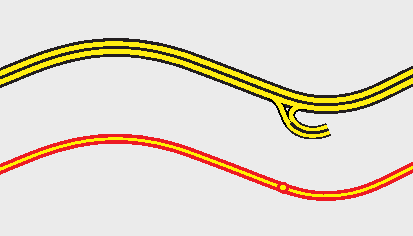
\includegraphics[width=\ScaleIfNeeded]{../chapter2/combined-symbols}
	\caption{kombinierte Signaturen für autobahnähnliche Straßen mit Anschlussstelle}
	\label{fig:dual-carriageway}
}

In Maßstabsbereichen, in denen die Grundrisstreue keine Rolle spielt, könnte möglicherweise eine stattdessen entlang der mittig zwischen den beiden Fahrbahnen verlaufenden Straßenachse gezeichnete kombinierte Signatur ein besseres Kartenbild erreichen (Abbildung~\ref{fig:dual-carriageway}).
Da jedoch in \osm\ die gesonderte Erfassung der Straßenachse unüblich ist, müssten hierzu zunächst die beiden Richtungsfahrbahnen als zusammengehörig (parallel) erkannt werden.

% TODO: evtl. Verweis auf ch2.1 / Sch09?
% siehe "Überleitung" unten!

% Grund für folgenden Absatz: zeigen, dass Verfahren von osm.de keine Lösung ist

In Deutschland erfasst die \osm-Community autobahnähnliche Straßen als \osmtag{highway}[trunk] anhand ihres Ausbauzustands.
Allerdings bildet die \osm-Straßenklassifizierung historisch bedingt das britische System ab, wo \term{trunk roads} ausdrücklich keinen bestimmten Ausbauzustand haben, sondern das Kernnetz der wichtigsten Straßen erster Ordnung bilden.
Unter Umständen wird \osmtag{highway}[trunk] somit auch für schmalere Landstraßen verwendet.

Wird den Gepflogenheiten in Deutschland entsprechend für \osmtag{highway}[trunk] eine auf den Ausbau mit baulich getrennten Fahrbahnen hindeutende Signatur gewählt, so birgt dies im internationalen Einsatz Potenzial für Verwirrung.
Abbildung~\ref{fig:trunk-norway-osm-de} zeigt eine solche Situation aus Norwegen:
Die Kartensignatur erweckt den Eindruck eines autobahnähnlichen Ausbaus, tatsächlich handelt es sich jedoch um eine einfache Landstraße mit Grundstückszufahrten und engen Kurvenradien (Abbildung~\ref{fig:trunk-norway}).

% TODO: Relationen-Probleme erläutern? -> eher weiter vorne!

% alternative Beispiele für schmale trunks in NO:
% Ev39 Kalandseidet, > 6 m aber Karte zeigt "mitten im Dorf"
% Ev39 Søfteland, Bild noch besser, aber keine Häuser in Karte
% Ev39 nach Nesttun rein, ginge auch, aber mit Radweg
%   https://goo.gl/maps/jYRgZVXft912
% Ev39 Vallaheiene wohl das beste hier
%   https://goo.gl/maps/wMHPCocqsSH2
% Rv13 Låtefossen, würde auch ohne Häuser in Karte funktionieren, < 6 m
% oder so Serpentinen, z. B. Granvin, gutes Bild aber keine Bebauung in Karte
%   https://goo.gl/maps/Y4NwWfRWSZ82

\twofigures{ht}{
	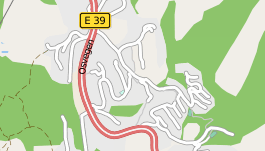
\includegraphics[width=\ScaleIfNeeded]{../chapter2/trunk-no-ev39-map1}
	\caption
		[Landstraße als {\osmtag{highway}[trunk]} mit autobahnähnlicher Signatur]
		{Landstraße (Vallaheiane) als {\osmtag{highway}[trunk]} mit \mbox{autobahnähnlicher} Signatur \citex{map:osm-de}}
	\label{fig:trunk-norway-osm-de}
}{
	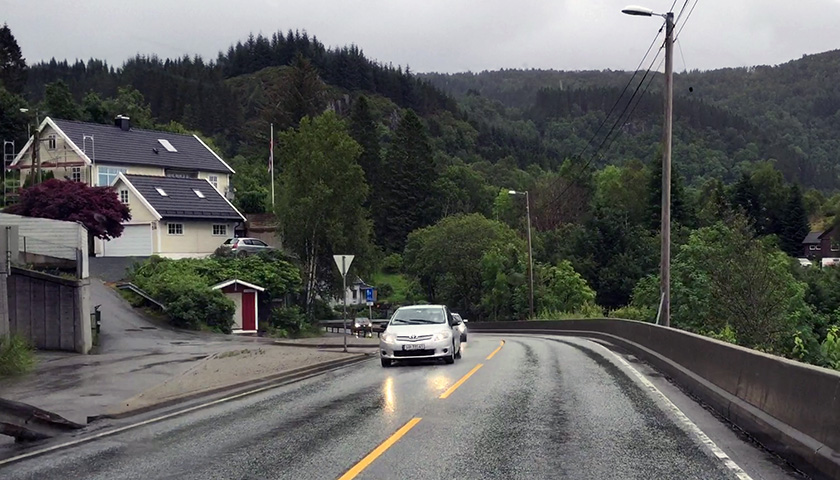
\includegraphics[width=\ScaleIfNeeded]{../chapter2/trunk-no-ev39-frame1639}
	\caption
		[typische norwegische Fernstraße \term{(riksveg),} als {\osmtag{highway}[trunk]} erfasst]
		{typische norwegische Fern\-straße (\term{riksveg} E\,39, Vallaheiane), als {\osmtag{highway}[trunk]} erfasst}
	\label{fig:trunk-norway}
}

Dass aus dem \osm-Datenmodell samt Attributen der tatsächliche Ausbauzustand oft nicht unmittelbar hervorgeht, macht die Möglichkeit einer algorithmischen Ableitung desselben aus der Geometrie der Geodaten interessant.
Möchte man einheitliche Zeichenregeln verwenden, so wäre auch hier die Möglichkeit einer Erkennung von zwei Richtungsfahrbahnen als parallel und zusammengehörig hilfreich.


% --------------------

% zu tracks=* - Überleitung evtl:
% Folge der oben beschriebenen offenen Arbeitsweise von \osm ist, dass das Herstellen einer Einigung über bestimmte Tagging-Varianten und deren Anwendung durch die Community oft ein langsamer Prozess ist. \noref[Sch09, forum 485926 s.u.]
% https://forum.openstreetmap.org/viewtopic.php?pid=485926

\label{railway-case}

Die Probleme durch fehlende Generalisierung durch Zusammenfassung sind nicht auf das Straßennetz beschränkt.
So wird in \osm\ mit \osmtag{tracks}[*] die Anzahl der Eisenbahngleise gekennzeichnet, für die ein \term{way} steht.
Die Karten in Abbildung~\ref{fig:tracks} stellen diesen \term{tag} farblich dar.

Bei Betrachtung in kleinem Maßstab sieht darin \textfiguremark{1} zunächst nach einer viergleisigen Strecke aus, in großem Maßstab plötzlich nach wenigstens \emph{zwei} viergleisigen Strecken nebeneinander.
Tatsächlich liegen insgesamt vier einzelne Gleise, die jeweils durch einen \term{way} mit dem Attribut \osmtag{tracks}[4] erfasst sind.%
\footnote{Die \osmtag{tracks}-Attribute wurden zwischenzeitlich durch Beitragende von diesen \term{ways} entfernt.}
In kleinem Maßstab fließen sie zusammen, in großem Maßstab sind sie jedoch einzeln erkennbar und vermitteln dem Leser das falsche Bild von insgesamt 16~Gleisen.
Möglicherweise hat ein \osm-Beitragender \osmtag{tracks}[*] missverstanden als die Gesamtanzahl der Gleise, \cf{Fox12} wofür jedoch das Attribut \osmtag{passenger\_lines}[*] zu verwenden ist.

% unklar, ob das Beispiel typisch war oder nicht
% (ich meine mich zu erinnern, dass der Fehler in GB stark verbreitet war, in DE eher untypisch)

\onedoublefigure{ht}{
	\begin{overpic}[width=\ScaleIfNeeded]{../chapter2/tracks-small}
		\put(92,63){\figuremark[white]{1}}
		\put(103,72){\figuremark[white]{2}}
		\put(95,13){\figuremark[white]{3}}
		\put(122,14){\figuremark[white]{4}}
	\end{overpic}
}{
	\begin{overpic}[width=\ScaleIfNeeded]{../chapter2/tracks-large}
		\put(33,75){\figuremark[white]{1}}
		\put(114,93){\figuremark[white]{2}}
		\put(76,10){\figuremark[white]{3}}
		\put(116,10){\figuremark[white]{4}}
	\end{overpic}
}{
	% fiktives Beispiel
	\caption
		[fehlerhafte Repräsentation der Gesamtzahl paralleler Gleise mit dem \osmtag{tracks}-Attribut]
		{fehlerhafte Repräsentation der Gesamtzahl paralleler Gleise mit dem \osmtag{tracks}-Attribut (links Zoom~15, rechts Zoom~17; Karlsruhe-Weiherfeld) \cf{map:ito-tracks}}
	\label{fig:tracks}
}

Analog kann in kleinem Maßstab der Eindruck entstehen, dass von der eingleisigen Strecke \textfiguremark{2} zwei doppelgleisige Strecken \textfiguremark{3} und \textfiguremark{4} derart abzweigen, dass am unteren Kartenrand insgesamt fünf Gleise nebeneinander liegen.
In größerem Maßstab wird erkennbar, dass es sich gerade umgekehrt verhält:
Die Strecke \textfiguremark{2} ist korrekt mit zwei parallelen Gleisen erfasst, deren Signaturen jedoch im kleineren Maßstab zusammenfließen;
die Abzweige \textfiguremark{3} und \textfiguremark{4} bestehen allerdings aus jeweils nur einem einzelnen Gleis, das fälschlich das Attribut \osmtag{tracks}[2] trägt.

% Fußnote?
Insgesamt sind die Darstellungen von \osmtag{tracks}[*] in Abbildung~\ref{fig:tracks} wenig gelungen.%
\footnote{Hier zeigt sich eine Schwäche von \osm: Zwar ist mit \term{relations} eine logische Verknüpfung paralleler Gleise in der \osm-Datenbank technisch möglich, jedoch ist dies nicht zuverlässig und simpel genug, dass es von einer Mehrheit der \osm-Beitragenden angewandt wird.}
Das unglücklich benannte Attribut \osmtag{passenger\_lines} reicht dazu aus, \osmtag{tracks}[*] für manche Anwendungen zu ersetzen, wird jedoch nur auf speziellen Karten angezeigt,
so dass es nicht annähernd flächendeckend erfasst ist (Abbildung~\ref{fig:passenger_lines}).%
\footnote{Bis Fertigstellung der vorliegenden Arbeit haben \osm-Beitragende das Attribut \osmtag{passenger\_lines} für die meisten europäischen Strecken ergänzt.}

\onefigure{ht}{
	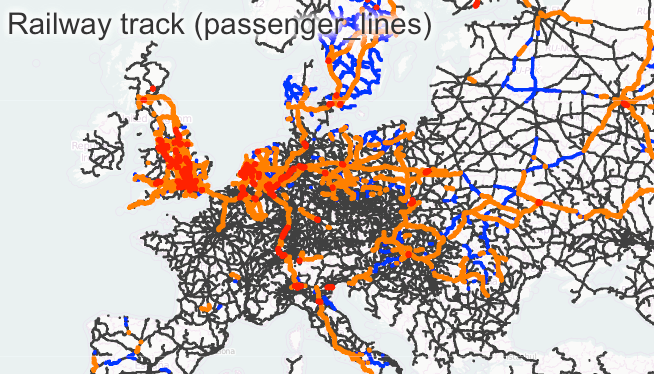
\includegraphics[width=\ScaleIfNeeded]{../chapter2/passenger_lines-europe}
	\caption
		[Eisenbahnstrecken in Europa, für die {\osmtag{passenger\_lines}[*]} erfasst ist]
		{Eisenbahnstrecken in Europa, für die \osmtag{passenger\_lines}[*] erfasst ist \citex{map:ito-passenger-lines}}
	\label{fig:passenger_lines}
}



%\subsection{Generalisierung durch Qualitätsumschlag}

%Beispiele für Qualitätsumschläge in Web-Karten sind schwierig zu finden. Oft handelt es sich bei entsprechenden graphischen Effekten technisch um eine Generalisierung durch Auswahl, durch die ein bisher verdecktes Element zum Vorschein kommt.



\section{Zielsetzung der Arbeit}

Das automatisierte Zusammenfassen paralleler Linienzüge kann zur Vermeidung einiger der oben diskutierten Probleme bei der Generalisierung und Darstellung von Geodaten beitragen.

Bereits das Zusammenfassen selbst ist ein Vorgang der kartographischen Generalisierung.
Es kann das Kartenbild vereinfachen und verbessern.

Beim Zusammenfassen könnten Attribute der beteiligten \term{ways} derart aggregiert werden, dass zuvor durch Geometrie ausgedrückte Zusammenhänge in den generalisierten Daten erhalten bleiben.
Beispielsweise könnte beim Zusammenfassen paralleler Gleise die in \osmtag{passenger\_lines} vermerkte Gleisanzahl der zuvor getrennten \term{ways} für das generalisierte Ergebnis addiert werden (vgl. Abschnitt~\ref{railway-case}).
Die so vereinfachten Geodaten können dann entsprechend ihrer Attribute visualisiert werden.
Die Gefahr von missverständlichen oder unschönen Kartenbildern, die wie oben gezeigt etwa durch Überlagerung entstehen können, wird so verringert.

Ebenfalls verringert wird die Datenmenge an sich.
Das Arbeiten mit Geodaten für große Gebiete, aber auch die Weiternutzung für andere Zwecke wird so unter Umständen einfacher.

Zum Beispiel sind automatisierte Formvereinfachungen einfacher durchzuführen, wenn keine Rücksicht auf eventuell parallele Linienzüge mehr genommen werden muss (siehe Abbildung~\ref{fig:crossing-parallels}).

% Zusammenfassung kann theoretisch auch Erstellen von MRDBs vereinfachen

Ziel \emph{dieser} Arbeit ist die Entwicklung von Algorithmen zur Generalisierung durch Zusammenfassung parallel verlaufender Linienzüge in \osm.
Weitere Generalisierungsvorgänge sind nicht Teil dieser Arbeit, insbesondere weder eine Formvereinfachung noch eine Verdrängung.



\section[Diskussion existierender Ansätze]{Diskussion existierender Ansätze zur automatisierten Linien-Generalisierung}
\label{ch:existing-approaches}

\subsection{Zusammenfassen durch Pufferung}
\label{ch:buffer}
% - für eine Darstellung von OSM-Daten als Teil eines 3D-Modells werden Straßen "realistisch" verbreitert per Buffer in PostGIS
% - um Fragmente und Parallelen zu beseitigen, werden die so entstandenen Polygone nun vereinigt
% => Parallelen finden durch Buffer-Algorithmus und Polygonanalyse
% => Epsilon benötigt
% - Buffer orthogonal zur Linie würde reichen; die Endrundungen können wegfallen
% - löst Zusammenfassung nicht, da keine unmittelbare Rückführung zur Linie allein mit diesem Ansatz möglich (was für das erklärte Ziel 3D aber eh nix ausmacht, insofern ist der Ansatz gut, aber eben nicht gut für mich); evtl. inward offset (um wieviel?) oder eher -> Skeleton
% - löst auch Erkennung nicht

Das Projekt „OSM-3D“ verwendet \osm-Daten automatisiert zum Aufbau eines 3D-Modells für die ganze Welt.
Die \term{ways} aus \osm\ werden für die 3D-Szene durch Pufferung mit attributabhängigem Radius in Polygone gewandelt, um ein Gesamtbild mit realistischen Breiten von Straßen, Wegen und Bahnlinien zu erzeugen.
Um dabei durch Überlappungen von eng parallelen \term{ways} entstehende unnötig große Datenmengen zu vermeiden, werden diese Polygone anschließend vereinigt. \cf[2–3]{OHSZ10}

Durch diesen Ansatz werden unerwünschte Parallelen beseitigt.
Allerdings ist die für diese Arbeit erwünschte Rückführung der durch die Pufferung entstandenden Flächen zu einer Linie nicht ohne Weiteres möglich.
Auch werden Parallelen nicht als solche erkannt, sondern entfallen restlos durch die Polygonvereinigung.
Daher erscheint dieser Ansatz isoliert betrachtet für die dieser Arbeit zugrundeliegende Fragestellung nicht geeignet.


\subsection{Bildung von Skelettlinien}
\label{ch:skeleton}
% - "In geometry, a straight skeleton is a method of representing a polygon by a topological skeleton." (<- Wikipedia)

Eine Möglichkeit, Flächen auf innere Linien zu reduzieren, bietet die Skelettierung.
Für das \term{straight skeleton} werden Polygone so lange sukzessive geometrisch verkleinert, bis nur noch ein aus geraden Linien zusammengesetztes topologisches Skelett übrig bleibt (Abbildung~\ref{fig:skeleton}).
Hierfür existieren unterschiedliche Algorithmen. \cf{wp:StraightSkeleton}

\onefigure{bt}{
	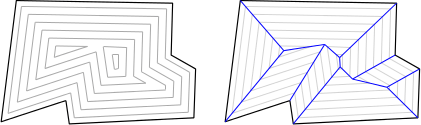
\includegraphics[width=9cm]{../chapter2/approach-skeleton}
	\caption
		[sukzessive Verkleinerung einer Fläche und deren Skelettlinien]
		{sukzessive Verkleinerung einer Fläche (links) und deren Skelettlinien (blau; rechts) \citex{Hub12}}
	\label{fig:skeleton}
}

% HS04: straight skeleton for MRDB
% <http://web.archive.org/web/20070613154012/http://www.ikg.uni-hannover.de/skalen/buendel/PDF/Skeleton.pdf>
% - Ziel: Framework für MRDB (automatisch)
% - erwähnt Chordal Axis (Prasad, 1997) ********
% - verwendet straight skeleton plus eine handvoll Regeln, um Kreuzungen etc. zu behandeln; immer noch etwas verwurstet, aber sieht wesentlich besser/systematischer aus als LM96
% - schlägt angeblich fehl an komplizierteren Stellen
% - ermittelt eine Relation zwischen ALK ATKIS

\Citeauthor{HS04} nutzen ein \term{straight skeleton}, um aus Flächen in der Automatisierten Liegenschaftskarte (ALK) Linien zur Nutzung in einer Multiple Representation Database (MRDB) abzuleiten.
Der Algorithmus von \citeauthor{EE99} \citex{EE99} musste für die ALK-Daten angepasst und erweitert werden, um das resultierende Straßennetz auf die gewünschten Mittellinien der Flächen zu reduzieren.
Dennoch kommt es zu teils erheblichen Problemen an Kreuzungen, die nicht in allen Fällen gelöst werden können. \cf[4–6]{HS04}

% Mig12: Projekt für "schöne" topo. Karte
% <http://mike.teczno.com/notes/osm-us-terrain-layer/foreground.html>
% <http://mike.teczno.com/img/terrain-stamen-post/> *******
% - erwähnt kurz Probleme von dual carriageways
% - eines der Probleme: unschöne versetzte Doppelungen von Straßennamen
% - Anwendung von Skeletron (mit Implementierung von LM96 für OSM)
% - Ziel letztlich "nur" Shields und Straßennamen

\Citeauthor{Mig12} setzt eine Skelettierung ein, um für eine topographische Karte auf \osm-Basis Straßennamen und -nummern graphisch ansprechend darzustellen.
Im Falle von zwei zueinander parallelen Fahrbahnen derselben Straße sollen Nummer und Name so gezeichnet werden, dass sie für beide Fahrbahnen gelten und unschöne Doppelungen des Namens vermieden werden.
Hierzu benutzt Migurski die Software Skeletron. \citetext{\citealp{ME11}, cf. \citealp{Mig12}}

% Skeletron [ME11]:
% <https://github.com/migurski/Skeletron>
% - jetzt LM96, davor HS04 (?) "straight skeleton", was nicht so toll war

Skeletron benutzte ursprünglich ein \term{straight skeleton} nach dem erwähnten Ansatz von \citeauthor{HS04}, was aber letztlich nicht besonders gut funktioniert hat („ultimately didn't work very well“ \citex[Readme]{ME11}).
Inzwischen wird die von \citeauthor{LM96} für diesen Zweck beschriebene Thiessen-Polygon-Methode eingesetzt.

% LM96: Straßen_flächen_ -> Einzellinie
% - Ziel: Eliminierung _oder_ Minimierung manueller Eingriffe
% - gute Ausgangsdaten seien entscheidend fürs Projekt gewesen (1:1000, mit Straßenflächen!)
% - ways werden verdichtet auf einen node alle 30 cm, um eine gesmoothte Mittellinie zu erhalten
% - ausgehend von nodes wird ein Voronoi-Diagramm gebaut, aus dem sich direkt die Mittellinie ergibt (nach filtern)
% - erzeugt schwierig zu filternde Dangles / Forks dort, wo Parallelen enden; Auflösung durch zusätzliche Angaben aus der Datenquelle ('The "true end" of the road is determined by temporarily appending the appropriate road extent arcs from the original Urban layer.')
% - "Suspect situations" kommen vor und werden manuell beseitigt
% - 7 man-months

Hierbei werden ausgehend von einer sehr detaillierten Straßenfläche zunächst deren Kanten verdichtet auf mehrere Knoten pro Meter, bevor ausgehend von diesen Knoten mittels Delaunay-Triangulierung ein Voronoi-Diagramm berechnet wird, dessen Kanten die Skelettlinien der Straßenfläche sind.
Auch hier ergeben sich allerdings erhebliche Probleme an allen Kreuzungen, die trotz Einbeziehung von Metadaten nur teilweise automatisch gefiltert werden.
Solche Fälle können immerhin automatisch erkannt und dann manuell beseitigt werden.
Der Aufwand für die Implementierung wird mit sieben Personenmonaten beschrieben. \cf{LM96}

Um aus den \osm-\term{ways} Flächen zu erhalten, mit denen das Anwenden der Thiessen-Polygon-Methode erst möglich wird, puffert Skeletron zuvor die \osm-\term{ways} wie in Abschnitt~\ref{ch:buffer} beschrieben. \cf{ME11}


\subsection{Konflikterkennung}
\label{ch:conflict-detection}

%\item Conflict Detection \cf{KP98} \cf{Tho06a}
% KP98:
% - Ziel: gesamtes Straßennetz
% - detektiert Fälle, in denen Linien einander zu nahe kommen (wobei Bereiche nahe der Endknoten jeweils ausgeschlossen werden)
% - nutzt Voronoi region
% - eigentlich nicht speziell für parallelen gedacht oder geeignet (nutzt Dijkstra, um längeren von zwei Wegen zu eliminieren), aber speziell der "Second step: eliminate conflicts" könnte anwendbar sein, und der Voronoi-Kram gibt zumindest ein paar hübsche Bilder

\Citeauthor{KP98} beschreiben eine Möglichkeit, bei der automatischen Ableitung von Straßenkarten Konflikte nahe beieinander liegender Straßen zu erkennen und durch Auswahl nur einer der beteiligten Straßen aufzulösen.
Neben anderen Bedingungen werden so auch graphische Mindestabstände eingehalten. \cf{KP98}

Es liegt auf der Hand, dass sich parallele Straßen meist durch ein Unterschreiten dieser Mindestabstände auf ihrer gesamten Länge auszeichnen.
Das beschriebene Verfahren untersucht allerdings lediglich den minimalen Abstand zweier Straßen.
Das Untersuchen der gesamten Länge der Straße wäre erheblich teurer. \cf[4.]{KP98}
Dieser Ansatz erscheint daher für diese Arbeit wenig erfolgversprechend.

% Tho06a: ? Bib, einzelne Fotos in "neu"
% - erwähnt ausdrücklich mein Problem als "hilfreich" (in gelöstem Zustand)
% - Skeleton??

\Citeauthor{Tho06a} erwähnt ausdrücklich, dass die Erkennung eines Konflikts von parallelen Straßenabschnitten für die automatische Generalisierung hilfreich wäre („... recognizing stretches of parallel road sections would help their automatic generalization“ \citex[676]{Tho06a}), allerdings ohne dabei eine mögliche Lösung anzudeuten.


%\subsection{Kognitive Wahrnehmung}
\subsection{Visuelle Wahrnehmung}

% Tho06b: Netzwerk-Generalisierung und -Analyse
% - perzeptueller Ansatz zur Defragmentierung und Auswahl-Generalisierung
% - primär Behandlung kollinearer Linien, erwähnt beiläufig aber auch Erkennung von Parallelen [evtl. mehr in den zahlreichen Referenzen darin?]
% - "perceptual grouping" [684]

\Citeauthor{Tho06b} beschreibt, wie das menschliche Gehirn optisch wahrgenommene Elemente selbst dann „spontan organisiert“, wenn deren Semantik völlig unbekannt ist.
Er bezeichnet dieses Konzept als „perceptual grouping“ und zählt unter den dazu herangezogenen geometrischen Eigenschaften neben Nähe, Ähnlichkeit und Symmetrie auch Parallelität und Kontinuität auf. \cf[683–684]{Tho06b}

% EM00:
% - erwähnt sehr deutlich meine Probleme mit "hanging streets" an Kreuzungen etc. [3]
% - erwähnt keine Parallelen, zeigt aber Implementierung der Theorien von Tho06b bzw. TR99

Zusammen mit Richardson beschreibt er eine Möglichkeit, die Eigenschaft der Kontinuität von Linienzügen (genannt \term{stroke}) zu nutzen, um deren Wichtigkeit einzustufen und damit ein Straßennetz zu generalisieren („Principle of Good Continuation“, Abbildung~\ref{fig:strokes}). \cf{TR99}
\Citeauthor{EM00a} nutzen denselben Ansatz zur Analyse des Netzes, um damit ihre auf Graphentheorie basierende Generalisierung zu unterstützen. \cf{EM00a}
Wie ein „perceptual grouping“ nach der Eigenschaft der Parallelität aussehen könnte, wurde nach Kenntnis des Verfassers bisher nicht konkret untersucht.

\onefigure{hb}{
	\includegraphicsmaybe{../chapter2/approach-strokes_51}
	% copyrighted image used under § 51 UrhG - not included in git repository
	\caption
		[ein Netzwerk und seine \term{strokes} {[\copyright]}]
		{ein Netzwerk (a) und seine \term{strokes} (b) \citex[\term{figure} 2][\copyright]{TR99}}
	\label{fig:strokes}
}

% ! OS MasterMap
% CM05: ganzheitlicher Ansatz für Ordnance Survey in Road Network
% - arbeitet primär mit Strokes; Problem dabei: "good continuation" sieht an Gabelungen u. U. je nach Seite unterschiedlich aus; zur Lösung werden Attribute herangezogen
% - Fig 10 zeigt Resultat, welches Parallelen hat, welche nicht erwähnt werden
% - hebt Kreuzungsproblem als ungelöst hervor

\Citeauthor{CM05} schlagen das Konzept von \term{strokes} zur Generalisierung von Straßennetzen durch Auswahl wichtiger Straßen für die digitale OS~MasterMap des Ordnance Survey vor.
Sie betonen jedoch, dass trotz ermutigender Resultate noch weitere Probleme gelöst werden müssen.
Auf die Eigenschaft der Parallelität gehen sie nicht ein. \cf{CM05}

% (ähnelt grob meinem Ansatz)
% Tho05: speziell meine Problemstellung!
% - Ziel: Hilfe bei automatischer Folgekartenableitung beim Ordnance Survey
% - 3 wichtigste Teile: Kreuzungsproblem, Verdrängung und Zusammenfassung von Parallelen [2]
% - arbeitet mit Strokes basierend auf one-way-Attributen; Probleme an manchen Kreuzungen, die aber automatisch erkannt und behoben werden sollen
% - Paarbildung erfolgt abhängig von Klassifizierung der Strokes (z. B. bei Verkehrsinseln kleinere Höchstschwelle als bei normalen Straßen)
% - Ausgangsdaten sind klassifiziert nach "dual carriageway" oder nicht (DESHALB nicht 1:1 auf OSM anwendbar, denn es gibt keinen solchen tag)
% - klappt nicht in allen Fällen (einzelne Fehlerfälle)
% - benutzt Skeleton zur tatsächlichen Zusammenfassung der erkannten Paare
% - funktioniert meistens, aber nicht immer; manche der Restfälle manuell als nicht lösbar erkannt
% - one-way-Attribut war "essential"
% - Ergebnis hat noch keine Topologie (future work)
% - erst mit Topologie ist Unterbrechung der Signatur möglich, um Ampelkreuzungen im Dual Carriageway darzustellen
% - Kreisverkehre werden bisher ignoriert

\label{os-mastermap}

\Citeauthor{Tho05} beschreibt vier Schritte zum Zusammenfassen getrennter Richtungsfahrbahnen von zweibahnigen Straßen und Verkehrsinseln auf eine gemeinsame Mittellinie für die OS~MasterMap.
Zunächst werden unter Nutzung von \term{strokes} und Attributen durchgehende Linienzüge für die Gesamtlänge der getrennten Richtungsfahrbahnen erzeugt, die dann durch Graphenanalyse ihrer jeweiligen Enden einander zugeordnet werden können.
Anschließend kann durch Skelettierung die Mittellinie der zugeordneten Linienzüge berechnet und im letzten Schritt noch Korrekturen an deren Enden vorgenommen werden. \cf[3–10]{Tho05}

Diese Schritte liefern in vielen Fällen ein gutes Ergebnis, was \citeauthor{Tho05} der Attribuierung der Ausgangsdaten zuschreibt.
Entscheidend ist insbesondere das „one~way“–Attribut sowie die Klassifikation nach Bauart der Straße (einbahnig, zweibahnig, Verkehrsinsel, Kreisverkehr etc.). \cf[14]{Tho05}


\subsection{Graphenanalyse}
\label{ch:graph-based}

% TR95: Graphentheorie in der Generalisierung von Straßennetzen
% - betont, dass autom. Generalisierung oft Darstellungs-zentriert ist und Topologie des Ergebnisses vernachlässigt [1871]

% MB93: Graphentheorie in der Generalisierung allgemein
% - durch Prüfung der Einbahn-Richtung erkennen, ob insgesamt ein verbundener Graph vorliegt (zweimal Einbahn => einmal Zweibahn)

Frühe Entwicklungen der automatisierten Generalisierung versuchten oft, unter Vernachlässigung der Topologie des Ergebnisses den Fokus des Kartographen auf der Visualisierung nachzuahmen. \cf[1871]{TR95}
Ansätze der Graphentheorie können jedoch nicht nur wie zuvor beschrieben andere Methoden unterstützen, sondern auch direkt zur Generalisierung eingesetzt werden.

% HAS05: will typische Muster erkennen
% - erwähnt für Strokes Problem dort, wo Richtungsfahrbahnen beginnen, mitsamt theoretischer Lösung [3.2]
% - evtl. können Parallelen in einem Netzwerk durch Musteranalyse erkannt werden (typischerweise sehr lang und schmal); jedoch vmtl. Probleme an Kreuzungen etc.

\Citeauthor{HAS05} zeigen Methoden, um typische Muster in Straßennetzen zu erkennen und daraus Informationen abzuleiten. 
Es liegt auf der Hand, dass parallele Fahrbahnen einer zweibahnigen Straße ein typisches Muster sein können, jedoch werden diese nur beiläufig erwähnt. \cf[3.2.]{HAS05}

% JC04: connectivity graph für urban street network
% - dreht Straßen-Graph logisch um (Knoten=Straße, Kante=Verbindung)
% - filtert nach Graphkriterien ("centralities" degree, closeness, betweenness)
% - Ergebnis ist ein nach natürlich Kriterien modellgeneralisiertes Netz, denn Straßen mit besserer Verbindung werden häufiger benutzt und sind somit wichtiger
% - Parallelen im Straßennetz zeichnen sich durch Redundanz und Symmetrie aus (oft gegeneinander gerichtete Einbahnstraßen) und sind damit höchstens! in einem sehr unregelmäßigen Netz theoretisch! erkennbar; tatsächlich werden im Beispiel im Paper die Parallelen nicht generalisiert [168]

\Citeauthor{JC04} verwenden Zentralitätsmaße, um die wesentliche Struktur eines Straßennetzes zu identifizeren und bei der Generalisierung zu erhalten.
Dieser Ansatz entspricht dem Prinzip, dass schlechter ans Netz angebundene Straßen weniger wichtig sind als jene, die gut angebunden sind („less connected streets are less important than those well connected from a structural point of view“ \citex[161]{JC04}). \cf{JC04}
Für parallele Kanten im Graph ist allerdings zu erwarten, dass sie jeweils ähnlich gut an den Rest des Netzes angebunden sind, weswegen dieses Kriterium für diese Arbeit nicht als nützlich erscheint.

% MM99: Simplification of Junctions
% - "Brücken von Königsberg" als Beispiel für junction simplification und Zusammenfassung von Parallelen, aber das ist wohl etwas zu sehr vereinfacht! [188]
% - evtl. werden durch Zusammenfassen der Kreuzung von Parallelen jene zu Duplikaten und können so erkannt und zusammengefasst werden; Nachteil: klappt wirklich nicht ohne Kreuzungen (diese Methode wird anscheinend nicht explizit erwähnt)

Probleme an Kreuzungen wurden bereits von mehreren Autoren genannt.
\Citeauthor{MM99} demonstrieren eine Methode, um Straßenkreuzungen durch eine Kombination von räumlicher und graphentheoretischer Analyse zu identifizieren und zu vereinfachen. \cf{MM99}

Der Gedanke, dass etwa im Falle einer zweibahnigen innerstädtischen Straße durch Generalisierung komplexer Kreuzungen auf einen einzelnen Punkt die vormals nur geometrisch parallelen Kanten zu zwei topologisch parallelen Kanten (Mehrfachkanten) in einem ungerichteten Graphen des Straßennetzes werden, welche dann leicht zusammenzufassen sind, liegt im Kontext dieser Arbeit nahe (Abbildung~\ref{fig:graph-edges-parallel} verdeutlicht dies anhand von als parallel geltenden Brücken).
Die Arbeit von \citeauthor{MM99} berücksichtigt diesen Aspekt allerdings nicht.

\onefigure{ht}{
	\includegraphicsmaybe[width=11.4cm]{../chapter2/graph-edges-parallel_51}
	% copyrighted image used under § 51 UrhG - not included in git repository
	\caption
		[graphentheoretische Form des „Königsberger Brückenproblems“ und eine Reduktion des Graphen {[\copyright]}]
		{das „Königsberger Brückenproblem“ (a), seine graphentheoretische Form (b) und eine Reduktion des Graphen (c) \citex[188][\copyright]{MM99}}
	\label{fig:graph-edges-parallel}
}



%\begin{itemize}
%\item \cf{Kne09}
% Kne09: Anwendung von Graphentheorie in OSM, wenig hilfreich für uns
% ! Relational Constraints
%\item Relational Constraints \cf{TBDJRG12}
% - hat keinen Algorithmus, sondern nur Konzepte
% - führt constraint ontology ein als mögl. Hilfswerkzeug
% evtl. als Grundlage für Kap. 4 interessant
%\end{itemize}

% + RoadMatcher 
% <http://wiki.openstreetmap.org/wiki/Roadmatcher>
% + http://sourceforge.net/projects/jump-pilot/files/OpenJUMP_plugins/More%20Plugins/Matching%20PlugIn/
% <http://sourceforge.net/projects/jump-pilot/files/OpenJUMP_plugins/More%20Plugins/Matching%20PlugIn/>



% single-chapter commands
\onlyinsubfile{\listoffigures} %\onlyinsubfile{\listoftables}
%\onlyinsubfile{\subfile{../bibliography/Literaturverzeichnis}}
\end{document}

% UTF-8

% single-chapter commands
\documentclass[../main/thesis.tex]{subfiles}
\onlyinsubfile{\setcounter{chapter}{2}}  % single-chapter command
\begin{document}


\chapter{Spezifikation der zu untersuchenden Fälle}

% Plural oder Singular?
% (vgl. Themenblatt)

% Probleme aus Kap. 2, die in 3 aufgegriffen werden könnten:
% - 2.3.3 Bewertung: Croeselaan
% - 2.3.4 Formvereinfachung: Überkreuzen


\section{Vergleich verschiedener Problemfälle der automatisierten Linien-Ge\-ne\-ra\-li\-sie\-rung}
\label{ch:case-comparison}

% (Vergleich unter dem Gesichtspunkt der Eignung als „Spezialfall“ für diese DA, vgl. Themenblatt)
% evtl. jeweils ein (Ab)satz zu "worum genau geht es bei diesem Problem" (was nur teilweise offensichtlich ist) und ein (Ab)satz zur Eignung

An dieser Stelle werden zunächst unterschiedliche Spezialfälle beschrieben, in denen die automatisierte Identifikation und Zusammenfassung parallel verlaufender Linienzüge hilfreich wäre.
Der darauf folgende Abschnitt begründet die Auswahl der entsprechend der Aufgabenstellung im Rahmen dieser Arbeit im Weiteren zu behandelnden Spezialfälle.


\subsection{Mehrgleisige Eisenbahnstrecken}

Das Problem der Auswertung der Gleisanzahl mehrgleisiger Bahnstrecken ist bereits in Abschnitt~\ref{railway-case} beschrieben.
Neben der Erkennung solcher Gleise als parallel kann die geometrische Ermittlung der Bahnachse hilfreich für eine ansprechende Visualisierung sein.
Lagepläne im Eisenbahnwesen zeigen sie zusätzlich zu den Gleisachsen, in \osm\ wird sie jedoch nicht erfasst.

% "Bahnachse" https://www-docs.tu-cottbus.de/verkehrswesen/public/Lehre/Lehrbuch/Grundlagen/0-3Zeichnung.pdf


\subsection{Richtungsfahrbahnen im Straßenraum mit baulicher Trennung}
\label{ch:dual-highway-case-desc}

Auch für zweibahnige Straßen, welche in \osm\ als zwei parallele Linienzüge modelliert sind, wird im Gegensatz zum deutschen amtlichen Vermessungswesen \cf[107]{adv08} in \osm\ keine Mittellinie als Achse der Straße erfasst.
Die sich daraus für \osm\ ergebenden Probleme wurden bereits in Abschnitten~\ref{dual-highway-case-1} und~\ref{dual-highway-case-2} beschrieben.
Konkrete Beispiele für solche Straßen sind Autobahnen, aber auch zweibahnige innerstädtische oder Überlandstraßen.

% ATKIS-Objektartenkatalog Basis-DLM 6 (2008)
% http://www.geodatenzentrum.de/docpdf/ATKIS-OK%20Basis-DLM%206_0.pdf


\subsection{Parallele Wege für unterschiedliche Arten von Verkehr}
\label{ch:different-traffic-types-case-desc}

Ein oft zu beobachtendes Muster sind zusammengehörende, jedoch baulich getrennte und damit jeweils als eigene Linienzüge modellierte Verkehrswege für unterschiedliche Fahrzeugtypen, Geschwindigkeitsbereiche oder Zwecke des Verkehrs.
Im Straßenraum zählen dazu:

\begin{itemize}
	\item straßenbegleitende Fuß- und Radwege,
	\item Nebenfahrbahnen \term{(frontage roads)} für Anliegerverkehr, von dem die Hauptfahrbahn freigehalten werden soll,
	% Beispiele: Autobahnen, Kaiserstraße
	\item langgezogene Rampen an teilplanfreien Anschlussstellen insbesondere der Bauformen Diamant und \term{SPUI,}
	% https://de.wikipedia.org/wiki/Anschlussstelle_(Autobahn)
	\item Verteilerfahrbahnen an Doppelanschlussstellen und Autobahnkreuzen,
	% https://de.wikipedia.org/wiki/Autobahnkreuz#Bauteile
	% https://de.wikipedia.org/wiki/Doppelanschlussstelle
	\item Sonderfahrbahnen für Busse, Fahrgemeinschaften oder Mautzahler,
	% https://de.wikipedia.org/wiki/High-occupancy_vehicle_lane#Ausf.C3.BChrung
	\item straßenbündige oder -parallele Bahnkörper,
	\item die Kombination mehrerer der genannten Punkte, etwa als Teil einer komplexen innerstädtischen Straße mit parallelen getrennten Radwegen, Gehwegen, Richtungsfahrbahnen, Nebenfahrbahnen und besonderem Stadtbahn-Gleiskörper.
\end{itemize}

Die sich in solchen Fällen ergebenden Probleme sind vergleichbar zu Abschnitt~\ref{ch:dual-highway-case-desc}, jedoch komplexer, weil die beteiligten Verkehrsarten jeweils unterschiedliche Voraussetzungen haben.
So sind z.~B. straßenbegleitende Radwege aufgrund der geringeren gefahrenen Geschwindigkeiten oft kurviger als die Fahrbahn für Kraftfahrzeuge, sollten aber dennoch als parallel zu ihr gelten können.
Auch erfordern die Unterschiede in Kombination mit Platzmangel oft individuelle bauliche Lösungen, was die Automatisierung der Verarbeitung der Geodaten nicht vereinfacht.


\subsection{Grenzen}

Bisher noch nicht erwähnt wurden unsichtbare Grenzen, deren Verlauf dem physischer Objekte folgt oder zu ihnen parallel ist.
Beispielhaft zu nennen wären Postleitzahlgebiete, deren Grenze einem Straßenzug folgt, oder administrative Grenzen entlang eines Wasserlaufs.
In diesen Fällen kann in der Kartographie die Grenze vom verlaufsgebenden Objekt abgesetzt werden, damit beide Signaturen klar erkennbar sind. \cf[82]{sgk02}
Auch eine Unterbrechung der Signatur ist möglich (Abbildung~\ref{fig:administrative-borders}).
In \osm-Karten ist eine solche Generalisierung bisher noch nicht üblich.
% wie werden die Daten statt dessen umgesetzt?
% Streit, ob Unsichtbares überhaupt in OSM rein soll

\begin{figure}[ht]
  \begin{minipage}[t]{.5\linewidth}
    \centering
    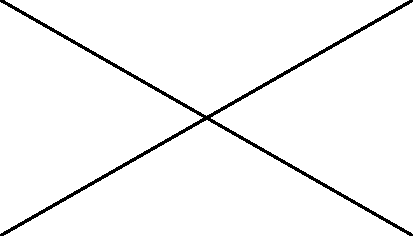
\includegraphics[width=\ScaleIfNeeded]{../image-missing}
    \caption{administrative-borders}\label{fig:administrative-borders}
  \end{minipage}%
  \begin{minipage}[t]{.5\linewidth}
    \centering
    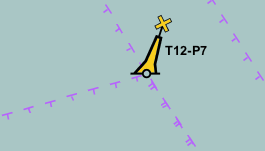
\includegraphics[width=\ScaleIfNeeded]{../chapter3/restricted-area-oseam}
    \caption{restricted-area-oseam}\label{fig:restricted-area-oseam}
  \end{minipage}
\end{figure}

Ein weiteres Beispiel sind zwei aneinander angrenzende Gebiete mit Schifffahrtsbeschränkungen.
Nach den Zeichenregeln für Seekarten ist in solchen Fällen die übliche T-Signatur \cf[B-439.2]{iho13} nur für das gefährlichere der beiden Gebiete zu zeichnen („For coincident limits, the limit symbol (line) portraying the area which is considered to be potentially the most dangerous to navigation [...] has priority.“ \citex[B-439.6~a.]{iho13}).
% S4_4.4.0_EN_Sep13
Eine derartige Abwägung dürfte zwar schon aus rechtlichen Gründen nicht automatisationsfähig sein.
Eine Verbesserung der gegenwärtig unbefriedigenden Darstellung in der auf \osm-Daten basierenden Karte „OpenSeaMap“ (Abbildung~\ref{fig:restricted-area-oseam}) wäre allerdings möglich und anzustreben.

Insgesamt erscheinen Grenzen jedoch im Kontext dieser Arbeit als ein eher schwieriges Feld.
%Während in bestimmten Fällen die üblichen \osm-Karten klare Defizite haben, sind die Fälle, in denen Parallelität eine Rolle spielt, unregelmäßig und 
% Geht das vielleicht schon zu weit?


\subsection{Grundrisstreu erfasste linienhafte Objekte}
\label{ground-plan-linear-objects-case-desc}

Mit zunehmendem Grad der Detaillierung in \osm\ wird versucht, eigentlich linienhafte Objekte als grundrisstreue Fläche zu erfassen.
Für Flüsse ist dies bereits üblich \cf[72]{RT09}, für Straßen und Rollbahnen unter Diskussion.
% http://wiki.openstreetmap.org/w/index.php?title=Key:area&oldid=865108#Highway.2Fpavement_areas
% http://wiki.openstreetmap.org/w/index.php?title=Tag:aeroway%3Drunway&oldid=1218356#How_to_Map
Dadurch entstehen sehr lange und schmale Flächen, deren Ränder größtenteils parallel zueinander sind.
Wenigstens bei Flüssen ist es allerdings etabliert, zusätzlich zur Fläche auch eine Mittellinie in \osm\ zu erfassen.
Daher stellen diese Fälle in der Praxis kein Problem dar und sind für diese Arbeit nicht weiter interessant.


\subsection{Vegetationsgrenzen entlang von Verkehrswegen}

Ein Sonderfall der in Abschnitt~\ref{ground-plan-linear-objects-case-desc} beschriebenen langen und schmalen Flächen sind Waldschneisen.
Im Zuge der immer detaillierteren Erfassung nicht nur des Wegenetzes, sondern auch der Vegetation kommt es vor, dass zusätzlich zu einem durch den Wald führenden Weg auch die sich durch den Weg ergebende Schneise im Wald erfasst wird, indem die Waldfläche in \osm\ in zwei Flächen links und rechts des Wegs aufgeteilt wird (Abbildung~\ref{fig:vegetation-swath-z16}).

Einerseits ermöglicht dies eine präzisere Modellierung der Wirklichkeit, indem die womöglich die Breite des Wegs übersteigende Breite der Schneise modelliert werden kann.
Andererseits werden große Wälder ohnehin gerne in mehrere kleinere Flächen aufgeteilt, um das Arbeiten mit den Geodaten zu vereinfachen.
Schneisen bieten sich dabei als natürliche Stelle zum Aufteilen an.

\begin{figure}[ht]
  \begin{minipage}[t]{.5\linewidth}
    \centering
    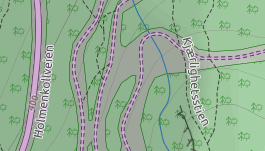
\includegraphics[width=\ScaleIfNeeded]{../chapter3/vegetation-swath-z16}
    \caption{Waldbegrenzung in dieser \osm-Karte dargestellt durch grüne Linie, \term{zoom}~16 (©~Thunderforest)}\label{fig:vegetation-swath-z16}
  \end{minipage}%
  \begin{minipage}[t]{.5\linewidth}
    \centering
    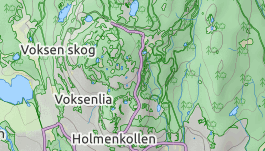
\includegraphics[width=\ScaleIfNeeded]{../chapter3/vegetation-swath-z12}
    \caption{in kleinerem Maßstab Waldschneisen durch grüne Linien unangemessen betont, \term{zoom}~12 (©~Thunderforest)}\label{fig:vegetation-swath-z12}
  \end{minipage}
\end{figure}
% http://www.thunderforest.com/maps/landscape/

Je nach den verwendeten Zeichenregeln werden solche Schneisen in \osm-Karten jedoch stärker betont als wünschenswert (Abbildung~\ref{fig:vegetation-swath-z12}).
Hier wäre eine Erkennung der parallelen Ränder der Schneise hilfreich, um durch Zusammenfassen der Waldfläche das Kartenbild zu verbessern und gleichzeitig zu verhindern, dass durch diese Art der Modellierung entstehende kleinere, von Schneisen umringte Waldparzellen aufgrund von Mindestgrößen automatisch wegfallen.

% allerdings vielleicht hier puffer-methode besser geeignet, schließlich geht es eigentlich um die fläche


%\subsection{Bachläufe und Verkehrswege}
%% das klassische Problem
%
%…





\section{Auswahl der in dieser Arbeit zu behandelnden Spezialfälle}

Viele der bisherigen Arbeiten zur automatisierten Zusammenfassung haben sich mit Straßen beschäftigt (Abschnitt~\ref{ch:existing-approaches}).
In mehreren dieser Arbeiten betonten die Autoren die Wichtigkeit von Ausgangsdaten mit hoher Qualität.
Im Falle von OpenStreetMap ist zu erwarten, dass die Datenqualität für Elemente des Straßennetzes höher ist als die von manch anderen Elementen der \osm-Datenbank.

So gibt es Anhaltspunkte für eine Korrelation zwischen Datenqualität und dem Umstand, ob diese Daten in der Standard-Visualisierung dargestellt werden. \cf[18]{NZZ11}
Dies ist auch anschaulich klar, denn leicht sichtbare Fehler fallen schneller auf und werden somit auch schneller korrigiert als andere Fehler.
Die Standard-Visualisierung der Karte auf \href{https://www.openstreetmap.org/}{\nolinkurl{osm.org}} berücksichtigt viele Details des Straßennetzes.
Unter anderem werden Name und Nummer von Straßen dargestellt, nicht jedoch beispielsweise von Eisenbahnstrecken.
% Highways: Tags für viele Details existieren und werden genutzt. Mehr als für Railways? Vergleich evtl. durch TagInfo möglich, entweder mit historischen Daten (Geofabrik?) oder aber mit aktuellen plus qualitative Überlegung (wann entstand openrailwaymap?)
% TODO: ist der logische Fluss hier ausreichend explizit?

Hinzu kommt die hohe praktische Relevanz des Straßennetzes, die bereits im Namen „OpenStreetMap“ Ausdruck findet, für die \osm-Beitragenden genau wie auch für die Allgemeinbevölkerung.
\osm-Daten werden nicht mehr nur zur visuellen Darstellung, sondern auch zur Navigation verwendet.
Auch dies geht mit einer erhöhten Datenqualität einher. \cf[17–18]{NZZ11}
% Quelle für diesen Punkt nicht großartig; kann dies anhand von Changesets quantifiziert werden?
Verbesserte Algorithmen könnten hier besonders vielen Nutzern zugutekommen.
% TODO: ist der logische Fluss hier ausreichend explizit?

Aus diesen Gründen wird von den zuvor in Abschnitt~\ref{ch:case-comparison} beschriebenen Anwendungsfällen für eine automatisierte Linienzusammenfassung der Fall von \textbf{baulich getrennten Richtungsfahrbahnen im Straßenraum} für diese Arbeit ausgewählt (Abschnitt~\ref{ch:dual-highway-case-desc}).
Solche Straßen sind nahezu allgegenwärtig und die mit deren Darstellung verbundenen Probleme verbreitet.

Die in Abschnitt~\ref{ch:different-traffic-types-case-desc} beschriebenen Fälle paralleler Wege für unterschiedliche Verkehrsarten bieten sich aufgrund ihrer Komplexität nicht an, solange nicht der einfachere Fall von Richtungsfahrbahnen zufriedenstellend gelöst ist.
Es ist jedoch denkbar, dass eine Lösung für bauliche getrennte Richtungsfahrbahnen auch auf einige solcher Fälle übertragbar ist.
Auch auf mehrgleisige Eisenbahnstrecken könnte das Ergebnis dieser Arbeit übertragbar sein.

% alte Formulierungsbausteine (evtl. Alternative):

%Von den zuvor in Abschnitt~\ref{ch:case-comparison} beschriebenen Anwendungsfällen für eine automatisierte Linienzusammenfassung bietet sich der Fall von baulich getrennten Richtungsfahrbahnen im Straßenraum in besonderem Maße an und wird für diese Arbeit ausgewählt (Abschnitt~\ref{ch:dual-highway-case-desc}).
%Solche Straßen sind nahezu allgegenwärtig und die mit deren Darstellung verbundenen Probleme verbreitet.
%Auch bisherige Arbeiten zur Generalisierung haben sich in vielen Fällen mit Straßen beschäftigt (Abschnitt~\ref{ch:existing-approaches}).

%In mehreren dieser Arbeiten betonten die Autoren die Wichtigkeit von Ausgangsdaten mit hoher Qualität.
%% Highways: Tags für viele Details existieren und werden genutzt. Mehr als für Railways? Vergleich evtl. durch TagInfo möglich, entweder mit historischen Daten (Geofabrik?) oder aber mit aktuellen plus qualitative Überlegung (wann entstand openrailwaymap?)
%Im Falle von OpenStreetMap berücksichtigt bereits die Standard-Visualisierung der Karte auf \href{https://www.openstreetmap.org/}{\nolinkurl{osm.org}} viele Details des Straßennetzes.
%Es gibt Anhaltspunkte für eine Korrelation zwischen Datenqualität und dem Umstand, ob diese Daten in der Standard-Visualisierung dargestellt werden. \?
%% Verweis auf ML?
%Dies ist auch anschaulich klar, denn leicht sichtbare Fehler fallen schneller auf und werden somit auch schneller korrigiert als andere Fehler.

%Hinzu kommt die hohe praktische Relevanz des Straßennetzes, die bereits im Namen „OpenStreetMap“ Ausdruck findet, für die \osm-Beitragenden genau wie auch die Allgemeinbevölkerung.
%\osm-Daten werden nicht mehr nur zur visuellen Darstellung, sondern auch zur Navigation verwendet. \cf{NZZ11}
%Auch dies lässt erwarten, dass die Datenqualität in \osm\ im Straßennetz höher ist als etwa im Eisenbahnnetz.


% single-chapter commands
%\onlyinsubfile{\listoffigures} \onlyinsubfile{\listoftables}
%\onlyinsubfile{% global bibliography settings

\nocite{*}  % include works in bibliography that aren't cited anywhere in the document (for debugging)

\setbibpreamble{Die Literaturangaben sind alphabetisch nach den Nachnamen der Autoren sortiert. Bei mehreren Autoren wird nach dem ersten Autor sortiert.\par\bigskip\bigskip}

\bibliography{../references-papers,../references-manual}
%\bibliography{../references-manual}
}
\end{document}

% UTF-8

% single-chapter commands
\documentclass[../main/thesis.tex]{subfiles}
\onlyinsubfile{\setcounter{chapter}{3}}  % single-chapter command
\begin{document}


\chapter{Algorithmen zur Generalisierung}

\section{Vorüberlegungen}

% Erst über Generalisierung nachgedacht, da sie das schwierigerer Problem zu sein schien (in der Erwartung, die Identifikation ließe sich evtl. "nebenbei" lösen).
% Die Generalisierung ist auf den allerersten Blick ein einfaches geometrisches Problem, das keiner ausgefeilten Algorithmen a la 2.5 bedarf. Erst mal probiert, ob es sich so lösen lässt. Später festgestellt (-> Implementierung?), dass es in der Tat nicht so schrecklich schwierig war, jedoch die Entscheidung, was zusammengehört und was nicht, im Allgemeinen Fall schwieriger als erwartet war (ein Problem, das allerdings wohl auch für die Lösungen aus 2.5 bestanden hätte, womöglich gar in verstärktem Ausmaß).

% damals sehr früh (noch vor Anmeldung) den Algorithmus in groben Zügen aufgestellt und implementiert
% Vorgehen war im Prinzip, das Problem graphisch/geometrisch anzugehen und auf Papier zu lösen, dann in Code zu übertragen
% anschließend nur noch (sehr umfangreiche) Verbessserungen vorgenommen, insbesondere zur Flexibilisierung (individuellere Analyse, unterschiedliche Testdaten, Spezialfälle)
% zeitaufwändig: Alg. implementieren; insb.: Probleme im Workflow lösen (z. B. I/O), OOP, die Details des Alg. so hinbekommen, dass er halbwegs "rund" läuft, Probleme wie bei Kreuzungen
% habe versucht, ein wenig Test-Driven Development zu lernen, was mir schwer fiel, weil ich ständig die Struktur änderte
% erst versucht, rein geometrisch zu arbeiten, dann festgestellt (mit Jochen), dass bei Autobahnen etc Tags idR passen und die Sache erleichtern

% an dieser Stelle außerdem big picture: wie hängen die folgenden teile zusammen?
% -> lt. Themenblatt soll das Analyseergebnis auch separat von der Generalisierung zu verwenden sein!
% d.h. die Main-Klasse / Fassade sollte gar nicht hier beschrieben werden, das ist ein Implementierungsdetail (unter Kap. 5 zu beschrieben, wozu aber Kap. 5 wohl etwas umorganisiert werden müsste)
% anstatt des Analyser-Outputs ist tatsächlich bisher der NodeGraph das Analyseergebnis, jedoch noch unvollständig (man bräuchte noch eine Art Metrik, dass z. B. ab 80% parallelen Segmenten zwei Ways als parallel gelten; evtl. auch einen Append-Schritt, denn zur (verlangten) Identifikation paralleler Linienzüge müssten diese erst mal aus den Ways erzeugt werden, falls die Ways nicht ausreichen)

% im CLI sieht's im Moment in etwa so aus:
% 1. create Dataset (als InputDataset-Instanz, via ShapeReader)
% 2. Combiner.run
% 3. output
% also eigentlich nichts, was algorithmisch einer besonderen Beschreibung bedarf

% an dieser Stelle außerdem __Überleitung__: was kann man aus 2.5 für lehren/erkenntnisse ziehen? irgendwas anwendbares dabei? wenn ja, warum nicht?

Aus der Menge der zuvor erwähnten bereits existierenden Ansätze hebt sich zunächst die Skelettierung heraus, indem es für sie bereits mehrere funktionale Implementierungen der Zusammenfassung gibt (Abschnitt~\ref{ch:skeleton}).
Diese haben jedoch laut der Autoren alle mit erheblichen Problemen in Kreuzungsbereichen zu kämpfen, die nur teilweise automatisiert gelöst werden können.
Dieser Ansatz erscheint wenig vielversprechend.
% weil?

Letzteres gilt auch für den in Abschnitt~\ref{ch:conflict-detection} diskutierten Ansatz zur Konflikterkennung.
Zwar wäre eine Kombination mit anderen Ansätzen denkbar.
So könnte möglicherweise eine Pufferung der Linienzüge mit anschließender Verschneidung der entstehenden Flächen Informationen über die Linienzüge liefern:
Dort, wo sich Schnittflächen bilden, bestehen Konflikte;
Konflikte zwischen zwei Linien über große Teile ihrer Länge hinweg wären ein Indiz für Parallelität.
Dies löst jedoch nicht das Problem der Zusammenfassung beider Linien (vgl. Abschnitte~\ref{ch:buffer} und~\ref{ch:skeleton}).

Interessanter erscheint der bereits in Abschnitt~\ref{ch:graph-based} erwähnte Gedanke, dass Straßen mit parallelen Richtungsfahrbahnen oft komplex modellierte Kreuzungen haben.
Können diese zu jeweils einzelnen Knoten generalisiert werden, dann sind die parallelen Richtungsfahrbahnen im Graphen des Straßennetzes zwei gegenläufige gerichtete Kanten.
Anschließend wäre die geometrische Zusammenfassung dieser Kanten möglicherweise einfach.

% "perceptual grouping": nicht vielversprechend

Der von Thom beschriebene Ansatz zur Generalisierung der OS~MasterMap klingt vielversprechend (Abschnitt~\ref{os-mastermap}).
Er kombiniert Ideen aus der visuellen Wahrnehmung \term{(strokes)} und der Graphenanalyse, um Richtungsfahrbahnen zusammenzufassen.
Den Erfolg seiner Methode schreibt er jedoch unter anderem der gründlichen Klassifikation seiner Ausgangsdaten nach Bauart der Straße zu (einbahnig/zweibahnig usw.). \cf[14]{Tho05}
Diese existiert in dieser Form nicht in OpenStreetMap, so dass seine Methode nicht direkt übertragbar erscheint.

Zwar kann für Autobahnen davon ausgegangen werden, dass sie zweibahnig ausgebaut sind.
Seltene Ausnahmen wie etwa die Bundesautobahn~62 zwischen Landstuhl und Pirmasens sollten, wenn sie denn tatsächlich als \osmtag{highway}[motorway] eingetragen sind, das Attribut \osmtag{oneway}[no] tragen und sich so identifizieren lassen.
Im übrigen Straßennetz sind solche Aussagen auf Basis der \osm-Daten jedoch nicht möglich.

Es ist ohnehin fraglich, wie stark die von Thom eingesetzte Erkennung von \term{strokes} als möglichst \emph{lange} Linienzüge die Generalisierung im Kontext von \osm\ tatsächlich vereinfachen würde.
Zwar sind die einzelnen \term{ways} in \osm\ wegen ihrer ungleichmäßigen Aufteilung oft nicht gut zur Weiterverarbeitung geeignet.
Allerdings wären zur Prüfung auf Parallelität und zur Zusammenfassung auf eine gemeinsame Mittellinie auch möglichst \emph{kurze} Linienfragmente gut geeignet, sofern die Fragmentierung beider Parallelen gleichmäßig ist.

Im folgenden Abschnitt~\ref{ch:algorithm-principle} wird in allgemeinen Begriffen beschrieben, wie parallele Linienzüge auf Basis einer solchen gleichmäßigen Fragmentierung zusammengefasst werden können.
Im Anschluss daran folgt die formale Beschreibung dieser Algorithmen.

% erst Grundprinzip / -idee / -ansatz beschreiben, dann Edge Cases



\section{Grundprinzip}
\label{ch:algorithm-principle}

Um das Zusammenfassen paralleler Linienzüge vorzubereiten, werden alle \term{nodes} des einen Linienzugs jeweils einem gegenüberliegenden \term{node} auf dem parallelen Linienzug zugeordnet.
Die Verbindung der Mittelpunkte zwischen den so einander zugeordneten \term{nodes} ergibt direkt den zusammengefassten Linienzug als Ergebnis der Generalisierung (Abbildung~\ref{fig:general-approach}).

Dieses Vorgehen vermeidet, dass die in Abschnitt~\ref{osm-fragmentation} besprochene häufige ungleichmäßige Fragmentierung von \osm-Linienzügen in mehrere \term{ways} einen Einfluss auf den Generalisierungsvorgang hat.
Aufgrund der nicht immer gleichen Anzahl und Verteilung der \term{nodes} kommt es vor, dass ein \term{node} des einen Linienzugs mehreren \term{nodes} des anderen Linienzugs zugeordnet wird, was jedoch unproblematisch ist.

\twofigures{ht}{
	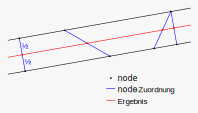
\includegraphics[width=\ScaleIfNeeded]{../chapter4/general-approach}
	\caption{Linienzusammenfassung durch Mittelpunktbildung nach Zuordnung gegenüberliegender \term{nodes}}
	\label{fig:general-approach}
}{
	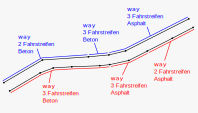
\includegraphics[width=\ScaleIfNeeded]{../chapter4/motorway-fragments}
	\caption{ungleichmäßige Fragmentierung paralleler Linienzüge (Beispiel)}
	\label{fig:motorway-fragments}
}

Um zwei gegenüberliegende \term{nodes} einander zuordnen zu können, müssen zunächst die Linien, deren Teil sie sind, als zueinander parallel erkannt werden.
Auch hierbei ist die erwähnte ungleichmäßige Fragmentierung in bestimmten Fällen problematisch.
Beispielsweise müssten die einzelnen \term{ways} in Abbildung~\ref{fig:motorway-fragments}, aus denen die beiden dargestellten Parallelen bestehen, zunächst zu einem längeren Linienzug verknüpft werden, um einen Vergleich zu ermöglichen.
Dies entspräche dem in Abschnitt~\ref{os-mastermap} beschriebenen Ansatz von Thom, der damit zufriedenstellende Resultate erzielte, dabei jedoch die hohe Qualität seiner Ausgangsdaten betonte, welche bei wie für \osm\ von Freiwilligen erfassten Geodaten nicht vorausgesetzt werden kann.
% lässt sich diese aussage belegen?

Um diese Problematik zu umgehen, verwendet das in dieser Arbeit vorgestellte Verfahren möglichst \emph{kurze} Liniensegmente anstelle möglichst \emph{langer} Linienzüge.
Die Verbindung zweier benachbarter \term{nodes} in einem \term{way} als kürzestmögliche lineare Einheit in den \osm-Ausgangsdaten (früher als \term{segment} bezeichnet \cf[57]{RT09}) ist allerdings für einen Vergleich nicht viel besser geeignet als der vollständige \term{way}%
% warum nicht? (wenig spezifisch formuliert)
, wie aus Abbildung~\ref{fig:motorway-fragments} ersichtlich ist.
% nicht wirklich gut ersichtlich; neue Abbildung mit Pfeilen wie in fig:comparable-fragments?
Daher werden die \term{segments} vor der Analyse auf Parallelität solange immer weiter unterteilt, bis schließlich ein einfacher geometrischer Vergleich möglich ist (Abbildung~\ref{fig:comparable-fragments}).

\onefigure{ht}{
	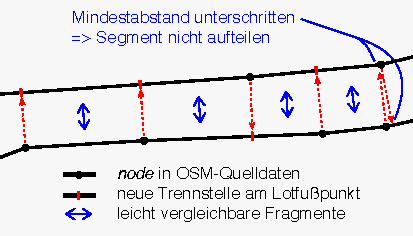
\includegraphics[width=\ScaleIfNeeded]{../chapter4/comparable-fragments}
	\caption{Herstellung einer gleichmäßigen Fragmentierung paralleler Linienzüge}
	\label{fig:comparable-fragments}
}



\section{Operationen}
\label{ch:algorithm-parts}

Der zuvor beschriebene Lösungsansatz lässt sich vereinfacht als Sequenz von vier Operationen ausdrücken:
\begin{enumerate}[nosep]
	\item Segmente unterteilen
	\item Analysieren
	\item Punktezuordnung
	\item Parallelen zusammenfassen
\end{enumerate}
%
% Datenflussdiagramm
%
Die folgenden Abschnitte beschreiben jede dieser Operationen im Detail.
Verwendete mathematische Symbole werden in Anhang~\ref{appx:mathsymbols} erklärt.

% Zur Vereinfachung Vorbedingungen der Eingabedaten: ...

% Definitionen: Ways haben Nodes; Segmente haben exakt zwei Nodes, welche mit folgender "Funktion zu erhalten sind; ...



\subsection{Segmente unterteilen}
\label{ch:split-algorithm}

In \osm-Daten sind seit Oktober~2007 Segmente (Verbindungen von exakt zwei \term{nodes}) nicht mehr als eigene Objekte enthalten \cf[57]{RT09}.
Anhand der aus der Datenquelle eingelesenen Menge aller \term{ways} wird daher zunächst durch \textproc{Segmentierung} die Menge aller Segmente ermittelt (Abbildung~\ref{fig:segments-in-way}).

\onefigure{ht}{
	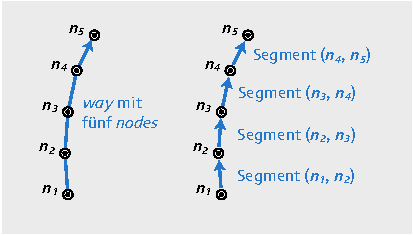
\includegraphics[width=\ScaleIfNeeded]{../chapter4/segments-in-way}
	\caption{vier Segmente in einem \term{way} (Beispiel)}
	\label{fig:segments-in-way}
}
\onefigure{!ht}{
	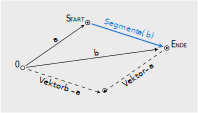
\includegraphics[width=\ScaleIfNeeded]{../chapter4/vector-geometry}
	\caption{einfache Vektorgeometrie an einem Segment demonstriert}
	\label{fig:vector-geometry}
}

Um Verbindungen zwischen zwei \term{nodes} deterministisch beschreiben zu können, werden diese hier als Kanten in einem gerichteten Graphen betrachtet.
Die beiden \term{nodes} werden als \textproc{Start} und \textproc{Ende} bezeichnet.
% evtl. besser \textproc{Ziel}, um Oberbegriff "Endpunkt" freizuhalten

Geometrisch betrachtet entsprechen \term{nodes} Punkten, die durch vom Koordinatenursprung ausgehende Vektoren in der euklidischen Ebene definiert sind.
Segmente als gerichtete Verbindungen zweier solcher Punkte lassen sich dann ebenfalls als Vektoren auffassen und als geordnetes Paar notieren.

So könnten beispielsweise die Punkte $a$ und $b$ das Segment $(a,b)$ definieren, welches geometrisch zum Vektor $b - a$ kongruent wäre (Abbildung~\ref{fig:vector-geometry}).

\begin{algorithmhere}{Segmentierung}
\label{alg:Segmentierung}
\begin{algorithmic}
\Function{Segmentierung}{$W$}\Comment{Menge aller \term{ways} $W$}
	\State $S \gets \varnothing$
	\ForAll{$w \textbf{ mit } w \in W $}
%		\State $N \gets$ alle \term{nodes} von $w$
%		\ForAll{$i \textbf{ mit } i \in \mathbb{N} : 0 < i < |N| $}\Comment{alle \term{nodes} außer dem ersten}
%			\State $n \gets$ \term{node} $i$ aus $N$
%			\State \textbf{füge} neues Segment ... \textbf{zu} $S$ \textbf{hinzu}
%		\ForAll{$n$ \textbf{mit} $n \in N \wedge \exists$ $m : m$ ist Vorgänger von $n$}
		\ForAll{$n$ \textbf{mit} $n \in w.nodes \wedge \exists\ m : m$ ist Vorgänger von $n$ in $w$}
%			\State \textbf{füge} neues Segment $(m, n)$ \textbf{zu} $S$ \textbf{hinzu}
			\State $S \gets S \cup \{(m,n)\}$\Comment{neues Segment $(m, n)$ zu $S$ hinzufügen}
		\EndFor
	\EndFor
	\State \textbf{Ergebnis} $S$
\EndFunction
\end{algorithmic}
\end{algorithmhere}
% implementiert in OsmWay.segmentation()

% "anschließend" ergibt einen etwas holprigen Übergang

Die Segmente werden anschließend durch \textproc{Splitten} derart aufgeteilt, dass ein geometrischer Vergleich leicht möglich wird (Abbildung~\ref{fig:comparable-fragments}).
Die so entstehenden Fragmente sind keine Segmente im Sinne der früheren gleichnamigen \osm-Objekte, da der Punkt, an dem sie zerteilt wurden, keinen \term{node} in OpenStreetMap darstellt.
Im Folgenden werden sie dennoch vereinfachend Segmenten gleichgestellt, da sie ansonsten dieselben Eigenschaften besitzen.

Aufgeteilt werden Segmente jeweils am \textproc{Fußpunkt} eines Lots, das von einem \term{node} eines anderen Segments gefällt wird.
Der gewählte Algorithmus für das \textproc{Splitten} arbeitet geometrisch rekursiv:
Alle erzeugten Fragmente werden wieder zur Menge der Segmente hinzugefügt und somit immer weiter aufgeteilt, bis kein \textproc{Fußpunkt} mehr gefunden wird.

% TODO: Grafik (unbedingt!), um "rekursiv" zu illustrieren

\begin{algorithmhere}{Splitten}
\label{alg:Splitten}
\begin{algorithmic}
% evtl. besser: "Assoziation" / "Relation"
\State $\textbf{Variable } wurzel : Segment \rightarrow Segment$
\State $\textbf{Anfangswert } wurzel(s) \eqdef s\;\forall\ s$
\Function{Splitten}{$S$}\Comment{Menge aller Segmente $S$}
	\State $S' \gets S$
	\ForAll{$s \textbf{ mit } s \in S'$}
		\ForAll{$n \textbf{ mit } n \in \{\textproc{Start}(s), \textproc{Ende}(s)\} $}
			\State $T \gets \textproc{NaheSegmente}(s, S')$
			\ForAll{$t \textbf{ mit } t \in T \wedge \exists\ f : f = \textproc{Fußpunkt}(n, t)$}
				\State $t_1 \gets (\textproc{Start}(t), f)$
				\State $t_2 \gets (f, \textproc{Ende}(t))$
				\State $S' \gets \{t_1, t_2\} \cup S' \setminus \{t\}$\Comment{$t$ ersetzen durch Fragmente $t_1$ und $t_2$}
				\State $wurzel(t_1) \gets wurzel(t)$
				\State $wurzel(t_2) \gets wurzel(t)$
			\EndFor
		\EndFor
	\EndFor
	\State \textbf{Ergebnis} $S'$
\EndFunction
\end{algorithmic}
\end{algorithmhere}
% implementiert in Combiner.splitSegments()

Es ist nicht notwendig, jedes Segment mit allen anderen Segmenten zu vergleichen.
Segmente, die zu weit entfernt und somit nicht \textproc{NaheSegmente} sind, können von vornherein als potenzielle Parallelen ausgeschlossen werden.
Zur Entscheidung, welche Segmente als „nah“ gelten und damit für Parallelität in Frage kommen, wird für jedes Segment eine \textproc{Hülle} gebildet, welche etwas größer als das jeweilige Segment ist, so dass sich die Hüllen von nahe beieinander liegenden Segmenten überschneiden.
% TODO: Grafik und/oder Literaturverweis

%2. Regionalisierung
%- ∀ Segmente : Liste der "nahen" anderen Segmente
%→ Spatial Index / Array (sortiert)

\begin{algorithmhere}{nahe Segmente}
\label{alg:NaheSegmente}
\begin{algorithmic}
\Function{NaheSegmente}{$s, S$}\Comment{Menge aller Segmente $S$}
	\State \textbf{Ergebnis} $\{t : t \in S \wedge \textproc{Hülle}(s) \cap \textproc{Hülle}(t) \neq \varnothing\}$
\EndFunction
\end{algorithmic}
\end{algorithmhere}
% implementiert in Combiner.regionaliseSegments()
% abweichend wird dort das Ergebnis für alle s berechnet und gecached

% TODO: Diese Definition weicht vereinfachend vom ursprünglichen Entwurf ab,
% indem alle nahen Segmente geliefert werden statt nur solche, die gleich
% ausgerichtet sind (closeSegments/closeParallels). Tests zeigen, dass diese
% Vereinfachung unzulässig ist: Das Ergebnis wird verschlechtert, weil so
% halt gerade an Kreuzungen und Querungen lauter Splits entstehen, die kein
% Mensch braucht, was die Analyse erschwert (und sicher auch ineffizient
% ist). NAHESEGMENTE muss entweder entsprechend korrigiert oder aber die
% Beschreibung entsprechend ergänzt werden. Außerdem liefert diese Definition
% fälschlich auch "s" selbst zurück, was sich allerdings durch ein einfaches
% "\wedge s \neq t" lösen lässt.

Als \textproc{Hülle} könnte ein Puffer dienen.
Aus Gründen der Effizienz bietet es sich jedoch an, die \textproc{Hülle} rechteckig im Koordinatennetz anzulegen.
Für diesen Fall hängt die Größe der Hülle auch von der Orientierung des Segments ab.
Im Ergebnis wird dann später zu sehen sein, dass diagonal zum Koordinatennetz ausgerichtete Segmente bei größeren Abständen zueinander als parallel erkannt werden als solche Segmente, die orthogonal zum Koordinatennetz ausgerichtet sind.

Um die Korrektheit der Algorithmen sicherzustellen, ist aus diesen Gründen in der späteren \textproc{Analyse} auf Parallelität eine erneute Prüfung des tatsächlichen Abstands zweier zu vergleichender Segmente notwendig.
Diese kann dann jedoch auf \textproc{NaheSegmente} beschränkt werden und ist dementsprechend billig (vergleiche Abschnitt~\ref{ch:analyse-algorithm}).

Weiterhin hängen diese Erkennungsabstände vom gewählten Koordinatennetz ab.
Würde beispielsweise mit geographischen Koordinaten gearbeitet, so variiert das Verhältnis der Erkennungsabstände in Ost/West- und in Nord/Süd-Richtung mit der geographischen Breite.
Für geometrische Operationen in der euklidischen Ebene bieten sich jedoch nur winkeltreue Abbildungen mit geringen Maßstabsfehlern im Anwendungsgebiet an. \cf[20]{Sny87}

% TODO: Grafik?

\begin{algorithmhere}{Definition der erweiterten Hüllfunktion für \textproc{NaheSegmente}}
\label{alg:Huelle}
\begin{algorithmic}
\Function{Hülle}{$s$}
	\State \textbf{Ergebnis} sei die nach allen Kardinalrichtungen um $\eta/2$ vergrößerte rechteckige Hülle um das Segment $s$, wobei $\eta$ der festzulegende Höchstabstand sei, für den zwei Segmente als „nahe“ gelten dürfen.
\EndFunction
\end{algorithmic}
\end{algorithmhere}
% implementiert in SourceSegment.envelope()

%3. Orientierungs-Ausschluss
%- ∀ Segmente : Liste der "nahen und geometrisch parallelen" Segmente

%...

%4. Splitten ("re-entrant") in Fragmente
%Liste B aller `Segment` als Basis (initial: alle `SourceSegment`)
%- _∀ B : P₁, P₂_
%    - _∀ P_ als p
%        - _∀ `splitTargets()`_ : (_target noch nicht gesplittet_ -> next;)
%            - Fußpunkt PF für p auf target suchen
%            - falls nicht außerhalb target (✐) / falls ≠ target.P₁, target.P₂: *Split* target bei PF
%                - neue Fragmente f₁, f₂ mit P₁–PF und PF–P₂ erzeugen
%                - beide f₁, f₂ an Controller melden (für Basis-Iterator: hinten anhängen an Liste zu splittender Segmente)
%                - Basis und target als gesplittet / "fertig" markieren
%                - … mehr an Controller melden…?
%(`splitTargets()`: Liste der "nahen" anderen Segmente)

\noindent
Das Aufteilen in Fragmente erfolgt jeweils am \textproc{Fußpunkt}~(Abbildung~\ref{fig:footpoint}).

\begin{algorithmhere}{Fußpunkt}
\label{alg:Fusspunkt}
\begin{algorithmic}
\Function{Fußpunkt}{$n,t$}
%	\State Es sei $l \bot t$ und $n \in l$. Dann sei $f \coloneq l \cap t$ bei $min(||f-t_1||, ||f-t_2||) > \varepsilon$ $\wedge$ $max(||f-t_1||, ||f-t_2||) < ||t||$, wobei $\varepsilon$ die festzulegende Mindestlänge eines Fragments sei.
	\State \textbf{Ergebnis} sei der Lotfußpunkt~$f$ des Punkts~$n$ auf der Geraden~$t$. Liegt~$f$ nicht zwischen den Punkten $\textproc{Start}(t)$ und $\textproc{Ende}(t)$ oder liegt~$f$ näher an $\textproc{Start}(t)$ oder $\textproc{Ende}(t)$ als die festzulegende Mindestlänge~$\mu$ eines Fragments, dann gibt es kein Ergebnis.
% Der zweite Satz ist ein wesentliches, aber nicht unbedingt offensichtliches Detail, deshalb sollte auch das an sich einfache Konzept "Lotfußpunkt" formal beschrieben werden.
\EndFunction
\end{algorithmic}
\end{algorithmhere}
% implementiert in AbstractSegment.findPerpendicularFoot()

\onefigure{H}{
	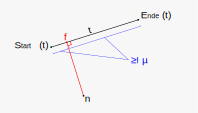
\includegraphics[width=\ScaleIfNeeded]{../chapter4/footpoint}
	\caption{Bestimmung des Punkts, an dem ein Segment aufzuteilen ist}
	\label{fig:footpoint}
}
% TODO: Abbildung verbessern: Segment s sollte enthalten sein + einheitliches Design



\subsection{Analysieren}
\label{ch:analyse-algorithm}

Das Ergebnis der Operation „Segmente unterteilen“ eignet sich zur \textproc{Analyse} auf Parallelität.
Hierfür werden Geometrie und Attribute näher verglichen mit dem Ziel, für jedes Segment beidseitig entweder genau ein oder kein anderes Segment als „parallel“ zu kennzeichnen.
% (dies funktioniert, weil bei ungleichmäßiger Fragmentierung die Verknüpfung über das _andere_ Segment hergestellt wird, d. h. dies ergibt keine 1:1-Beziehung)
%
Die Unterscheidung der Seiten links und rechts kann durch Bestimmung der Winkel zu den \term{nodes} des jeweils anderen Segments erfolgen (Abbildung~\ref{fig:left-side}).

\onefigure{ht}{
	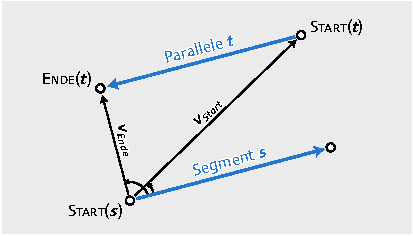
\includegraphics[width=\ScaleIfNeeded]{../chapter4/left-side}
	\caption{Erkennen einer nahen Parallele auf der linken Seite eines Segments}
	\label{fig:left-side}
}

%5. Analyse der Fragmente
%∀ Fragmente:
%- Ähnlichkeitsmaß zu allen anderen in Frage kommenden Fragmenten bestimmen (⇐ `closeParallels`), sortieren
%- aussortieren über `Analyser`
%- ∀ verbleibenden anderen Fragmente: best match(es) L+R finden, falls vorhanden (teilen 2 Segmente einen Node, ist es kein Match! (sonst klappt die L/R-Punktfindung nicht richtig)
%- best match(es) für _Segmente_ eintragen in eine Liste (und zwar reziprok) (→ eigentlich unnötig??) (∀ Segmente: ∃ 2 Listen "paralleler" Segmente) L+R (|||)

\begin{algorithmhere}{Analyse}
\label{alg:Analyse}
\begin{algorithmic}
% evtl. besser: "Assoziation" / "Relation"
\State $\textbf{Variable } parallelLinks : Segment \rightarrow Segment$
\State $\textbf{Anfangswert } parallelLinks(s) \eqdef \varnothing\ \forall\ s$
\State $\textbf{Variable } parallelRechts : Segment \rightarrow Segment$
\State $\textbf{Anfangswert } parallelRechts(s) \eqdef \varnothing\ \forall\ s$
\Function{Analyse}{$S$}\Comment{Menge aller \emph{unterteilten} Segmente $S$}
	\ForAll{$s \textbf{ mit } s \in S$}
%		\State $T \gets \{t : wurzel(t) \in \textproc{NaheSegmente}(wurzel(s), S)\} \wedge \textproc{Parallel}(s, t)$  % exakt wie implementiert, aber eigentlich in dieser Form hier nicht nötig
		\State $T \gets \{t : t \in \textproc{NaheSegmente}(s, S) \wedge \textproc{Parallel}(s, t)\}$  % vereinfachend
		\State $v_{Start} \gets \textproc{Start}(t) - \textproc{Start}(s)$
		\State $v_{Ende} \gets \textproc{Ende}(t) - \textproc{Start}(s)$
		\State $L \gets \{t : t \in T \wedge \sphericalangle (s, v_{Start}) < 0 \wedge \sphericalangle (s, v_{Ende}) < 0\}$
		\State $R \gets \{t : t \in T \wedge \sphericalangle (s, v_{Start}) > 0 \wedge \sphericalangle (s, v_{Ende}) > 0\}$
		\State\Comment{Mengen $L, R$ aller nahen Parallelen links- bzw. rechtsseitig}
		\State\Comment{Winkel seien definiert im Intervall $(-\pi,\pi)$ und im Uhrzeigersinn}
		\ForAll{$l \textbf{ mit } l \in L$}
			\If{$0 < \textproc{Distanz}(s, l) \leqslant \textproc{Distanz}(s, l')\; \forall\ l' \in L$}
				\State $parallelLinks(wurzel(s)) \gets l$
			\EndIf
		\EndFor
		\ForAll{$r \textbf{ mit } r \in R$}
			\If{$0 < \textproc{Distanz}(s, r) \leqslant \textproc{Distanz}(s, r')\; \forall\ r' \in R$}
				\State $parallelRechts(wurzel(s)) \gets r$
			\EndIf
		\EndFor
	\EndFor
	\State \textbf{Ergebnis} $parallelLinks, parallelRechts$
\EndFunction
\end{algorithmic}
\end{algorithmhere}
% implementiert in AbstractSegment.analyse()

% Die hier gewählte Definition findet für jede Seite jedes Segments höchstens ein PARALLELes Segment. Alternative wäre auch eine Definition möglich, die *jedes* PARALLELe Segment findet, weil beim NODESZUORDNEN durch die Mengeneigenschaften die Richtung der Zuordnung keine Rolle spielt und Duplikate ignoriert werden. Die Frage ist im Kern, was leichter zu verstehen ist ("parallelLinks" wäre dann eine Relation auf eine Menge von Segmenten, dafür entfiele die Prüfung ∀l' / ∀r').
% TODO: Welche Variante auch immer gewählt wird: Auf die Wahlfreiheit sollte irgendwo in 4.3 hingewiesen werden. Insbesondere falls die Implementierung von der Definition abweicht, sollte auch hierauf hingewiesen werden, z.B. in 5.4, einschließlich eines Hinweises, dass dies experimentell überprüft wurde (CorrelationGraph-realParallels-reciprocity-check).

% reicht es evtl. aus festzulegen: 2 Segmente parallel gdw. mind. je ein Fragment parallel ist? dann wäre es danach nur noch eine frage, das "beste" zu finden
% oder evtl. statt "<- l" einfach "<- wurzel(l)" und dann das als Menge ausführen? Das könnte der tatsächlichen Implementierung am ehesten entsprechen, ist aber evtl. unnötig kompliziert.

Dabei kommen nur solche Segmente für die Kennzeichnung in Frage, die im Kontext des jeweiligen Anwendungsfalls als \textproc{Parallel} gelten (vergleiche Kapitel~3).

\begin{algorithmhere}{Parallel}
\label{alg:Parallel}
\begin{algorithmic}
\Function{Parallel}{$s_1, s_2$}
	\State Die Segmente $s_1$ und $s_2$ seien parallel genau dann, wenn sie:
	\begin{itemize}[nosep,leftmargin=3.5em]
		% [SourceSegment.closeParallels]
		\item ähnlich ausgerichtet sind (z.~B. $\abs\sphericalangle (s_1, s_2)\abs < 15\degree$),
		% [MyAnalyser.shouldEvaluate]
		\item nahe beieinander liegen (z.~B. $\textproc{Distanz}(s_1, s_2) < \unit[40]{m}$),
		\item nicht so sehr zueinander versetzt sind, dass sie mehr hintereinander als nebeneinander liegen,  % "ignore collinear fragments"; sollte durch die geschickte Fragmentierung normal nicht vorkommen
		\item sich nicht überkreuzen,  % (sollte bereits durch \textproc{Analyse} ausgeschlossen sein)
		\item Teile von \term{ways} mit dem gleichen Wert für \osmtag{highway}[*] sind und
		\item Teile von \term{ways} mit dem gleichen Wert für \osmtag{ref}[*] sind.
	\end{itemize}
\EndFunction
\end{algorithmic}
\end{algorithmhere}
% implementiert in SourceSegment.closeParallels() und MyAnalyser

% Distanz 40 m:
% - vgl. https://de.wikipedia.org/wiki/Richtlinien_f%C3%BCr_die_Anlage_von_Autobahnen
% - Regelquerschnitt einer breiten Autobahn beträgt etwa 36 bis 44 m
% - theoretisch ist die Distanz die Hälfte des RQ, jedoch wird etwas Puffer benötigt, weil die Linienzüge in OSM meist nicht optimal gezeichnet sind und zudem stellenweise die Autobahnen etwas breiter als üblich gebaut sind

Dass die miteinander verglichenen Segmente nahe beieinander liegen, wird in der \textproc{Analyse} bereits durch die Beschränkung auf \textproc{NaheSegmente} sichergestellt.
Welche Segmente als „nah“ gelten, ist jedoch von der Definition der \textproc{Hülle} abhängig, für die Überlegungen zur Effizienz eine Rolle spielen (vergleiche Abschnitt~\ref{ch:split-algorithm}).
% daher in PARALLEL noch mal eine Abstands-Bedingung

% doppelt beschrieben -- was ist besser?

Aus der Menge aller als \textproc{Parallel} geltenden Segmente auf einer Seite wird das am nächsten gelegene als Parallele ausgewählt.
Auf welche Weise dazu die Distanz zwischen zwei Segmenten bestimmt wird, kann vom speziellen Anwendungsfall abhängen und soll hier nur beispielhaft angegeben werden.
So ist eine mögliche Metrik für die \textproc{Distanz} zweier Segmente der Abstand ihrer Mittelpunkte.

% tatsächlich implementiert: Summe der Abstände der jeweils nächsten Nodes (siehe MyAnalyser.evaluate)
% alternativ denkbar: _kleinster_ Abstand zweier Nodes

\begin{algorithmhere}{Beispielhafte Bestimmung der Distanz zweier Segmente}
\label{alg:Distanz}
\begin{algorithmic}
\Function{Distanz}{$s_1, s_2$}
%	\State \textbf{Ergebnis} $||\textproc{Mittelpunkt}(s_1) - \textproc{Mittelpunkt}(s_2)||$
	\State \textbf{Ergebnis} $\abs\textproc{Start}(s_1) - \textproc{Start}(s_2) + \textproc{Ende}(s_1) - \textproc{Ende}(s_2)\abs \cdot \frac{1}{2}$
\EndFunction
\end{algorithmic}
\end{algorithmhere}
% implementiert in MyAnalyser.evaluate()

%\begin{algorithm}[H]
%\caption{Mittelpunkt}\label{alg:Mittelpunkt}
%\begin{algorithmic}
%\Function{Mittelpunkt}{$s$}
%	\State \textbf{Ergebnis} $\frac{\textproc{Start}(s) + \textproc{Ende}(s)}{2}$
%\EndFunction
%\end{algorithmic}
%\end{algorithm}



\subsection{Punktezuordnung}
\label{ch:node-match-algorithm}

%7. Punktzuordnungen erzeugen (Vorstufe Generalisierung)
%
%- ∀ Segmente "S" : S hat Parallele und S noch nicht "fertig 7"
%    - ∀ Punkte (Start/End "T₁"), ∀ Seiten von S (L/R) "A"
%        - ∀ Parallelen von S "P" auf Seite A
%            - nahegelehensten Punkt finden "T₂"
%            - falls nichts gefunden (= keine Parallele auf dieser Seite), näcshtes A
%            - neue Punktzuordung: T₁ ↔︎ T₂
%    - S markieren als "fertig 7"
%
%_defer:_
%- ∀ Parallelen von S: Rekursion
%- alle Segmente/Zuordnungen für je ein ursprüngliches Segment als Teil eines "Blocks" markieren (könnte später evtl. Auffinden eines Anfangs zur Generalisierung erleichtern)

Das Zusammenfassen einander paralleler Segmente soll durch Zusammenfassen ihrer Start- und Endpunkte erfolgen.
Hierzu müssen zunächst die \term{nodes} der zusammenzufassenden Segmente einander zugeordnet werden.
% (wegen der Weiterschaltung...)
Dies geschieht auf Basis der durch die \textproc{Analyse} ermittelten Kennzeichnungen der Segmente als parallel.

Der Algorithmus \textproc{NodesZuordnen} sucht für jeden \term{node} beidseitig den jeweils am nächsten gelegenen \term{node} der als parallel gekennzeichneten Segmente (Abbildung~\ref{fig:node-matches}).

\begin{algorithmhere}{Nodes Zuordnen}
\label{alg:Zuordnen}
\begin{algorithmic}
\Function{NodesZuordnen}{$S$}
	\State $C \gets \varnothing$
	\ForAll{$s \textbf{ mit } s \in S$}
		\ForAll{$t \textbf{ mit } t \in \{parallelLinks(s), parallelRechts(s)\}$}
			\ForAll{$n_1 \textbf{ mit } n_1 \in \{\textproc{Start}(s), \textproc{Ende}(s)\} $}
				\State $n_2 \gets \begin{cases}\textproc{Start}(t) & \text{für } \abs n_1 - \textproc{Start}(t)\abs < \abs n_1 - \textproc{Ende}(t)\abs\\\textproc{Ende}(t) & \text{sonst}\end{cases}$
%				\State $C \gets \{(n_1, n_2)\} \cup C \setminus \{(n_2, n_1)\}$\Comment{entgegengesetzte Kanten ausschließen}
				\State $C \gets C \cup \{\{n_1, n_2\}\}$
			\EndFor
		\EndFor
	\EndFor
	\State \textbf{Ergebnis} $C$
\EndFunction
\end{algorithmic}
\end{algorithmhere}
% implementiert in NodeGraph.createGraph()

%Die Zuordnungen werden hier als gerichtete Kante $(n_1, n_2)$ beschrieben, obwohl die Orientierung keine Rolle spielt.
%Dies vereinfacht die weitere Verarbeitung.
%Allerdings müssen entgegengesetzte Kanten $(n_1, n_2)$ ausgeschlossen werden, um doppelte \term{nodes} im Generalisierungsergebnis zu vermeiden.

Weil die Orientierung der Zuordnungen keine Rolle spielt, wird hier mit $\{n_1, n_2\}$ ein \emph{ungeordnetes} Paar beschrieben.
Dies vermeidet Duplikate.
% Ergebnis: Abb. 29 general-approach

\onefigure{ht}{
	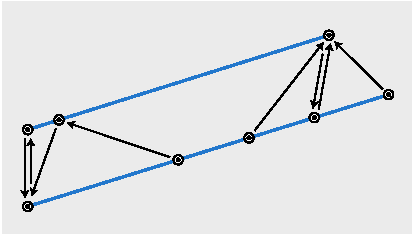
\includegraphics[width=\ScaleIfNeeded]{../chapter4/node-matches}
	\caption{Zuordnung gegenüberliegender \term{nodes} paralleler Linienzüge}
	\label{fig:node-matches}
}



\subsection{Parallelen zusammenfassen}
\label{ch:generalisation-algorithm}

%8. Generalisierung
%
%"trivialer Fall":
%1. zufällig Segment S wählen, Edge E (ES, ET) (Bedingung: Zähler E < 2)
%2. Richtung D zufällig wählen (-> S); {F,R}
%    1. gegenüberliegendes Segment T (für Start): dasjenige der beiden (<- trivialer Fall) Segment von ET, welches -- so gedreht, dass der Start-Node == ES ist -- in die gleiche Richtung zeigt wie S
%3. ∀ D :
%    1. wiederhole, solange ∃ E
%4. M-Punkt setzen
%    5. Segmente A,B von E in Richtung D: nächste Nodes N {X,Y} finden (falls ∄: N:= aktueller Node
%    6. ∀ N:
%        7. Edge F von N zurück zu E? (X->ET, Y->ES)
%           ∃: F ist nächstes E; Zähler E + 1, Zähler F + 1
%           ∄: continue 6, sonst: Edge F(X,Y)
%              ∃: F ist nächstes E
%      E=F <=> ∄: Zähler E + 1, continue 3

Anhand der Punktezuordnungen können die parallelen Segmente nun zusammengefasst werden.
Hierzu wird ein zufällig ausgewähltes Segment als Beginn eines Linienzugs betrachtet.
Während diesem Linienzug von Segment zu Segment gefolgt wird, können anhand der Punktzuordnungen leicht die Stützpunkte der Mittellinie zwischen den Parallelen als Generalisierungsergebnis bestimmt werden.

\begin{algorithmhere}{Zusammenfassen}
\label{alg:Zusammenfassen}
\begin{algorithmic}
% evtl. besser: "Assoziation" / "Relation"
\State $\textbf{Variable } zusammengefasst : Segment \rightarrow boolean$
\State $\textbf{Anfangswert } zusammengefasst(s) \eqdef$ nein $\forall\ s$
\Function{Zusammenfassen}{$S, C$}\Comment{Segmente $S$, Punktezuordnungen $C$}
	\State generalisierter Graph $\mathcal{G} \gets$ leer
	\ForAll{Segmente $s$, die noch nicht als zusammengefasst markiert sind}
		\ForAll{Zuordnungen $c$, die mit dem Start-Node $n$ von $s$ verknüpft sind}
			\State zusammengefasster Linienzug $L \gets$ leer
			\State $t \gets$ mit dem jeweils anderem Node von $c$ verknüpftes Segment,\\\qquad\qquad\qquad\quad$\hookrightarrow$ welches von $n$ aus gesehen in die gleiche Richtung zeigt wie $s$
			\While{es eine nächste Zuordnung $c'$ in dieser Richtung gibt,\\\qquad\qquad\qquad\qquad$\hookrightarrow$ die $s$ und $t$ ebenfalls einander zuordnet}
				\State $m \gets$ Mittelpunkt von $c$
				\State $m' \gets$ Mittelpunkt von $c'$
				\State füge Segment $(m, m')$ zu $L$ hinzu
				\State $s' \gets$ Segment, das $s$ nach $c'$ fortführt
				\If{$s \neq s'$}
					\State markiere $s$ als zusammengefasst
					\State $s \gets s'$
				\EndIf
				\State $t' \gets$ Segment, das $t$ nach $c'$ fortführt
				\If{$t \neq t'$}
					\State markiere $t$ als zusammengefasst
					\State $t \gets t'$
				\EndIf
				\State $c \gets c'$
			\EndWhile
			\State füge $L$ zu $\mathcal{G}$ hinzu
		\EndFor
	\EndFor
	\State füge alle nicht zusammengefassten Segmente zu $\mathcal{G}$ hinzu
	\State \textbf{Ergebnis} $\mathcal{G}$
\EndFunction
\end{algorithmic}
\end{algorithmhere}

Der Algorithmus zum \textproc{Zusammenfassen} arbeitet gierig, indem er versucht, einen möglichst langen Linienzug zu bilden.
Der Übersichtlichkeit halber berücksichtigt die hier angegebene Beschreibung jedoch nur jeweils eine Richtung vom Beginn ausgehend.
Dass bei zufällig gewähltem Beginn der zusammengefasste Linienzug meist auch in die jeweils andere Richtung verlängert werden kann, ist offensichtlich und trivial und kann leicht bei der Implementierung berücksichtigt werden.

Ebenso berücksichtigt die Beschreibung weder Kreuzungen noch den Übergang eines einzelnen Linienzugs in zwei parallele Linienzüge.

Auch der Fall von mehr als zwei Parallelen bleibt unberücksichtigt.
Dies muss bei der Implementierung bedacht werden, da der Begriff „als zusammengefasst markiert“ sonst nicht eindeutig ist.
Der hier beschriebene Algorithmus fasst $n$ parallele Linienzüge zu $n-1$ parallelen Linienzügen zusammen, die jeweils mittig zwischen zwei Parallelen in den Ausgangsdaten liegen.
Eine Erweiterung zur Zusammenfassung einer beliebigen Anzahl von Parallelen auf genau einen Linienzug ist über die Punktezuordnungen möglich, was jedoch in dieser Arbeit nicht weiter betrachtet wird.

% Weiterschaltung ist notwendig, weil ansonsten Endpunkte der generalisierten Linie nicht unbedingt aneinander anstoßen (durch Bildung von "Dreiecken" im Zuordnungsgraphen überlappen sich die Mittellinien u. U.)

% TODO: Grafik wäre hier keine schlechte Ergänzung


% Versuche mit Formelsatz
%\begin{algorithm}[H]
%\caption{Zusammenfassen}\label{alg:Zusammenfassen}
%%$\textbf{Variable } zusammengefasst : Segment \rightarrow bool$
%%\\$\textbf{Anfangswert } zusammengefasst(a) \stackrel{\text{\tiny def}}{=} nein$ $\forall$ $a$
%% \neg$ $zusammengefasst(s)
%\begin{algorithmic}
%\Function{Zusammenfassen}{$S, C$}
%	\ForAll{$s \textbf{ mit } s \in S, s =: (n_1, n_2)$}
%		\ForAll{$e \textbf{ mit } e \in C, e =: (e_1, e_2) \wedge (e_1 = n_1 \vee e_2 = n_1)$}
%			\State $T \gets \{t : t \in S, t =: (n_3, n_4) \wedge |\{e_1, e_2, n_3, n_4\}| < 4\}$
%			% T <- alle Segmente von ET
%			\ForAll{$t \textbf{ mit } t \in T, t =: (n_3, n_4)$}
%				
%				\State $ $ % hierhin jetzt die "cases" für die Drehung/Unterscheidung, damit bei 2.->1. das richtige ES/ET kommt
%			% ^--- "in die gleiche Richtung zeigt wie S" - wie ist das gemeint?
%				
%				
%			\EndFor
%		\EndFor
%	\EndFor
%	
%	
%%	\State $C \gets \varnothing$
%%	\ForAll{$s \textbf{ mit } s \in S, s =: (n_1, n_2)$}% \wedge \neg$ $fertig7(t)$}
%%		\ForAll{$t \textbf{ mit } t \in \{parallelLinks(s), parallelRechts(s)\}, t =: (n_3, n_4)$}
%%			\ForAll{$e_1 \textbf{ mit } e_1 \in \{n_1, n_2\} $}
%%				\State $e_2 \gets \begin{cases}n_3 & \text{für } ||e_1 - n_3|| \textless ||e_1 - n_4||\\n_4 & \text{sonst}\end{cases}$
%%				\State $C \gets C \cup (e_1, e_2)$\Comment{$e_2$ ist der $e_1$ am nächsten gelegene \term{node} von $t$}
%%			\EndFor
%%		\EndFor
%%%		\State $fertig7(s) \gets ja$
%%	\EndFor
%%	\State \textbf{Ergebnis} $C$
%\EndFunction
%\end{algorithmic}
%\end{algorithm}



\section{Gesamtüberblick \emph{[ausstehend]}}

\begin{algorithmhere}{Generalisierung}
\label{alg:Generalisierung}
\begin{algorithmic}
\Function{Generalisierung}{$W$}
	\State $S \gets \textproc{Segmente}(W)$
	\State $S' \gets \textproc{Splitten}(S)$\Comment{Abschnitt~\ref{ch:split-algorithm}}
	\State $\textproc{Analyse}(S')$\Comment{Abschnitt~\ref{ch:analyse-algorithm}}
	\State $C \gets \textproc{NodesZuordnen}(S)$\Comment{Abschnitt~\ref{ch:node-match-algorithm}}
	\State $\mathcal{G} \gets \textproc{Zusammenfassen}(S, C)$\Comment{Abschnitt~\ref{ch:generalisation-algorithm}}
	\State \textbf{Ergebnis} $\mathcal{G}$
\EndFunction
\end{algorithmic}
\end{algorithmhere}

Je nach Anwendungsfall sind Nachbearbeitungen und weitere Generalisierungsvorgänge sinnvoll.
In Frage kommen insbesondere die Verknüpfung von aneinander anschließenden Linienzügen sowie eine Formvereinfachung.

% TODO: Algorithmus-Eigenschaften beschreiben:
% - korrekt: nicht definiert, also nicht nachweisbar, Nachweis würde auch den Rahmen sprengen (aber anschaulich klar und später zu prüfen)
% - terminierend: ja, weil alle Schleifen auf abschließenden Mengen arbeiten, mit Ausnahme des Splittens, wobei aber durch die minimale Fragmentlänge µ eine klare Abbruchbedingung gegeben ist
% - deterministisch: nein; erstens abhängig von Input denkbar, dass je nach Reihenfolge der Iteration das Splitten und damit die Analyse unterschiedliche Ergebnisse liefert; zweitens Länge der generalisierten Linienzüge zufallsabhängig (da "rückwärts" nicht spezifiziert); jedoch nicht zu erwarten, dass diese Varianzen großen Einfluss auf das Ergebnis haben
% - Effizienz: evtl. grobe Landau-Betrachtung, bezogen auf ||W||, genaueres weiter hinten

% TODO: Analyse-Ergebnis beschreiben



%\section{alte Einteilung}
%
%\subsection{Identifikation parallel verlaufender Linien-Fragmente}
%
%Ansatz: Dieser Algorithmus eignet sich insgesamt weniger gut zur Identifikation als zur Generalisierung.
%Die Identifikation erfolgt, indem festgestellt wird, ob eine Generalisierung notwendig ist oder nicht; falls sie notwendig ist, kann sie dann aber auch bereits recht billig durchgeführt werden.
%Andererseits ist fraglich, welchen "praxistauglichen" Einsatz eine reine Identifikation ohne anschließende Generalisierung hätte.
%
%Konzept (abstrakt):
%
%1. nur Segmente betrachten (gerade Linienabschnitte, definiert durch zwei Punkte)
%
%2. alle nahe beieinander liegenden Segmente auf Parallelität untersuchen
%
%Die Segmente sind jedoch unterschiedlich lang und liegen teilweise etwas „verstreut“ im Raum, was die Untersuchung erschwert.
%Deshalb werden die Segmente zunächst fragmentiert, indem benachbarte Segmente „geschickt“ weiter in kürzere Segmente unterteilt werden, so dass parallele Segmente immer ähnlich lang sind und einander gegenüberstehen.
%
%Im Detail:
%
%1. geometrische Indizierung (R-Tree) der Eingabedaten, um Suche nach nahen Segments zu ermöglichen [regionalise]
%
%2. $\forall$ Segments: AbstractSegment.splitCloseParallels, um gut vergleichbare Stücke zu erhalten (reentrant/rekursiv, d. h. neu erzeugte Fragmente werden bis zu einer Mindestgröße immer weiter aufgeteilt) [split]
%
%3. $\forall$ Segments: $\forall$ nahe Parallelen (laut Index): [analyse]
%
%3.1 Vorprüfung (boolean)
%
%3.2 Hauptprüfung (double)
%
%3.3 best matches (links/rechts getrennt) speichern (keine Nachprüfung => falls das best match nicht passt, wird es trotzdem genommen, sofern nicht schon die vorprüfung die sache abgebrochen hat)
%% offen: "realParallels"-Konzept
%% geprüft werden die Fragmente, gespeichert werden die Segmente
%
%% graphisch erklären, was genau passiert
%
%
%\subsection{Generalisierung durch Zusammenfassung}
%
%Konzept (in den allgemeinsten Begriffen):
%
%1. Endpunkte der parallelen Segmente einander zuordnen
%
%2. Der gesamte Graph wird "durchgehangelt", indem von einem NodeMatch ausgehend immer entlang der Segmente das nächste NodeMatch gefunden wird; diese Matches werden dann durch neu erzeugte Mittelpunkte miteinander verbunden.
%
%
%
%% (Der NodeGraph ist ein Graph, in dem NodeMatches einander gegenüberliegende Knoten von parallelen Segmenten verbinden.)
%
%% new GeneralisedLines
%% - beliebigen NodeMatch auswählen und von ihr ausgehend den angrenzenden Segmenten erst in die eine, dann die andere Richtung folgen, bis das Folgen nicht mehr eindeutig möglich ist (z. B. wegen einer Abzweigung)
%% - dabei Mittelpunkte der NodeMatches jeweils einer neuen GeneralisedSection hinzufügen
%% - Segmente, die nicht zusammengefasst wurden (weil keine Parallelen existieren), werden in Sections umgewandelt und ebenfalls den GeneralisedLines hinzugefügt, um einen homogenen Ergebnisdatensatz zu erhalten
%
%...
%
%
%\subsection{Verknüpfung von Linienfragmenten zu einem einzigen kontinuierlichen Linienzug}
%
%...


% single-chapter commands
\onlyinsubfile{\listoffigures}
%\onlyinsubfile{% UTF-8

\documentclass[../main/thesis.tex]{subfiles}
\begin{document}

% include works in bibliography that aren't cited anywhere in the document (for debugging)
\onlyinsubfile{\nocite{*}}


\defbibnote{thesisBibIntro}{\justify%
Die Literaturangaben sind alphabetisch nach dem Kürzel sortiert.
Das Kürzel wird gebildet aus den ersten drei Buchstaben des Nachnamens des Autors, bei mehreren Autoren aus jeweils den Anfangsbuchstaben der Nachnamen, bei Körperschaften aus einer mnemonisch gewählten Folge von Kleinbuchstaben; jeweils ergänzt durch die letzten beiden Ziffern des Jahres der Veröffentlichung.
\par
Um ein eventuelles Nachschlagen zu erleichtern, sind die Referenzen wo immer möglich durch Angabe von Orten ergänzt, an denen eine Kopie des jeweiligen Werks am 1.~März 2018
% gegen 22~Uhr
aufzufinden war.
In der PDF-Ausgabe dieses Dokuments sind die URLs Hyperlinks.
Die Signaturen beziehen sich auf die Bibliothek des Karlsruher Instituts für Technologie und deren Standort „Fachbibliothek HsKA“.
\bigskip}


\RaggedRight
\addtocontents{toc}{\medskip}
\newpage\addcontentsline{toc}{chapter}{Literaturverzeichnis}
\printbibliography[title=Literaturverzeichnis,prenote=thesisBibIntro]

\end{document}
}
\end{document}



% TODO: Mengen besser schreiben:
% https://de.wikipedia.org/wiki/Menge_(Mathematik)#Extensionalit.C3.A4t

% UTF-8

% single-chapter commands
\documentclass[../main/thesis.tex]{subfiles}
\onlyinsubfile{\setcounter{chapter}{4}}  % single-chapter command
\begin{document}


\chapter{Implementierung}

\section{Entwicklungsumgebung}

Zur Umsetzung der entwickelten Algorithmen in Software wurde die Plattform Java verwendet.
Die Wahl von Java erfolgte neben der Vertrautheit des Verfassers mit dem zugehörigen \term{framework} aufgrund zu erwartender Effizienzvorteile von kompiliertem Code gegenüber Skriptsprachen wie Perl.
% einer Empfehlung der Geofabrik folgend

Java als imperative Sprache erlaubt es nicht, Algorithmen mit dem gleichen Grad an Abstraktion zu beschreiben wie zuvor in Kapitel~\ref{ch:algorithm-parts} geschehen.
Dort konnten zugunsten einer vereinfachten
% jedoch präzisen, cf. EWD656
Beschreibung praktische Erwägungen wie der Bedarf an Rechenzeit und Speicherplatz teilweise hintenanstehen.
Bei der Implementierung in Java müssen hingegen sorgfältig solche Datenstrukturen gewählt werden, die eine effiziente Ausführung erlauben, und die Algorithmen soweit nötig entsprechend angepasst werden.
Das Ergebnis wird in Abschnitt~\ref{ch:data-structures} beschrieben.

Während der Entwicklung wurde versucht, so viel existierenden Code in Form von \term{frameworks} wiederzuverwenden wie möglich.
Diese Bestrebung verursachte Probleme, wie auch später in Abschnitt~\ref{ch:impl-difficulties} geschildert wird.
Bei der Entwicklung kamen zuletzt die folgenden Plattformen und \term{frameworks} zum Einsatz:

\begin{itemize}[nosep]
	\item Darwin 15.6 / Mac OS X 10.11.6
	\item Java™ Standard Edition JDK 8 Update 152\\ \url{http://www.oracle.com/technetwork/java/javase/downloads/}
	\item Apache Ant 1.10.1 \quad \url{https://ant.apache.org/}
	\item args4j 2.33 \quad \url{http://args4j.kohsuke.org/}
	\item GeoTools 18.0 \quad \url{http://www.geotools.org/}
	\item TestNG 6.8 \quad \url{http://testng.org/}
	% http://web.archive.org/web/20121113133417/http://testng.org/testng-6.8.zip (all other releases appear to be corrupt; I'm probably doing something wrong)
	\item GDAL 2.2.2 \quad \url{http://www.gdal.org/}
\end{itemize}

Ursprünglich wurden ältere Softwareversionen verwendet.
Die nötigen Anpassungen an die hier genannten aktuellen Versionen waren gering, Kompatibilität mit den älteren Versionen ist jedoch gegenwärtig aufgrund von Änderungen in GeoTools nicht mehr vollständig gegeben.
Der Code ist dabei noch immer konform zum Syntax von Java 6. \cf{GJSB05}

Der folgende Abschnitt erläutert einige Überlegungen, die bei der Auswahl der \term{frameworks} relevant waren.



\section{Systemarchitektur}
\label{ch:impl-architecture}

Für ein gut funktionierendes Gesamtpaket sind vor der Umsetzung von vorgegebenen Algorithmen in ausführbarem Code einige praktische Aspekte zu bedenken.

Zunächst stellt sich die Frage nach der Benutzerschnittstelle der Software.
Die gewählte Plattform Java bietet verschiedene Möglichkeiten, graphische Benutzeroberflächen (\term{graphical user interface,} GUI) zu gestalten.
Denkbar wäre beispielsweise eine Integration in den weit verbreiteten \osm-Editor JOSM als \term{plug-in.}
Das Entwickeln und Debuggen einer GUI-Anwendung neigt jedoch dazu, zeitaufwändig zu sein.
Ohnehin würde es ein modularer Aufbau der Anwendung erlauben, zu einem späteren Zeitpunkt eine optionale GUI zu ergänzen.
\cf[171]{Muc05}
Aus diesen Gründen soll im Rahmen dieser Arbeit auf eine GUI zugunsten einer einfachen textbasierten Kommandozeilen-Schnittstelle (\term{command-line interface,} CLI) verzichtet werden.
Zum Parsen der CLI-Parameter bieten sich einfache \term{frameworks} wie etwa args4j an.

Zur Verarbeitung beliebiger Geodaten müssen diese aus Datenspeichern eingelesen und wieder ausgegeben werden können.
Um Entwicklungszeit zu sparen, sollte hierfür nach Möglichkeit ein existierendes \term{framework} genutzt werden.
Zur Vermeidung einer zu engen Kopplung der Generalisierung an das gewählte \term{framework} ist es zu vermeiden, die Primitiven des \term{frameworks} intern weiterzubenutzen.
% -> ???
Stattdessen sollten eigene Datenstrukturen genutzt werden, um Modularität zu fördern.
Die dabei entstehenden Kosten in Form von Rechenzeit und Speicherverbrauch sind zu berücksichtigen.

Da die entwickelten Algorithmen ein für das jeweilige Anwendungsgebiet optimiertes kartesisches Koordinatennetz verlangen (vgl. Abschnitt~\ref{ch:split-algorithm}), sind die aus der \osm-Datenbank stammenden Eingangsdaten nach Länge und Breite vor der Verarbeitung in einem geeigneten Kartennetzentwurf abzubilden.
Hierzu bietet sich unter anderem die UTM-Abbildung an \term{(Universal Transverse Mercator)}, welche einen querachsigen Schnittzylinder winkeltreu abbildet und zur Minimierung des Maßstabsfehlers in jeweils 6° breite Zonen unterteilt. \cf[57--58]{Sny87}
Zur Vereinfachung wird die Implementierung zunächst auf eine einzelne UTM-Zone beschränkt.

Die in Abschnitt~\ref{ch:split-algorithm} gegebene Definition für \textproc{NaheSegmente} kann leicht mit Hilfe eines R-Baums als räumlicher Index umgesetzt werden.
Die \textproc{Hülle} ist dabei das minimal umgebende Rechteck eines Blatts im R-Baum.
Nachdem die \osm-Eingangsdaten vor der Generalisierung vollständig bekannt und somit statisch sind, bietet sich der Einsatz eines gepackten R-Baums an \cf[255-256]{RSV02}.
Ein solcher Baum wird von der JTS Topology Suite (JTS) angeboten, welche vom \term{framework} GeoTools als Implementierung des Geometriemodells verwendet wird.

GeoTools bietet außerdem Möglichkeiten zur Ein- und Ausgabe (\term{input/output,} I/O) von Geodaten in zahlreichen Formaten einschließlich der Transformation von Koordinatensystemen.
Zwar wird das native \osm-XML-Format ebensowenig unterstützt wie das neuere Protocol Buffer Binary Format (PBF).
Das verbreitete Format ESRI~Shapefile wird jedoch unterstützt.
Die Geofabrik stellt aktuelle OSM-Auszüge öffentlich als Shapefile bereit.
Alternativ lassen sich Shapefiles leicht mit gängiger Software wie etwa GDAL aus anderen Formaten erzeugen.
GDAL ermöglicht dabei auch den Zuschnitt auf ein abgegrenztes Untersuchungsgebiet, was sich für Testzwecke anbietet.

\onefigure{ht}{
	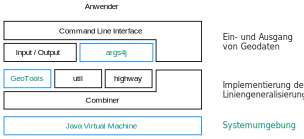
\includegraphics[width=\ScaleIfNeeded]{../chapter5/system-concept}
	\caption{Systemkonzept (schwarz: eigene Entwicklung, blau: benutztes \term{framework})}
	\label{fig:system-concept}
}

Zusammengesetzt ergibt sich aus den besprochenen Aspekten die in Abbildung~\ref{fig:system-concept} dargestellte Architektur:
Dem Anwender steht eine Kommandozeilen-Schnittstelle (CLI) zur Verfügung, die ihrerseits das \term{framework} args4j zum Parsen der Parameter sowie selbst entwickelte Routinen zur Ein- und Ausgabe der Geodaten verwendet.
Die CLI steuert damit die eigentliche Liniengeneralisierung (hier als „Combiner“ bezeichnet), welche ihrerseits neben dem \term{framework} GeoTools noch einige selbst entwickelte Hilfsmodule verwendet, die nicht vom Combiner abhängig sind und deshalb als separates Softwarepaket dargestellt werden (mit „util“ bezeichnet).
Schließlich sitzt zwischen Combiner und CLI ein mit „highway“ bezeichnetes Paket, welches versucht, die Logik des in Abschnitt~\ref{ch:case-selection} ausgewählten Spezialfalls an einem Ort zu bündeln, um die Anpassung auf andere Spezialfälle zu erleichtern.

% Noch mal Modularisierung; java Packages erwähnen/erklären? -> eher nein

Im folgenden Abschnitt wird näher auf die Implementierung der Liniengeneralisierung insbesondere im Combiner eingegangen.



\section{Datenstrukturen}
\label{ch:data-structures}

% - übergeordnete Frage: warum _so_ und nicht anders?

Aus Gründen der Übersichtlichkeit werden in den folgenden Abschnitten nur wesentliche Aspekte und wichtige Entscheidungen behandelt.
Für Detailfragen sei auf die Dokumentation der Programmierschnittstelle verwiesen, welche in englischer Sprache als Teil der Softwareentwicklung im Javadoc-Format angelegt wurde und sowohl im Java-Quellcode als auch im HTML-Format zugänglich ist.

Anhang~\ref{appx:identifiers} löst Bezeichner aus Abschnitt~\ref{ch:algorithm-parts} zu Bezeichnern im Quellcode auf.



\subsection{Grundlegendes Geometrie-Modell (GeoTools)}
\label{ch:data-structures-geotools}

Zur Umsetzung der in Abschnitt~\ref{ch:algorithm-parts} definierten geometrischen Algorithmen werden zunächst Strukturen zur Repräsentation der grundlegenden Datentypen benötigt.
Im Kontext dieses Projekts sind dies:
\begin{enumerate}[nosep]
	\item Punkt (\osm-\term{node})
	\item Segment (Verbindung von zwei Punkten als Teil eines Linienzugs)
	\item Linienzug (\osm-\term{way})
\end{enumerate}

\noindent
Das \term{framework} GeoTools benutzt dazu die JTS Topology Suite, die wie zuvor beschrieben ohnehin wegen des R-Baums für \textproc{NaheSegmente} zum Einsatz kommen soll.
JTS bietet mit der \code{Geometry}-Hierarchie Datenstrukturen nach ISO~19125\hbox{-}1 an, die grundsätzlich auch für die Implementierung der Algorithmen aus Abschnitt~\ref{ch:algorithm-parts} geeignet wären.
% http://atetric.com/atetric/javadoc/com.vividsolutions/jts-core/1.14.0/com/vividsolutions/jts/geom/package-summary.html

Die Algorithmen \textproc{Splitten} und \textproc{Analyse} ordnen den Segmenten allerdings zusätzliche Attribute zu ($wurzel$ bzw. $parallelLinks / parallelRechts$).
Dies unterstützt JTS zwar in Form von \term{user data objects}.
% http://atetric.com/atetric/javadoc/com.vividsolutions/jts-core/1.14.0/com/vividsolutions/jts/geom/Geometry.html#getUserData--
Weil jedoch die Arbeit damit eher umständlich ist, wäre dies nur sinnvoll, wenn die Nutzung der JTS-Datenstrukturen andere Vorteile bietet.

Dies ist jedoch nicht der Fall.
Im Gegenteil passen die JTS-Datenstrukturen nicht gut auf die definierten Algorithmen:
Diese beschränken sich zu einem großen Teil auf Segmente aus exakt zwei Punkten, während JTS von längeren Linienzügen ausgeht.
Die Algorithmen machen sich außerdem zunutze, dass sich Segmente direkt als Vektoren interpretieren lassen (vergleiche Abschnitt~\ref{ch:split-algorithm}).
Routinen zur Vektor-Mathematik bietet JTS zwar grundsätzlich an, jedoch sind wichtige Teile davon nicht spezifiziert.
Beispielhaft sei die Klasse \code{jts.math.Vector2D} genannt, deren Methode \code{angle()} offenbar Winkel berechnet, jedoch in keiner Weise dokumentiert ist.
% http://atetric.com/atetric/javadoc/com.vividsolutions/jts-core/1.14.0/com/vividsolutions/jts/math/Vector2D.html
Die Definition der \textproc{Analyse} auf Parallelität verlangt jedoch einen bestimmten Wertebereich für Winkel von Vektoren.
Obwohl sich die derzeitige Implementierung von \code{angle()} leicht anhand des Quellcodes von JTS ermitteln ließe, ist die Methode nicht zuverlässig verwendbar, weil ohne Dokumentation bereits unklar bleibt, ob die derzeitige Implementierung überhaupt korrekt ist.

Hinzu kommt, dass auch die von JTS angebotenen Operationen zur Manipulation geometrischer Daten -- abgesehen vom räumlichen Index -- hier wenig hilfreich sind.
Ein direktes Verwenden der bereitgestellten JTS-Datenstrukturen erscheint folglich insgesamt betrachtet nicht sinnvoll zu sein.
Stattdessen wurde ein eigenes Datenmodell entwickelt, das im Folgenden beschrieben wird.

JTS bietet die Möglichkeit, das \term{framework} zusammen mit eigenen Datenstrukturen zu benutzten, wenn diese bestimmte Schnittstellen anbieten.
% z. B. CoordinateSequence
% wie in Nr. 8 im "JTS Topology Suite Developer’s Guide" 1.4 beschrieben
Dies käme hier durchaus in Betracht, damit die eigenen Datenstrukturen zukünftig von Dritten unmittelbar mit JTS genutzt werden können.
Beispielsweise könnten so zusammengefasste Linienzüge als Ergebnisse der hier entwickelten Software direkt mit JTS einer Formvereinfachung unterzogen werden.
Weil dies jedoch nicht Bestandteil dieser Arbeit ist und ein Implementieren jener Schnittstellen keinen direkten Nutzen hat, wurde darauf zunächst verzichtet.
Es ließe sich für eine zukünftige Version leicht ergänzen.



\subsection{Grundlegendes Geometrie-Modell (eigene Entwicklung)}

Ein vollständiges Diagramm des entwickelten Datenmodells ist Anhang~\ref{appx:fullpage-model} zu entnehmen.
Vereinfacht auf die grundlegenden Geometrie-Datentypen ergibt sich das in Abbildung~\ref{fig:impl-geometry-model} gezeigte Datenmodell.
Die Segmente sind wie in Abschnitt~\ref{ch:split-algorithm} beschrieben zunächst nicht in den Eingangsdaten vorhanden; sie daraus durch \textproc{Segmentierung} herzustellen, ist jedoch nahezu trivial.

%   https://de.wikipedia.org/wiki/Assoziation_(UML)#Aggregation_und_Komposition

\onefigure{ht}{
% [Dataset]1 <>-- 0…n[Line]1 <>-- 1…n[Segment]1…n <>-- 2[Node]
	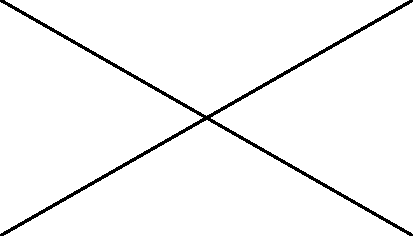
\includegraphics[width=\ScaleIfNeeded]{../image-missing}
	\\\texttt{ [Dataset]<>--[Line]<>--[Segment]<>--[Node]}
	\\\texttt{~~~~~~~~~1~~~0…n~~~1~~~1…n~~~~~1…n~~~2~~~~~}
	\caption{...}
	\label{fig:impl-geometry-model}
}

Die hier gezeigten Datentypen wurden als Interfaces (formale Schnittstellendefinitionen) umgesetzt, um ihre eventuelle Wiederverwendung zu erleichtern. \cf[18]{GHJV95}
Abbildung~\ref{fig:impl-class-structure-splitting} zeigt die bei der Implementierung dieses Datenmodells entstandene Klassenstruktur.

\onefigure{ht}{
% [Klassenstruktur "Splitten"]
	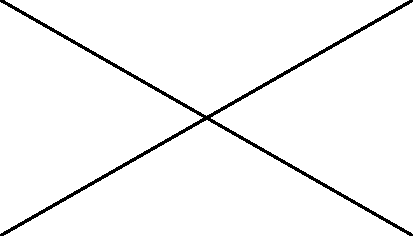
\includegraphics[width=\ScaleIfNeeded]{../image-missing}
	\caption{Klassenstruktur „Splitten“}
	\label{fig:impl-class-structure-splitting}
}

Die Anzahl der jeweils das Interface implementierenden Klassen ist in diesem Projekt klein, so dass es sich anbietet, die jeweiligen Gemeinsamkeiten in abstrakten Klassen
% wie \code{AbstractSegment}
zusammenzufassen, um Redundanzen zu vermeiden.
Diese Klassen gehören daher zu den umfangreicheren im Projekt.
% Herauszustellen ist insbesondere die Klasse \code{AbstractSegment}, welche u.~a. wichtige Algorithmen wie \textproc{Fußpunkt} und \textproc{Analyse} enthält.

Wie in Abschnitt~\ref{ch:split-algorithm} erläutert, existiert derjenige \term{node}, an dem Segmente beim \textproc{Splitten} zerteilt werden, nicht in den Eingangsdaten.
Dementsprechend wird unterschieden zwischen \code{SourceNode} (aus den \osm-Quelldaten kommend) und \code{NonexistentNode} (beim \textproc{Splitten} entstehend).
Beide implementieren jedoch die gemeinsame Schnittstelle für den Typ \code{Node}.
Zu den Gemeinsamkeiten beider Arten von \code{Node}s gehören in erster Linie deren Koordinaten, welche folglich die Klasse \code{AbstractNode} verwaltet und an die beiden konkreten Implementierungen vererbt.

In gleicher Weise fasst \code{AbstractSegment} Gemeinsamkeiten solcher Segmente, die direkt aus den Eingangsdaten stammen (\code{SourceSegment}), und solcher Segmente, die erst durch \textproc{Splitten} eines anderen Segments entstehen (\code{Fragment}), zusammen.
In Abschnitt~\ref{ch:algorithm-parts} wurden solche Segmente zur Vereinfachung einander gleichgestellt.
Für derartige Fälle schlagen Gamma et~al. den Einsatz des Kompositum-Entwurfsmusters vor:
„Use the Composite pattern when [...] you want clients to be able to ignore the difference between compositions of objects and individual objects. Clients will treat all objects in the composite structure uniformly.“ \citex[164]{GHJV95}
Im Kompositum-Muster werden Objekte zu Baumstrukturen aus individuellen Objekten (Blättern) und Komposita von Objekten zusammengefügt.

Im Kontext des Kompositum-Musters ist jedoch die Besonderheit zu berücksichtigen, dass hier einige Blätter aus den Eingangsdaten stammen (\code{SourceSegment}s), andere nicht (\code{Fragment}s).
Gleiches gilt auch für Komposita, so dass sich in einer nur auf Vererbung bestehenden Klassenstruktur sofort eine Wucherung aus größtenteils redundanten Klassen ergäbe.
Für solche Fälle schlagen Gamma et~al. vor, das Brücken-Muster \term{(Bridge pattern)} einzusetzen, mit dem die Redundanz durch Delegation vermieden werden kann. \cf[153]{GHJV95}

\onefigure{ht}{
	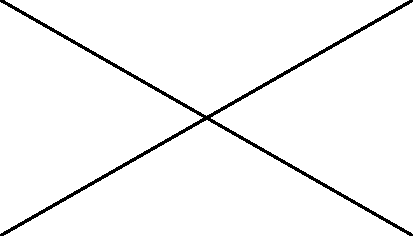
\includegraphics[width=\ScaleIfNeeded]{../image-missing}
	\caption{Composite-Bridge}
	\label{fig:impl-composite-bridge}
}

Eine Kombination aus Kompositum und Brücke wäre zwar möglich, würde jedoch zu einer recht unübersichtlichen Struktur führen.
Gamma et~al. betonen, dass Delegation unweigerlich Komplexität mit sich bringt und nur dann sinnvoll ist, wenn andere Vorteile überwiegen („Delegation is a good design choice only when it simplifies more than it complicates.“ \citex[21]{GHJV95}).
Dies wäre hier offensichtlich nicht der Fall (Abbildung~\ref{fig:impl-composite-bridge}).
Ihre Empfehlung, Delegation möglichst nur in Form von standardisierten Mustern zu verwenden, [\cfibid] scheint hier auch wegen einer weiteren Besonderheit nicht anwendbar zu sein:

Alle Objekte im \code{AbstractSegment}-Kompositum sind veränderbar (\term{mutable}), damit bei der Umwandlung von Blättern (die jeweils ein Segment repräsentieren) in Komposita (die zwei oder mehr Segmente repräsentieren) beim \textproc{Splitten} keine großen Kosten entstehen.
Bloch betont die erheblichen Vorteile von \term{immutability} (\emph{nicht} veränderbarer Objekte), weist aber auch darauf hin, dass bestimmte komplexe Operationen dann sehr teuer werden können („The performance problem is magnified if you perform a multistep operation that generates a new object at every step, eventually discarding all objects except the final result.“ \citex[67]{Blo01}).
Im vorliegenden Kompositum würde \term{immutability} gerade erfordern, dass bei jedem \textproc{Splitten} der Baum neu aufgebaut wird.

Unterschiedliche Klassen für Blätter und Komposita sind deshalb hier gar nicht angebracht; vielmehr bietet es sich \emph{in Anlehnung an} standardisierte Muster an, dass eine gemeinsame Klasse mit einem Attribut \term{children} sich entweder wie ein Blatt oder wie ein Kompositum verhält, je nachdem, ob es \term{children} in Form von Fragmenten gibt oder nicht.

\onefigure{ht}{
	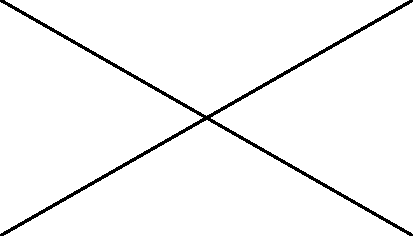
\includegraphics[width=\ScaleIfNeeded]{../image-missing}
	\caption{Composite (IST)}
	\label{fig:impl-class-structure-composite}
}

Aus dieser Erkenntnis ergibt sich eine vergleichsweise einfache Klassenstruktur (Abbildung~\ref{fig:impl-class-structure-composite}):
\code{AbstractSegment} implementiert die Gemeinsamkeiten aller Segmente.
Dazu gehört, dass jedes Segment in genau zwei Fragmente geteilt sein kann, die ihrerseits ebenfalls Segmente sind.
Jedes solche Fragment „weiß“ darüber hinaus, aus welchem Segment es abgetrennt wurde (\term{parent}).

%   [[ Textbausteine:
% In diesem speziellen Fall wird die Struktur der Komposition nur durch SPLITTEN verändert. Dabei wird genau ein Segment durch zwei andere ersetzt, die gemeinsam das ersetzte Segment repräsentieren.
% Dies entspricht zwar dem Composite-Leaf–Modell des Composite-Patterns, aber weil diese Unterscheidung orthogonal zur Unterscheidung in SourceSegment/Fragment ist, 
%   ]]

% TODO:
% soll tatsächliches Objektmodell für Fragmente gezeigt werden oder verwirrt das nur?
% wenn, dann jedenfalls besser nicht vollständig, sondern vereinfacht

Die Unterschiede zwischen \code{SourceSegment} und \code{Fragment} sind zunächst klein.
Die in Abschnitt~\ref{ch:split-algorithm} gegebene Definition von \textproc{NaheSegmente} wurde über den schon erwähnten gepackten R-Baum in JTS implementiert.
Dessen Implementierung hat den Nachteil, dass der so erzeugte R-Baum nach dem Packen nicht mehr verändert werden darf.
% [JTS docs com.vividsolutions.jts.index.strtree.STRtree] (( im Gegensatz zu der Beschreibung in [RSV02 256]! ))
Weil hier ohnehin \code{SourceSegment} als eigene Klasse existiert, bietet es sich an, die \textproc{NaheSegmente}-Logik nur in \code{SourceSegment} zu implementieren statt in der Superklasse \code{AbstractSegment}.
Das Packen des R-Baums braucht dann nur genau einmal nach dem \textproc{Segmentieren} durchgeführt zu werden.
Danach werden die \code{SourceSegment}s nicht mehr verändert.
Da Abschnitt~\ref{ch:split-algorithm} ohnehin eine erneute Abstandsprüfung in der späteren \textproc{Analyse} vorsieht, stellt diese Abweichung von der Definition der Algorithmen nicht die Korrektheit der Implementierung in Frage, obwohl sie mehr Segmente als „nah“ betrachtet als die formale Beschreibung für \textproc{NaheSegmente}.
% (weil SourceSegments obdA größer als Fragments sind). (aber NAHESEGMENTE ist ja primär eine Optimierung)

% TODO:
% Vector erwähnen!

% (weitere Besonderheiten der Konkreten ggü. Abstract*?)
%- SourceNode enthält neben der ID nur Pointers zu den Segmenten etc. für die Korralation
%- SourceSegment außerdem nur L+R sowie analyseLineParts



\subsection{Analyse und Anwendbarkeit auf andere Spezialfälle}
\label{ch:impl-analyser}

Die Algorithmen zur \textproc{Analyse} erfordern die Ergänzung des Datenmodells aus Abbildung~\ref{fig:impl-geometry-model} mit den zusätzlichen Attributen $parallelLinks$ und $parallelRechts$, in denen das Ergebnis der \textproc{Analyse} abgelegt wird.
Wie in Abschnitt~\ref{ch:algorithm-parts} definiert sind dies Attribute des Wurzel-Segments, also der Klasse \code{SourceSegment}.

Obwohl nach der Auswahl eines bestimmten Spezialfalls der Liniengeneralisierung in Abschnitt~\ref{ch:case-selection} andere Fälle nicht weiter berücksichtigt wurden, ist eine auch andere Anwendungsfälle zulassende Flexibilität doch Teil der angestrebten Praxistauglichkeit der zu entwickelnden Software.
Angesichts der Arbeitsweise der Algorithmen ist es naheliegend, dass sich dies insbesondere in der Analyse auf Parallelität niederschlagen sollte.
Die Definition der \textproc{Analyse} beschränkt sich auf geometrische Aspekte; für die konkrete Evaluierung zweiter Segmente spielen im Wesentlichen die Definitionen für \textproc{Parallel}ität und \textproc{Distanz} eine Rolle.
Es wäre daher von Vorteil, wenn diese beiden Definitionen in der Software leicht austauschbar wären.

Dieses Verhalten scheint auf den ersten Blick auf die Beschreibung des Schablonenmethoden"=Entwurfsmusters \term{(Template Method pattern)} zu passen, womit einzelne Schritte verändert werden können, ohne die gesamte Struktur eines Algorithmus zu verändern.
Tatsächlich beschränkt sich dieses Muster jedoch darauf, diese einzelnen Schritte von Unterklassen implementieren zu lassen, was auch in der einleitenden Beschreibung von Gamma et~al. schon deutlich wird:
„Template Method lets subclasses redefine certain steps of an algorithm without changing the algorithm's structure.“ \citex[325]{GHJV95}
Eine Anwendung an dieser Stelle würde also gerade unter Berücksichtigung der oben beschriebenen Komposition von Segmenten in \code{SourceSegment}s und \code{Fragment}s zu einer Wucherung von weiteren Unterklassen führen und wäre daher ungeeignet.

Stattdessen empfehlen Gamma et~al. das Besucher-Muster \term{(Visitor pattern)} einerseits gerade für solche Kompositionen, andererseits gerade dann, wenn wie hier die eigentlichen Datenstrukturen stabil sind, aber doch Flexibilität zur Definition neuer Operationen bieten sollen. \cf[333, 344]{GHJV95}
Dabei erlauben die Objekte der bereits etablierten Datentypen, ihnen einen sog. \term{visitor} als ein unabhängiges Objekt mit definierter Schnittstelle zu übergeben, welches die jeweiligen Operationen implementiert. \cf[331--335]{GHJV95}

In der vorliegenden Software akzeptieren die Segmente den Besuch eines Objekts, das die Schnittstelle \code{Analyser} implementiert.
Dieses Objekt enthält die Implementierungen der Algorithmen \textproc{Parallel} und \textproc{Distanz}.
Im Sinne der besprochenen Systemarchitektur braucht somit das Wissen über das Behandeln des in Abschnitt~\ref{ch:case-selection} gewählten Spezialfalls „baulich getrennte Richtungsfahrbahnen im Straßenraum“ nicht Teil des Combiners zu sein, sondern kann vom Client auf andere Themen angepasst werden.



\subsection{Punktezuordnung}
\label{ch:impl-node-match}

Für Abschnitt~\ref{ch:node-match-algorithm} ergibt sich das in Abbildung~\ref{fig:impl-node-match-model} gezeigte Datenmodell.
Die Klasse \code{NodeMatch} implementiert die Punktezuordnungen.
Dies sind entsprechend der formalen Definition Mengen aus exakt zwei gegenüberliegenden \term{nodes} einander paralleler Segmente.
Die Definition als mathematische Menge zur Vermeidung von Duplikaten wird später beim Zusammenfassen die Interpretation des Begriffs „nächste Zuordnung $c'$“ erleichtern (vergleiche Abschnitt~\ref{ch:generalisation-algorithm}).
Um Objekte der Klasse \code{NodeMatch} klar als Menge zu kennzeichnen, wurde sie zusätzlich als \code{Set<Node>} (Menge von \code{Node}s) im Java Collections Framework deklariert.
Dies erleichtert auch die Implementierung der Mengeneigenschaften.

\onefigure{ht}{
% [NodeGraph]1 <>-- 1…n[NodeMatch]0…n <>-- 2[Node]
	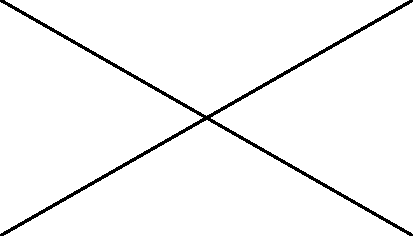
\includegraphics[width=\ScaleIfNeeded]{../image-missing}
	\\\texttt{ [NodeGraph]<>--[NodeMatch]<>--[Node]}
	\\\texttt{~~~~~~~~~~~1~~~1…n~~~~~~~0…n~~~2~~~~~}
	\caption{...}
	\label{fig:impl-node-match-model}
}

Da die \textproc{Analyse} für jedes Segment immer jeweils links- und rechtsseitig nach Parallelen sucht, werden beim \textproc{NodesZuordnen} viele Zuordnungen doppelt gefunden, nämlich einmal in jeder Richtung.
Erneut vereinfachen die Eigenschaften der mathematischen Menge, hier der Menge aller Zuordnungen $C$, die Beschreibung des Algorithmus in Abschnitt~\ref{ch:node-match-algorithm}.
Weil \code{NodeMatch}-Objekte wie beschrieben die Mengeneigenschaften implementieren, können sie leicht direkt im Java Collections Framework verwendet werden, hier als \code{Set<NodeMatch>} (Menge von \code{NodeMatch}-Objekten).
Da der Datentyp \code{NodeMatch} gleichzeitig die Schnittstelle \code{Set<Node>} implementiert, hat die Menge aller Zuordnungen implizit den Typ \code{Set<Set<Node>>}, ist also eine Menge \emph{von Mengen} von \term{nodes}, was genau der formalen Anforderung in Abschnitt~\ref{ch:node-match-algorithm} entspricht.

% TODO: SourceNode, nicht Node. Spielt das eine Rolle, oder versteht man es auch so?

Punktezuordnungen und Segmente ergeben gemeinsamen einen gemischten Graphen des zu generalisierenden Netzes.
Als parallel erkannte Segmente sind über deren \term{nodes} derart einander zugeordnet, dass sich eine gemeinsame Mittellinie als Verknüpfung der Mittelpunkte derjenigen Kanten im Graphen, welche die Punktezuordnungen darstellen, leicht finden lässt.
Zur Definition des Graphen genügt die Menge aller Punktezuordnungen, wenn über die einzelnen Punkte die mit ihnen verknüpften Segmente ermittelbar sind.

% TODO: ist hier der Fall, über addSegment(), welches in AbstractLine passiert. Sollte vielleicht weiter oben in 4.3.1 erwähnt werden. Eventuell könnte auch eine Grafik eines solchen Graphen nicht schaden.



\subsection{Liniengeneralisierung}
\label{ch:impl-generalisation}

Das Ergebnis der Liniengeneralisierung nach Abschnitt~\ref{ch:generalisation-algorithm} ist ein Graph aus Linienzügen, von denen einige durch Zusammenfassen entstehen, andere jedoch mangels Parallelen direkt aus den Eingangsdaten übernommen werden.
Der beschriebene Algorithmus zum \textproc{Zusammenfassen} ergibt einen möglichst langen Linienzug.
Um die spätere Weiterverarbeitung des Generalisierungsergebnisses zu erleichtern, werden hier auch Segmente ohne Parallele zu möglichst langen Linienzügen verkettet.

\onefigure{ht}{
% [GeneralisedLines]1 <>-- 0…n[ResultLine (Section/GeneralisedSection)]0…n <>-- 2…n[Node]
	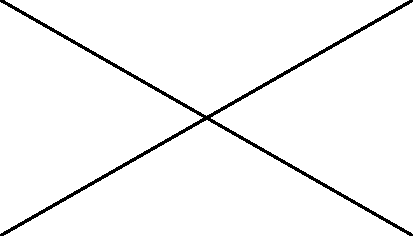
\includegraphics[width=\ScaleIfNeeded]{../image-missing}
	\\\texttt{ [GeneralisedLines]<>--[ResultLine]<>--[Node]}
	\\\texttt{~~~~~~~~~~~~~~~~~~1~~~0…n~~~~~~~~0…n~~2…n~~~~}
	\caption{...}
	\label{fig:impl-generalisation-model}
}

Entsprechend gibt es zwei unterschiedliche Arten von Linienzügen in den Ergebnisdaten.
Dies wird auch vom Datenmodell so abgebildet (Abbildung~\ref{fig:impl-generalisation-model}).
Die Klassen \code{GeneralisedSection} und \code{ConcatenatedSection} enthalten jeweils im Konstruktor Code, dem die Angabe eines geeigneten Startpunkts genügt, um einen Linienzug für das Ergebnis zu bilden.
Die bearbeiteten Segmente werden dabei entsprechend markiert, um doppelte Bearbeitungen zu vermeiden.

Die Klasse \code{GeneralisedSection} enthält den Algorithmus zum \textproc{Zusammenfassen}.
\code{ConcatenatedSection} ist ähnlich aufgebaut, aber wesentlich einfacher, da Punktezuordnungen keine Rolle spielen, sondern nur die jeweils anschließenden Segmente zu berücksichtigen sind.
Beide Klassen sind vom Typ \code{ResultLine}, um dem Client des Combiners einen einheitlichen Typ für die Ergebnisdaten liefern zu können.

Die Klasse \code{GeneralisedLines} ist eine einfache Façade für die Generalisierung, um deren Einsatz zu erleichtern.
% TODO: bessere Beschreibung + GHJV95



\subsection{Integration und ggf. Datenfluss/Interaktionswege \emph{[ausstehend]}}

\begin{itemize}
\item Integration der beschriebenen Klassen zu einem funktionierenden System
\item \code{Combiner} = Façade
\item ggf. Datenfluss/Interaktionswege
% (weichen im imperativen Code teils deutlich von funktional formulierten Algorithmen ab)
\end{itemize}



\section{Schwierigkeiten bei der Umsetzung \emph{[Entwurf]}}
\label{ch:impl-difficulties}

% TODO: "Während der Entwicklung wurde versucht, so viel existierenden Code in Form von \term{frameworks} wiederzuverwenden wie möglich. Diese Bestrebung verursachte Probleme, wie auch später in Abschnitt~\ref{ch:impl-difficulties} geschildert wird."

% TODO: commit log, Notizen und alte Screenshots/Testdaten aufarbeiten

% Wichtig: die Implementierung sollte nur dann nennenswert vom Alg. abweichen, wenn es einen Grund dafür gibt. Der muss dann auch benannt werden.
% Imperfektionen am Alg. sind aber kein Grund, ihn vor Abgabe noch zu verbessern! <= Zeitmangel



\subsection{Eigenschaften der Sprache}

\begin{itemize}

\item
Dass in den zur Verfügung stehenden Java-\term{frameworks} nicht bereits geeignete Datenstrukturen für die Arbeit mit Segmenten existieren, hat einiges an zusätzlicher Arbeit verursacht.
Das Aufbauen der Datenstrukturen war lehrreich, aber zeitaufwändiger als erwartet.

\item
Die Entwicklung von der Idee für einen Algorithmus hin zu einer für komplexe Geodaten praxistauglichen Implementierung kann als iterativer Prozess verstanden werden.
Unter dem Eindruck der Ergebnisse früher Versionen können Algorithmus und Implementierung nach und nach verfeinert werden.
% http://de.wikipedia.org/wiki/Prototyping_(Softwareentwicklung)#Evolution.C3.A4res_Prototyping
Die Wahl von Java als streng typisierte Sprache erschwerte jedoch dieses Vorgehen.
%Der Zeitaufwand dafür, elegante Klassenstrukturen aufzubauen, wurde vom Verfasser unterschätzt.

Die strenge Typisierung hat die Implementierung aufwändiger gemacht und den Fokus (bei vorgegebenem Zeitrahmen für die Arbeit) somit notwendigerweise ein Stück weit verschoben weg von Algorithmusentwicklung und -beurteilung hin zu den Details objektorientierter Programmierung.
Dies war so vor Beginn nicht absehbar.
% denn nur ich+Jochen waren Programmierer, aber nur die offiziellen Betreuer haben akad. Erfahrung
Möglicherweise wäre eine dynamisch typisierte Skriptsprache wie Perl für das explorative Vorgehen geeigneter gewesen.
% warum? -> erfordert Anpassungen der Strukturen von Algorithmen und Daten

\item
Erwartungsgemäß war das Java Collections Framework eine große Hilfe.

\item
Die Idee, nicht nur im Algorithmus, sondern auch in der Typenhierarchie Segmente als Vektoren zu behandeln, stellte sich als sehr hilfreich heraus.
Es ist denkbar, dass eine Sprache mit Operatorüberladung wie Perl diesen Vorteil noch besser hätte ausnutzen können.

\end{itemize}



\subsection{Ein- und Ausgabe von Geodaten}

\begin{itemize}

\item
Zwar ist diese Arbeit ausdrücklich aus \osm\ fokussiert, beim Prototyping stellte sich allerdings heraus, dass das direkten Einlesen von \osm-Daten etwas schwieriger war als erwartet.
Die Eingabe wurde daher zunächst über die Shapefiles der Geofabrik realisiert.
% ein spezielles Shapefile, das zusätzlich die OSM-IDs der Start- und End-Nodes enthält (nur als Debugging-Hilfe; die Algorithmen sind nicht davon abhängig)
Auch die Ausgabe erfolgt zunächst als Shapefile, damit das Generalisierungsergbnis leicht mit gängiger Software betrachtet werden kann.
Schnittstellen für Ein- und Ausgabe von \osm-Daten zu ergänzen, sollte aber nicht allzu schwierig sein.

\item
Die Shapefiles der Geofabrik enthalten aus technischen Gründen veränderte Attribute, nicht die Original-\osm-\term{tags}.
Diesem Problem wurde begegnet, indem ein Adapter die aus den Shapefiles gelesenen Attribute wieder zurück in das \osm-Format wandelt, ohne dass dies für den Combiner sichtbar wird.
% Adapter pattern: io.ShapeTagsAdapter

\item
Die Nutzung des \term{frameworks} GeoTools zur Ein- und Ausgabe von Geodaten war problematisch.
Zwar bietet GeoTools umfangreiche Unterstützung für verschiedene Datenformate, jedoch sind diese I/O-Klassen von GeoTools eher umständlich zu benutzen, ihr Interface ist nicht stabil und sie sind sehr teuer.
Eine Lösung hierfür zu entwickeln, war sehr zeitaufwändig.

Um die Datenausgabe auf eine akzeptable Geschwindigkeit zu beschleunigen, werden diese nun im GeoJSON-Format ausgegeben (implementiert als reine Textausgabe, was sehr billig ist).
Das GeoJSON wird anschließend mit GDAL in ein Shapefile konvertiert.
Insgesamt ist diese Lösung um ein Vielfaches schneller als der Shapefile-Support von GeoTools.

(Allerdings wurde der Shapefile-Support in Geotools neu implementiert; ob dies die Probleme löst, wurde noch nicht getestet.)
% http://web.archive.org/web/20130926213903/http://docs.codehaus.org/display/GEOTOOLS/Migrate+shapefile+to+shapefile-ng

\item
Außer dem eigentlichen Generalisierungsergebnis kann die entwickelte Software auch zahlreiche zusätzliche Geodatensätze ausgeben, die das Verständnis von der Arbeitsweise des Algorithmus bei Anwendung auf Real-World-Daten verbessern und auch beim Debuggen hilfreich sind.
Diese Ausgaben sind in keiner Weise optimiert.

\end{itemize}



\subsection{Sonstiges: Flexibilität und Effizienz}

\begin{itemize}

\label{ch:impl-special-case}
\item
Die Definition des Spezialfalls, auf den die Arbeit beschränkt werden soll, in einem eigenen Paket \code{highway} vom Rest des Combiners zu trennen und sie damit leicht austauschbar zu machen, war grundsätzlich eine gute Idee.
Diese Trennung ist allerdings bisher nur begonnen worden und konnte aus Zeitgründen nicht bis zum Abschluss der Arbeit beendet werden; angesichts der ausdrücklichen Beschränkung in der Aufgabenstellung auf nur den ausgewählten Spezialfall war das aber auch streng genommen gar nicht notwendig.
% betrifft insb. die Klassen Line, AbstractLine, io.InputDataset, io.ShapeReader sowie GeneralisedSection/Section
% "In der vorliegenden Software akzeptieren die Segmente den Besuch eines Objekts, das die Schnittstelle \code{Analyser} implementiert. Dieses Objekt enthält die Implementierungen der Algorithmen \textproc{Parallel} und \textproc{Distanz}." --- stimmt das überhaupt schon?

\item
Im Unterschied zur formalen Definition in Abschnitt~\ref{ch:analyse-algorithm} sind $parallelLinks$ und $parallelRechts$ nicht als homogene binäre Relation auf Segmenten implementiert, sondern als Relation zwischen Segmenten und \emph{Mengen} von Segmenten.
Mit anderen Worten: Es wird nicht jeweils nur ein einziges Segment je Seite als „parallel“ markiert, sondern mehrere.
% es wird in der Tat wie theoretisch überlegt durch die reziproke Zuordnung sichergestellt, dass auch ohne Liste für jedes Paar eine Zuordnung erstellt wird
Auf die Korrektheit der Algorithmen hat dies keinen Einfluss.
Zwar entstehen beim \textproc{NodesZuordnen} zunächst mehr Zuordnungen.
Dies sind jedoch Duplikate, die aufgrund der Mengeneigenschaft entfallen (vergleiche Abschnitt~\ref{ch:impl-node-match}).
Es stellt sich hier also die Frage, welche Implementierungsvariante mit dem Java Collections Framework am effizientesten umzusetzen ist.
Ein \term{profiling} wurde noch nicht durchgeführt.
% => Optimierungspotenzial

\item
Zahllose geschachtelte Schleifen lassen Schlimmes für die Effizienz befürchten, jedoch wird in vielen Fällen nur über eine Menge der Mächtigkeit $2$ iteriert
% (teils weniger, wie die Untersuchung zu realParallels ergab)
und in anderen Fällen wird durch \textproc{NaheSegmente} die Größe der Menge stark begrenzt; deshalb ist der Rechenaufwand in der Praxis gar nicht mal so schrecklich hoch.
Der Speicheraufwand und insbesondere das Verhalten des \term{garbage collectors} ist ein größeres Problem; hier besteht Optimierungspotenzial.

\item
Durchgehende Linienzüge sind in Kapitel~\ref{ch:algorithm-parts} spezifiziert als Mengen zusammenhängender Segmente und sind auch so in \code{AbstractLine} implementiert.
Tatsächlich müssen diese Segmente jedoch für \code{AbstractLine} in jedem Fall erst anhand einer Liste von Stützpunkten erzeugt werden.
Da für \code{ResultLine} die Segmente später ohnehin nur benötigt werden, um daraus gerade eine Liste von Stützpunkten zu erzeugen, wäre eine Optimierung von \code{AbstractLine} durch \term{lazy initialisation} angebracht:
Es würde in \code{AbstractLine} zunächst die Liste von \term{nodes} gespeichert und die \textproc{Segmentierung} erst dann durchgeführt, wenn tatsächlich Segmente angefordert werden.
% Oder es könnte evtl. auch recht einfach ResultLine einige Methoden überschreiben (coordinates, add (-> protected), get/size/iterator etc.)

\end{itemize}



% single-chapter commands
\onlyinsubfile{\listoffigures}
\onlyinsubfile{% UTF-8

\documentclass[../main/thesis.tex]{subfiles}
\begin{document}

% include works in bibliography that aren't cited anywhere in the document (for debugging)
\onlyinsubfile{\nocite{*}}


\defbibnote{thesisBibIntro}{\justify%
Die Literaturangaben sind alphabetisch nach dem Kürzel sortiert.
Das Kürzel wird gebildet aus den ersten drei Buchstaben des Nachnamens des Autors, bei mehreren Autoren aus jeweils den Anfangsbuchstaben der Nachnamen, bei Körperschaften aus einer mnemonisch gewählten Folge von Kleinbuchstaben; jeweils ergänzt durch die letzten beiden Ziffern des Jahres der Veröffentlichung.
\par
Um ein eventuelles Nachschlagen zu erleichtern, sind die Referenzen wo immer möglich durch Angabe von Orten ergänzt, an denen eine Kopie des jeweiligen Werks am 1.~März 2018
% gegen 22~Uhr
aufzufinden war.
In der PDF-Ausgabe dieses Dokuments sind die URLs Hyperlinks.
Die Signaturen beziehen sich auf die Bibliothek des Karlsruher Instituts für Technologie und deren Standort „Fachbibliothek HsKA“.
\bigskip}


\RaggedRight
\addtocontents{toc}{\medskip}
\newpage\addcontentsline{toc}{chapter}{Literaturverzeichnis}
\printbibliography[title=Literaturverzeichnis,prenote=thesisBibIntro]

\end{document}
}
\end{document}

% UTF-8

% single-chapter commands
\documentclass[../main/thesis.tex]{subfiles}
\onlyinsubfile{\setcounter{chapter}{5}}  % single-chapter command
\begin{document}


\chapter{Ergebnisdiskussion}
\label{ch:result}
% alles NUR im "Anwendungskontext", d.h. in Bezug auf die Ausgabe-Geodaten, nicht die Softwarequalität (das war in 5.4!)

%Die in Kap. 4 und 5 entwickelte Software ist das Ergebnis dieser Arbeit. Hier diskutiert werden soll die Arbeitsweise dieser Software und die Qualität der von ihr ausgegebenen Geodaten in Bezug auf die Aufgabenstellung.

Bei der Evaluierung der Software ist zu bedenken, dass die \osm-Datenbank ständig bearbeitet wird.
Konsistente Ergebnisse für ein bestimmtes Gebiet erfordern dagegen, dass immer mit Geodaten vom selben Stand gearbeitet wird.

In diesem Kapitel wird nach und nach anhand von Einzelbeispielen die Funktion der mit dieser Arbeit entwickelten Software (dem \term{Combiner}) besprochen.
Die genutzten Geodaten für das Straßennetz beschränken sich auf einen Testdatensatz aus \osm\ für das Land Nordrhein-Westfalen vom November~2012.
% http://dev.thaw.de/temp/highways/nrw-roads.zip (testbed-nrw-prepare.sh)

Anhänge~\ref{appx:fullpage-examples-1} und~\ref{appx:fullpage-examples-2} zeigen weitere Beispiele der Anwendung des \term{Combiners} auf aktuelle Geodaten größerer zusammenhängender Areale auch in anderen Regionen.



\section{Anwendung in einfachen Situationen}
\label{ch:result-trivial}

Bei Anwendung des \term{Combiners} auf Geodaten aus der \osm-Datenbank zeigt sich, dass die implementierten Algorithmen grundsätzlich funktionieren.

\onefigure{p}{
	\twofigures{H}{
		\begin{overpic}[width=\ScaleIfNeeded]{../chapter6/result-trivial-in}
			\put(122,84){\figuremark{1}}
			\put(58,60){\figuremark{2}}
			\put(23,39){\rotatebox{50}{\figureframe{.1167}}}
		\end{overpic}
	}{
		\begin{overpic}[width=\ScaleIfNeeded]{../chapter6/result-trivial-out}
			\put(122,84){\figuremark{1}}
			\put(58,60){\figuremark{2}}
			\put(23,39){\rotatebox{50}{\figureframe{.1167}}}
		\end{overpic}
	}
	% trivial = testbed-nrw/koeln-classfied-nolinks.shp
	% 1:30000 Google Mercator, bbox 778765 6607045 780865 6608245, 0.2mm stroke
	\caption{Ergebnis des \term{Combiners} im einfachen Fall (links Eingangsdaten, rechts Generalisierungsergebnis; Köln-Gremberg mit Autobahn L\,124)}
	\label{fig:result-trivial}
}

In Abbildung~\ref{fig:result-trivial} sind links \osm-Linienzüge in der einfachen Situation einer Autobahn ohne Anschlussstellen nebst innerstädtischen Sammelstraßen zu sehen.
Durch Anwendung des \term{Combiners} ergibt sich das rechts dargestellte automatisiert zusammengefasste Ergebnis.
Anstelle der beiden Richtungsfahrbahnen der Autobahn gibt es nun nur noch einen einzigen Linienzug als Straßenachse.
Die Nähe zu nachgeordneten Straßen und deren planfreie Kreuzung mit der Autobahn (bei Markierung~\textfiguremark{1}) stört die Generalisierung nicht.
Auch eine Strecke paralleler Fahrbahnen im nachgeordneten Netz wurde trotz eines scharfen Knicks erfolgreich als parallel erkannt und zusammengefasst (Markierung~\textfiguremark{2}).

\onefigure{p}{
	\twofigures{H}{
		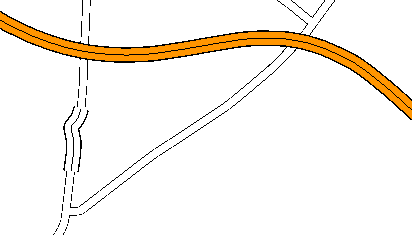
\includegraphics[width=\ScaleIfNeeded]{../chapter6/result-trivial-styled}
	}{
		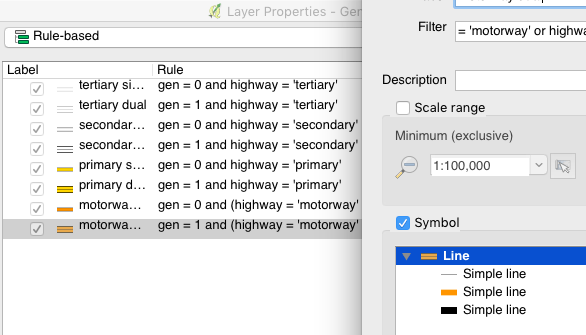
\includegraphics[width=\ScaleIfNeeded]{../chapter6/result-trivial-rules}
	}
	\caption{Visualisierung des Generalisierungsergebnisses (links Kartendarstellung, rechts Screenshot der Zeichenregeln in QGIS)}
	\label{fig:result-trivial-styled}
}

Abbildung~\ref{fig:result-trivial-styled} zeigt beispielhaft, wie sich dieses Generalisierungsergebnis sinnvoll visualisieren ließe.
Der \term{Combiner} kennzeichnet die zusammengefassten Linienzüge als generalisiert.
Zusätzlich gibt der \term{Combiner} einzelne \term{tags} der \osm-Quelldaten mit aus.
Anhand dieser Attribute können leicht Regeln mit jeweils passenden Linearsignaturen definiert werden.

% writeNodeMatches
\onefigure{p}{
	\twofigures{H}{
		\begin{overpic}[width=\ScaleIfNeeded]{../chapter6/result-trivial-detail-rolshover}
			\put(129,0){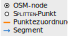
\includegraphics{../chapter6/legend-nodematch}}
			\put(53,7){\figuremark{1}}
			\put(81,85){\figuremark{2}}
			\put(184,83){\figuremark{3}}
		\end{overpic}
	}{
		\begin{overpic}[width=\ScaleIfNeeded]{../chapter6/result-trivial-detail-rolshover-gen}
			\put(129,0){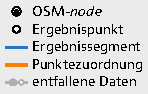
\includegraphics{../chapter6/legend-nodematch-gen}}
			\put(53,7){\figuremark{1}}
			\put(81,85){\figuremark{2}}
			\put(184,83){\figuremark{3}}
		\end{overpic}
	}
	% 1:3500 Google Mercator rotated 50°, bbox 779025 6607525 779270 6607665
	\caption{Detaildarstellung Generalisierung mit Punktezuordnungen (links Eingangsdaten, rechts Generalisierungsergebnis; \textfiguremark{2}~in Abbildung~\ref{fig:result-trivial})}
	\label{fig:result-trivial-detail-rolshover}
}

Bei näherer Betrachtung ist die korrekte Arbeitsweise der implementierten Algorithmen in diesem einfachen Fall gut zu erkennen (Abbildung~\ref{fig:result-trivial-detail-rolshover}):
Linienzüge werden durch \textproc{Splitten} derart unterteilt, dass möglichst jeweils zwei Punkte auf Parallelen einander gegenüber liegen (gut zu sehen bei~\textfiguremark{1}).
Die dabei entstehenden einander gegenüberliegenden Fragmente sind durch ihre Ähnlichkeit offensichtlich einfach auf Parallelität zu prüfen.
Selbst dann, wenn beim \textproc{Splitten} keine optimalen Paare entstehen, gelingt dies, solange wenigstens jeweils ein \emph{Teil} der miteinander verglichenen Segmente zueinander parallel ist (\textfiguremark{2}).
Von den so entstehenden Zuordnungen der einander gegenüberliegenden \osm-\term{nodes} lässt sich durch Verbindung ihrer Mittelpunkte leicht eine Mittellinie im Verlauf der Straßenachse als Ergebnis ableiten.

Der Übergang zwischen generalisierten und nicht generalisierten Linienzügen (\textfiguremark{3}) wird unten im Abschnitt~\ref{ch:relocateGeneralisedNodes} diskutiert.

Für den NRW-Testdatensatz wurden die in Abschnitt~\ref{ch:analyse-algorithm} genannten Beispielwerte von höchstens um $15\degree$ abweichender Ausrichtung und höchstens $\unit[40]{m}$ Abstand zweier \textproc{Parallel}er Segmente empirisch als grundsätzlich tauglich bestätigt.
% evtl. näher ausführen, Tabelle mit Zahlen machen, ...
Für Autobahnen genügt überwiegend bereits ein Limit von nur $10\degree$ Abweichung.
Sonstige Straßen besitzen wesentlich engere Kurvenradien und haben dabei vereinzelt Segmente, welche als parallel gelten könnten, deren Ausrichtung jedoch um $30\degree$ oder mehr voneinander abweicht.

% Ausrichtungsgrenze 15°:
% - empirisch ermittelter vernünftiger Bereich für autobahnähnlich etwa 8..16°
% - empirisch ermittelter vernünftiger Bereich für innerstädtisch etwa 20..40°

% Distanz 40 m:
% - empirisch ermittelter vernünftiger Bereich für autobahnähnlich etwa 40..45 m
% - empirisch ermittelter vernünftiger Bereich für innerstädtisch etwa 35..50 m

Um Praxistauglichkeit zu erreichen, müsste die Definition von \textproc{Parallel} folglich vom Straßentyp abhängen.
Dies wurde aus Zeitgründen nicht mehr als Teil dieser Arbeit umgesetzt.

Der NRW-Testdatensatz enthält als \osmtag{highway}[motorway] attributierte Linienzüge mit einer Gesamtlänge von $\unit[4515]{km}$.
% roads-motorway.shp
Der \term{Combiner} erkennt $\unit[4461]{km}$ davon als parallel; das ausgegebene Ergebnis besteht auf $\unit[97,6]{\%}$ Länge aus zusammengefassten Linienzügen.
Nachdem alle nordrhein-westfälischen Autobahnen zweibahnig ausgebaut sind, wäre bei naiver Betrachtung eine Erkennungsrate von $\unit[100]{\%}$ zu erwarten gewesen.
Die Untersuchung der ausgegebenen Ergebnisdaten hat gezeigt, dass Linienzüge im Wesentlichen in den folgenden Fällen als \emph{nicht} parallel erkannt werden:

\begin{itemize}[nosep]
\item fehlerhafte Klassifizierung von Auf- und Abfahrten (\osmtag{highway}[*])
% (insb. \osmtag{highway}[motorway] statt \term{motorway\_link})
\item fehlerhaftes Attribut für die Straßennummer (\osmtag{ref}[*])
% \osmtag{ref} einseitig fehlend oder voneinander abweichend
\item definierte geometrische Kriterien für Parallelität nicht erfüllt \\(z.~B. ungewöhnlich großer Abstand der Richtungsfahrbahnen)
\end{itemize}
%
Letzteres ist zu erwarten und offensichtlich korrekt.
Die ersten beiden Fälle werden in den folgenden Abschnitten~\ref{ch:result-tags} und~\ref{ch:result-junctions} näher betrachtet.



\section{Berücksichtigung von Attributen}
\label{ch:result-tags}

Die in Abschnitt~\ref{ch:analyse-algorithm} beschriebenen Algorithmen berücksichtigen neben der Klassifizierung der Straße als einziges Attribut die Straßennummer.
% in der Annahme, dass diese normalerweise stimmt
Im NRW-Testdatensatz erkennt der \term{Combiner} $\unit[54]{km}$ der Autobahn-Fahrbahnen nicht als parallel; wird die Straßennummer nicht berücksichtigt, sinkt diese Länge auf $\unit[31]{km}$.

An mehreren der dann neu erkannten Stellen trägt nur eine der beiden Richtungsfahrbahn die Straßennummer als Attribut.
In Abschnitt~\ref{ch:case-selection} wurde dargelegt, dass im Straßennetz grundsätzlich eine vergleichsweise hohe Datenqualität zu erwarten gewesen wäre, weil Fehler darin in der Standard-Karte auf \href{https://www.openstreetmap.org/}{\nolinkurl{osm.org}} störend sichtbar sind und deswegen zügig von \osm-Beitragenden behoben werden.
Die nur für \emph{eine} Richtungsfahrbahn fehlende Straßennummer fällt jedoch dem Beitragenden nicht unbedingt auf, solange die Straßennummer der \emph{anderen} Richtungsfahrbahn korrekt angezeigt wird.

Vereinzelt existieren allerdings sogar widersprüchliche Straßennummern der beiden Richtungsfahrbahnen.
So ist auf mehreren Abschnitten bei Dülmen die eine Fahrbahn \osmtag{ref}[A\,43] gekennzeichnet, die andere jedoch \osmtag{ref}[A\,43;B\,474]; bei Bliesheim trägt eine der Richtungsfahrbahnen der A\,553 das Attribut \osmtag{ref}[A\,1].

Da in diesen Fällen die Geometrie der Fahrbahnen offensichtlich parallel ist, muss hinterfragt werden, welche Bedeutung den Attributen beigemessen werden sollte.
Der \term{Combiner} berücksichtigt derzeit entgegen der ursprünglichen Definition standardmäßig nicht mehr die Straßennummer.
%Auch dies könnte jedoch zu Problemen führen, weil damit zwei Fahrbahnen gleicher Klassifizierung, die nur zufällig parallel sind, jedoch zu unterschiedlichen Straßen gehören, fälschlich als Richtungsfahrbahnen derselben Straße erkannt werden könnten.
Dieses Verhalten kann mit dem Schalter \texttt{--tags} kontrolliert werden.



\section{Verhalten an Straßenkreuzungen}
\label{ch:result-junctions}

\subsection{Beseitigung von Topologielücken}
\label{ch:relocateGeneralisedNodes}

Beim Zusammenfassen von Linienzügen erzeugt der \term{Combiner} neue Stützpunkte entlang einer Mittellinie.
Werden die Stützpunkte der ursprünglichen Linienzüge noch für weitere Zwecke verwendet, dürfen diese nicht entfallen, sondern müssen erhalten bleiben.

% [NZZ12, 14]

An \term{nodes}, die sowohl beim Zusammenfassen entfallene Linien als auch andere Linien benutzen, wird dies zum Problem:
Sie werden von nicht generalisierten Linien weiterbenutzt, die generalisierten Linien hingegen verwenden die neu erzeugten Punkte, so dass an den Übergängen topologische Lücken im Straßennetz entstehen.
Der \term{Combiner} versucht dem zu begegnen, indem die \term{nodes} an den Enden \emph{nicht} generalisierter Linienzüge auf diese Situation hin geprüft und nötigenfalls durch geeignete Punkte auf der generalisierten Mittellinie ersetzt werden.

\onefigure{h}{
	\twofigures{H}{
		\begin{overpic}[width=\ScaleIfNeeded]{../chapter6/koelnarena-gen}
			\put(0,0){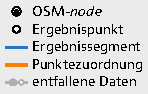
\includegraphics{../chapter6/legend-nodematch-gen}}
			\put(51,67){\figuremark{1}}
			\put(137,24){\figuremark{2}}
		\end{overpic}
	}{
		\begin{overpic}[width=\ScaleIfNeeded]{../chapter6/koelnarena-gen-cleanup}
			\put(0,0){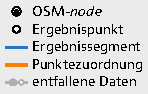
\includegraphics{../chapter6/legend-nodematch-gen}}
			\put(51,67){\figuremark{1}}
			\put(137,24){\figuremark{2}}
		\end{overpic}
	}
	% 1:5500 Google Mercator, bbox 777275 6610050 777660 6610270
	\caption{Detaildarstellung der Beseitigung von Topologielücken (links vorher, rechts nachher; L\,111 in Köln-Deutz)}
	\label{fig:koelnarena-gen-cleanup}
}

Abbildung~\ref{fig:koelnarena-gen-cleanup} zeigt, dass diese Lösung grundsätzlich funktioniert.
Die Straßenkreuzung bei \textfiguremark{1} wird auf einen einzelnen Punkt zusammengefasst, so dass beide Straßen korrekt miteinander verknüpft sind.
Auch der bereits in Abschnitt~\ref{ch:generalisation-algorithm} angesprochene und zunächst offen gelassene Übergang eines einzelnen Linienzugs in zwei parallele Linienzüge bei \textfiguremark{2} wird so gelöst.

Dieses zusätzliche, in Abschnitt~\ref{ch:algorithm-parts} nicht beschriebene Verfahren ist standardmäßig aktiv, kann aber mit dem Schalter \texttt{--no-cleanup} kontrolliert werden.
Auch in Abbildung~\ref{fig:result-trivial-detail-rolshover} kam es zum Einsatz.
Darin ist bei \textfiguremark{3} gut zu sehen, wie am Beginn des generalisierten Abschnitts die Geometrie geringfügig geändert wird, um die Topologie zu erhalten.

Topologielücken können jedoch nur dann mit diesem Verfahren geschlossen werden, wenn tatsächlich ein \emph{geeigneter} Punkt auf der generalisierten Mittellinie gefunden wird.
Wie die folgenden Abschnitte zeigen werden, ist dies oft nicht der Fall.
%Wird ein \emph{un}geeigneter Punkt gefunden, entstehen spitzwinklige Haken (siehe Anhang~\ref{appx:junction-examples}, Abbildung XYZ), Segmente mit Nulllänge usw. usf.

Mit diesem Verfahren können überdies in der gegenwärtigen Implementierung nur solche Topologielücken beseitigt werden, die erst beim Zusammenfassen von Parallelen entstanden sind.
Besonders auffallend ist diese Einschränkung bei Verbindungsrampen an planfreien Kreuzungen.
Sie sind keine Richtungsfahrbahnen und werden deshalb wie in Abschnitt~\ref{ch:case-selection} festgelegt in dieser Arbeit nicht betrachtet.
Sie sind deshalb bereits in den Eingangsdaten für die Zusammenfassung durch Objektauswahl entfallen und damit auch nicht im Generalisierungsergebnis enthalten (Abbildung~\ref{fig:breitscheid-gen-styled}).

Dass einander kreuzende Autobahnen miteinander verknüpft sind, lehrt die Lebenserfahrung; aus der Topologie der generalisierten Geodaten geht es indes nicht hervor.

\onefigure{h}{
	\begin{overpic}[width=7cm]{../chapter6/breitscheid-bg}
		\put(0,0){\scalebox{1}[1.0008]{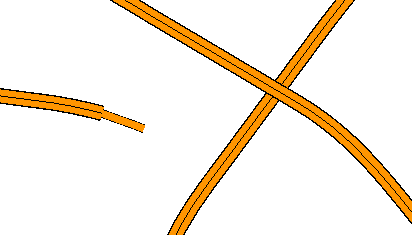
\includegraphics[width=7cm]{../chapter6/breitscheid-gen-styled}}}
	\end{overpic}
	% 1:50000 Google Mercator, bbox 761000 6682100 764500 6684100
	\caption{Fehlende Verbindungsrampen im Generalisierungsergebnis ~~~~~~~~~~~~~~~~~~~~~~~~~\cf[entsättigt][Hintergrund ]{map:osm-carto}}
	\label{fig:breitscheid-gen-styled}
}



\subsection{Fehlende Kreuzungserkennung}
\label{ch:missing-junction-detection}

\onefigure{t}{
	\begin{overpic}[width=\ScaleIfNeeded]{../chapter6/kanal-gen-cleanup}
		\put(0,67.5){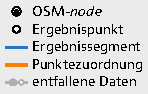
\includegraphics{../chapter6/legend-nodematch-gen}}
		\put(168,35){\figuremark{1}}
		\put(161,85){\figuremark{2}}
		\put(107,33){\figuremark{3}}
	\end{overpic}
	% 1:3500 Google Mercator rotated 10°, bbox 771595 6612098 771840 6612238
	\caption{Verbleibende Topologielücken (Innere Kanalstraße, Köln)}
	\label{fig:kanal-gen-cleanup}
}

Das in Abschnitt~\ref{ch:relocateGeneralisedNodes} beschriebene Verfahren funktioniert auch innerstädtisch nicht in jeder Situation, wie Abbildung~\ref{fig:kanal-gen-cleanup} zeigt.
Zwar führt es zu einem gelungenen Ergebnis bei \textfiguremark{1}.
Bei \textfiguremark{2} und \textfiguremark{3} wird hingegen aufgrund der spezifischen Kreuzungsgeometrie kein „geeigneter“ Punkt auf einer der generalisierten Linien gefunden.
% genauer gesagt: es werden die falschen Punkte gefunden
Die dortigen Lücken in der Topologie bleibt somit bestehen.
Ähnliche Probleme existieren an vielen weiteren innerstädtischen Kreuzungen.

Zwar ließe sich argumentieren, dass in vielen dieser Fälle die Attribute der \osm-Daten fehlerhaft sind.
Beispielsweise sollte in Abbildung~\ref{fig:kanal-gen-cleanup} die \textfiguremark{1} und \textfiguremark{3} verbindende Abbiegefahrbahn eigentlich als solche klassifiziert werden (\osmtag{highway}[primary\_link] statt \term{primary}), wodurch vermieden würde, dass sie bei \textfiguremark{3} als parallel zur Hauptfahrbahn erkannt wird. \cf{osm:HighwayLink}

Allerdings ist gerade dieser Fehler im NRW-Testdatensatz stark verbreitet.
So sind in der Kölner Innenstadt (bis einschließlich der Ringe) von insgesamt 79
% Ringe(außen) + Ringe(mittig) + Ringe(innen) + West + Nord-Süd-Fahrt + Ost:
% 6+13+15+11+26+8
Abbiegefahrbahnen ganze 26
% 2+3+6+5+9+1
nicht als solche klassifiziert.
Es ist auch fraglich, ob hier mit fortschreitender Bearbeitung der \osm-Datenbank Verbesserungen zu erwarten sind, denn Abbiegefahrbahnen und Hauptfahrbahnen werden auf \href{https://www.openstreetmap.org/}{\nolinkurl{osm.org}} mit nahezu identischer Linearsignatur gezeichnet, so dass eine falsche Klassifizierung beim Betrachten nicht auffällt.
% gemeint ist der Effekt, dass crowdgesourcte VGI im Laufe der Zeit zu Korrektheit tendiert
Vor dem Hintergrund der Aufgabenstellung, die das Ziel \emph{praxistauglicher} Algorithmen vorgibt, ist folglich offensichtlich, dass dieses Problem einer automatisierten Lösung bedarf.

An Kreisverkehren gibt es ebenfalls typische Probleme.
Abbildung~\ref{fig:roundabout-gen-cleanup} zeigt, wie alle im Kreis einander gegenüberliegenden Segmente als parallel erkannt werden.
Mit dieser Masse widersprüchlicher Punktezuordnungen kann der Algorithmus zur Zusammenfassung keine brauchbaren Ergebnisse mehr liefern.
Auch der in Abschnitt~\ref{ch:relocateGeneralisedNodes} besprochene Ansatz zur Beseitigung von Lücken in der Topologie läuft ins Leere.

\onefigure{h}{
	\begin{overpic}[width=\ScaleIfNeeded]{../chapter6/roundabout-gen-cleanup}
		\put(0,0){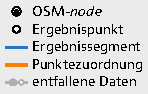
\includegraphics{../chapter6/legend-nodematch-gen}}
	\end{overpic}
	% 1:2000 Google Mercator, bbox 785968 6600972 786108 6601052
	\caption{Verhalten am Kreisverkehr (Friedrichstraße, Köln-Porz)}
	\label{fig:roundabout-gen-cleanup}
}

Zwar wäre es möglich, die meisten Kreisverkehre über \osm-\term{tags} zu erkennen und von der Generalisierung ausschließen (was aber aus Zeitgründen nicht mehr als Teil dieser Arbeit umgesetzt wurde).
% prinzipiell trivial in shouldEvaluate möglich, jedoch erfordert dies, dass die Kreisverkehr-tags vorliegen
Eine Generalisierung der Kreisverkehre -- zum~Beispiel durch Qualitätsumschlag der linearen Kreisfahrbahn in einen einzelnen Kreuzungspunkt im Zentrum -- könnte jedoch überaus nützlich sein, etwa bei der Herstellung einer Straßenkarte im mittleren Maßstabsbereich.

\newpage
Auffallend ist, dass alle diskutierten Probleme an Kreuzungen auftreten.
Auf freier Strecke funktioniert der \term{Combiner} weitgehend problemlos.
Gäbe es eine zuverlässige Methode, automatisiert Kreuzungen zu erkennen, ließe sich möglicherweise leicht Praxistauglichkeit erzielen.

Anhang~\ref{appx:junction-examples} zeigt weitere Beispiele von Kreuzungssituationen, mit denen der \term{Combiner} nicht gut zurechtkommt.



\section{Effizienz}

Die Implementierung der vorgestellten Algorithmen im \term{Combiner} hat bei Anwendung auf den NRW-Testdatensatz wie in Abschnitt~\ref{ch:algorithm-overview} erwartet einen Zeitaufwand, der im Verhältnis zur Zahl der Segmente nicht schneller als linear wächst.
Tabelle~\ref{tab:profiling-segments} stellt die gemessenen Ausführungszeiten $t$ am Beispiel von Fernstraßen (bis einschließlich \osmtag{highway}[primary], ohne \term{links}) in der Umgebung von Köln dar.
% wall clock ("processing time")
Angefangen mit einer Gruppe von Stadtteilen bis hin zum Bundesland Nordrhein-Westfalen wurden steigende Flächengrößen berechnet bei ansonsten gleichen Bedingungen.

\onetable{h}{
	\begin{tabular}{lrrlcccrc}
&&&& \multicolumn{2}{@{}c@{}}{Wachstumsfaktor} &&& \\
Gebiet & \multicolumn{1}{c}{Fläche} & \multicolumn{1}{c}{$|S|$} & \multicolumn{1}{c}{$t$} & für $|S|$ & für $t$ & $\frac{|S'|}{|S|}$ & \multicolumn{1}{c}{$\nu$} & $\psi$ \\
\hline\rule{0mm}{0.8\normalbaselineskip}%
Stadtteile &   161\,km$^2$ &   3516 & 0,41\,s & --  & --  & 1,56 & 10 & 1,31 \\
Großstadt  &   647\,km$^2$ &   8776 & 0,78\,s & 2,5 & 1,9 & 1,48 &  8 & 1,25 \\
Reg.-Bez.  &  7556\,km$^2$ &  54247 & 2,2\,s  & 6,2 & 2,8 & 1,23 &  8 & 1,37 \\
Bundesland & 34881\,km$^2$ & 157014 & 5,7\,s  & 2,9 & 2,6 & 1,27 &  6 & 1,27 \\
	\end{tabular}
	\caption{Zeitbedarf für unterschiedlich große Gebiete}
	\label{tab:profiling-segments}
}

Es bestätigt sich, dass die in Abschnitt~\ref{ch:algorithm-overview} eingeführten Größen $\nu$ und $\psi$ nicht von $|S|$ abhängig sind.
Der Wachstumsfaktor für $t$ beim Schritt von der Großstadt zum Regierungsbezirk ist mit 2,8 deutlich kleiner als der Faktor für $|S|$ mit 6,2 (also besser als für die anderen Schritte).
Wie das Verhältnis $|S'|\nobreak:\nobreak|S|$ der Segmentanzahl nach bzw. vor dem \textproc{Splitten} zeigt, liegt dies an dem mit diesem Schritt erstmals inkludierten ländlichen Raum.
Auch dies entspricht den Erwartungen.

\onetable{b}{
	\begin{tabular}{lcrcccrc}
&&& \multicolumn{2}{@{}c@{}}{Wachstumsfaktor} &&& \\
\term{links} & $|S|$ & \multicolumn{1}{c}{$t$} & für $|S|$ & für $t$ & $\frac{|S'|}{|S|}$ & \multicolumn{1}{c}{$\nu$} & $\psi$ \\
\hline\rule{0mm}{0.8\normalbaselineskip}%
ohne & 54247 & 2,2\,s  & --  & --  & 1,23 &  8 & 1,37 \\
mit & 73408 & 12,8\,s & 1,4 & 5,9 & 1,85 & 11 & 1,42 \\
	\end{tabular}
	\caption{Zeitbedarf ohne und mit Verbindungsfahrbahnen}
	\label{tab:profiling-links}
}

Wird neben der Segmentanzahl in den Eingangsdaten auch deren Detaillierungsgrad geändert, ergibt sich jedoch ein anderes Bild.
Tabelle~\ref{tab:profiling-links} zeigt das Verhalten des \term{Combiners} beim Hinzufügen von Abbiege- und Verbindungsfahrbahnen \term{(links)}.
Der Zeitbedarf wächst hier überproportional.
Dem deutlich gestiegenen Verhältnis $|S'|\nobreak:\nobreak|S|$ zufolge könnte dies an dem bereits in Abschnitt~\ref{ch:impl-special-case} angedeuteten hohen Speicheraufwand der gewählten Implementierung liegen.

Auch dies ist ein deutlicher Hinweis auf die oben diskutierte Notwendigkeit einer Kreuzungserkennung.

% durch Spectre/Meltdown keine großen Einbußen zu erwarten, weil die Berechnung hauptsächlich im RAM stattfindet und somit der Kernel keine große Rolle spielt



\section{Anwendung auf andere Spezialfälle}
\label{ch:result-other-cases}

Der nach Abschnitt~\ref{ch:case-selection} zu untersuchende Spezialfall von \emph{Richtungs}fahrbahnen impliziert, dass die entwickelten Algorithmen genau zwei entgegengerichtete Fahrbahnen derselben Straße zusammenzufassen sollen.
Ebenda wurde jedoch bereits angedeutet, dass sie möglicherweise auch auf andere Spezialfälle anwendbar sein könnten.
Abschließend soll deshalb an zwei Beispielen betrachtet werden, wie sich die im \term{Combiner} implementierten Algorithmen verhalten, wenn die Eingangsdaten nicht entsprechend dem Spezialfall aufgebaut sind, für den die Algorithmen entwickelt wurde.



\subsection{Fahrbahnen für unterschiedliche Arten von Verkehr}
%\label{ch:result-iterated-execution}

Verteilerfahrbahnen und langgezogene Rampen für abbiegenden Verkehr sind verbreitete, schon in Abschnitt~\ref{ch:different-traffic-types-case-desc} genannte Beispiele für parallele Fahrbahnen für unterschiedliche Verkehrsarten.

Nachdem der \term{Combiner} dazu vorgesehen ist, $n$~parallele Linienzüge zu $n-1$~Linienzügen zu generalisieren (mit $n=2$ im Normalfall), liegt es nahe, die Algorithmen zur Generalisierung einfach $n-1$~Mal nacheinander anzuwenden, so dass im besten Fall auch bei beliebig vielen Parallelen am Ende nur noch ein einziger Linienzug übrig bleibt.
Abbildung~\ref{fig:iteration-good} demonstriert, dass diese Strategie gelingen könnte.

\onefigure{h}{
	\twofigures{H}{
		\begin{overpic}[width=\ScaleIfNeeded]{../chapter6/opladen-gen-1}
			\put(0,0){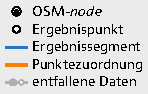
\includegraphics{../chapter6/legend-nodematch-gen}}
		\end{overpic}
	}{
		\begin{overpic}[width=\ScaleIfNeeded]{../chapter6/opladen-gen-2}
			\put(0,0){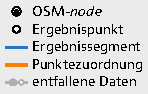
\includegraphics{../chapter6/legend-nodematch-gen}}
		\end{overpic}
	}
	% 1:6500 Google Mercator rotated -24°, bbox 778845 6630050 779300 6630310
	\caption{Detaildarstellung der wiederholten Ausführung für mehr als zwei Parallele (links erste, rechts zweite Generalisierung; A\,3 bei Leverkusen)}
	\label{fig:iteration-good}
}

Wie zu sehen ist, wird in diesem Beispiel die zwischen $2$ und $3$ variierende Zahl von Parallelen in zwei Schritten korrekt auf einen einzelnen Linienzug zusammengefasst.
Dieser liegt allerdings nicht mehr mittig im Verlauf der Straßenachse, sondern ist jeweils seitlich in Richtung der dritten Parallele verschoben.
Eine praxistaugliche Lösung müsste wie in Abschnitt~\ref{ch:generalisation-algorithm} schon angedeutet den Graphen aus Punktzuordnungen und Segmenten in seiner gesamten Breite in nur \emph{einem} Schritt beurteilen, um anhand von Attributen die tatsächliche Straßenachse ermitteln zu können.
Attribute können vom \term{Combiner} bei wiederholter Ausführung gegenwärtig nicht sinnvoll berücksichtigt werden.

Nicht unerwähnt bleiben darf, dass sich das Unvermögen des in Abschnitt~\ref{ch:relocateGeneralisedNodes} vorgestellten Ansatzes zur Beseitigung von Topologielücken, in allen Situationen einen „geeigneten“ Punkt für den Lückenschluss zu finden, bei wiederholter Ausführung besonders stark negativ auf das Ergebnis auswirkt.
Wie Abbildung~\ref{fig:iteration-gaps} zeigt, kommt es vor, dass das Generalisierungsergebnis nach mehreren Wiederholungen mit zahllosen Lücken durchsetzt ist.
Dieses Bild zeigt sich sehr verbreitet, womit das Ergebnis ungeeignet zur Weiterverarbeitung ist.

\onefigure{h}{
	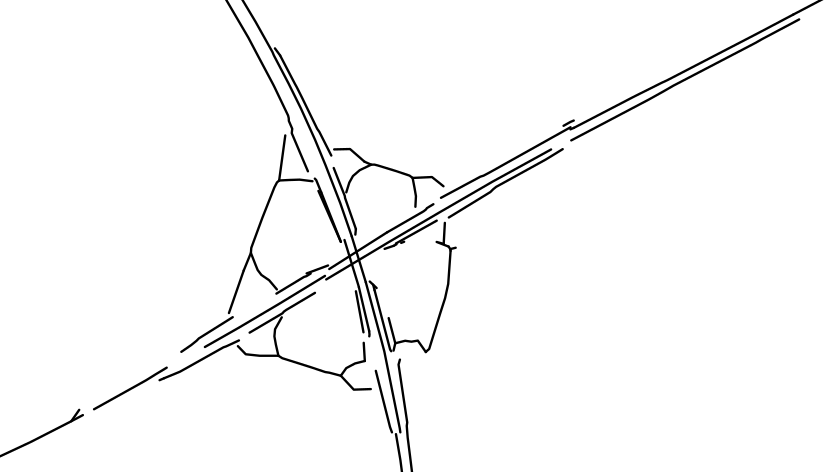
\includegraphics[width=\ScaleIfNeeded]{../chapter6/leverkusen-out}
	\caption{Überreste eines Kleeblatts nach zwei Generalisierungen (Autobahnkreuz Leverkusen)}
	\label{fig:iteration-gaps}
}

Die Anzahl der wiederholt durchzuführenden Generalisierungen kann im \term{Combiner} mit dem Schalter \texttt{--iterations} kontrolliert werden.

% evtl. beidseitig straßenbegleitende Fahrradwege zeigen (nur Erkennung)



\subsection{Eisenbahnstrecken}
\label{ch:result-railways}

Wie sich zeigt, ist die entwickelte Software grundsätzlich auch auf Eisenbahnstrecken anwendbar.
Beschränkt man sich auf Haupt- und Streckengleise (\osmtag{railway}[rail], \osmtag{usage}[main]) und berücksichtigt die Streckennummer als Attribut (\osmtag{ref}[*]), so werden viele doppelgleisige Streckenabschnitte erkannt und zusammengefasst.

Abbildung~\ref{fig:rail-kalk-out} zeigt das Ergebnis der Anwendung auf die südliche Einfahrt zum Güterbahnhof Köln-Kalk (\textfiguremark{1}).
Während die Reisezug-Gleise \textfiguremark{2}--\textfiguremark{3} und auch die drei Zulaufstrecken \textfiguremark{4}, \textfiguremark{5} und \textfiguremark{6} korrekt generalisiert wurden, funktioniert die Zuordnung im Weichenbereich bei \textfiguremark{7} nicht richtig, weil sich hier Gleise mit unterschiedlichen Streckennummern kreuzen.

Dem für ein Straßennetz entwickelten Verfahren zur Beseitigung von Topologielücken aus Abschnitt~\ref{ch:relocateGeneralisedNodes} gelingt es aufgrund der spitzen Winkel nicht, „geeignete“ Punkte zur Beseitigung der Lücken zu finden, wodurch ein gelungenes Ergebnis verhindert wird (Abbildung~\ref{fig:rail-kalk-detail}).

\onefigure{h}{
	\begin{overpic}[width=\ScaleIfNeeded]{../chapter6/rail-kalk-out}
%		\put(0,0){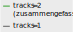
\includegraphics{../chapter6/legend-rail-out}}
	\end{overpic}
	% TODO: QGIS-export, ~10° rotiert
	\caption{Generalisierungsergebnis bei Anwendung des \term{Combiners} auf Bahnstrecken}
	\label{fig:rail-kalk-out}
}
\onefigure{h}{
	\begin{overpic}[width=\ScaleIfNeeded]{../chapter6/rail-kalk-detail}
%		\put(0,0){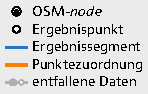
\includegraphics{../chapter6/legend-nodematch-gen}}
	\end{overpic}
	% TODO: QGIS-export, ~60° rotiert
	\caption{Detaildarstellung Generalisierung im Weichenbereich (\textfiguremark{7}~in Abbildung~\ref{fig:rail-kalk-out})}
	\label{fig:rail-kalk-detail}
}

Anders als im Straßennetz existieren derartige Probleme im Eisenbahnnetz nicht nur an Kreuzungen, sondern auch über längere Streckenabschnitte hinweg.
Betroffen sind insbesondere langgestreckte Überwerfungsbauwerke sowie Strecken mit Richtungsbetrieb.
Bei letzteren liegt zwischen den beiden zusammenzufassenden Gleisen mit derselben Streckennummer jeweils ein Gleis einer Strecke mit einer \emph{anderen} Nummer. \cf{wp:Richtungsbetrieb}

Auffallend ist ferner, dass der Zeitbedarf des \term{Combiners} für Bahnstrecken wesentlich höher ist als im Straßennetz.
Für Bahnstrecken in Köln werden mehr als 20~Segmente als „nah“ (im Sinne von \textproc{NaheSegmente} in Abschnitt~\ref{ch:split-algorithm}) beurteilt.
Dies liegt daran, dass Eisenbahngleise oft gebündelt verlegt werden, offenbar um angesichts der großen Kurvenradien den Platzbedarf zu minimieren.
Folglich sind auch entsprechend mehr Teilungen von Segmenten notwendig;
die Annahme $|S'| \approx 2 \cdot |S|$ aus Abschnitt~\ref{ch:algorithm-overview} ist selbst mit der Beschränkung auf Hauptgleise nicht mehr zutreffend.

Tabelle~\ref{tab:profiling-railways} zeigt, dass sich der Zeitbedarf durch bessere Anpassung der Definition von \textproc{Parallel} aus Abschnitt~\ref{ch:analyse-algorithm} auf die Bedingungen im Eisenbahnnetz zumindest geringfügig verbessern lässt.

\onetable{h}{
	\begin{tabular}{lrcrlcccrc}
& \multicolumn{2}{@{}c@{}}{\textproc{Parallel}} &&& \multicolumn{2}{@{}c@{}}{Wachstumsfaktor} &&& \\
Spezialfall & \multicolumn{1}{c}{$\alpha$} & $\eta$ & \multicolumn{1}{c}{$|S|$} & \multicolumn{1}{c}{$t$} & für $|S|$ & für $t$ & $\frac{|S'|}{|S|}$ & \multicolumn{1}{c}{$\nu$} & $\psi$ \\
\hline\rule{0mm}{0.8\normalbaselineskip}%
Straßen    & 15\degree & 40\,m &  8776 & 0,78\,s & --  & -- & 1,48 &  8 & 1,25 \\
Bahngleise & 15\degree & 40\,m & 11607 & 8,2\,s  & 1,3 & 11\hphantom{,2} & 2,81 & 22 & 1,77 \\
Bahngleise &  8\degree & 15\,m & 11607 & 2,5\,s  & 1,3 & \hphantom{1}3,2 & 2,14 & 11 & 1,66 \\
	\end{tabular}
	\caption{Zeitbedarf für unterschiedliche Spezialfälle und \textproc{Parallel}-Definitionen}
	\label{tab:profiling-railways}
}



% evtl. \subsection{Waldschneisen}



% single-chapter commands
\onlyinsubfile{\listoffigures}
\onlyinsubfile{\listoftables}
%\onlyinsubfile{% UTF-8

\documentclass[../main/thesis.tex]{subfiles}
\begin{document}

% include works in bibliography that aren't cited anywhere in the document (for debugging)
\onlyinsubfile{\nocite{*}}


\defbibnote{thesisBibIntro}{\justify%
Die Literaturangaben sind alphabetisch nach dem Kürzel sortiert.
Das Kürzel wird gebildet aus den ersten drei Buchstaben des Nachnamens des Autors, bei mehreren Autoren aus jeweils den Anfangsbuchstaben der Nachnamen, bei Körperschaften aus einer mnemonisch gewählten Folge von Kleinbuchstaben; jeweils ergänzt durch die letzten beiden Ziffern des Jahres der Veröffentlichung.
\par
Um ein eventuelles Nachschlagen zu erleichtern, sind die Referenzen wo immer möglich durch Angabe von Orten ergänzt, an denen eine Kopie des jeweiligen Werks am 1.~März 2018
% gegen 22~Uhr
aufzufinden war.
In der PDF-Ausgabe dieses Dokuments sind die URLs Hyperlinks.
Die Signaturen beziehen sich auf die Bibliothek des Karlsruher Instituts für Technologie und deren Standort „Fachbibliothek HsKA“.
\bigskip}


\RaggedRight
\addtocontents{toc}{\medskip}
\newpage\addcontentsline{toc}{chapter}{Literaturverzeichnis}
\printbibliography[title=Literaturverzeichnis,prenote=thesisBibIntro]

\end{document}
}
\end{document}


% TODO:
% fig:breitscheid-gen-styled - wie zentrieren und vernünftig umbrechen?
% fig:iteration-good - fehlende Punkte darstellen (als nodes, indem das Ergebnis der ersten Gen. als SHP importiert wird) und splitPts wegnehmen (bringen hier nicht mehr viel; evtl. auch Matches wegnehmen? eher ja.)
% fig:rail-kalk-out: neu
% fig:rail-kalk-detail: neu
% Legenden:
% - fig:result-trivial-detail-rolshover (rechts +splitPts, -nodes)
% - fig:koelnarena-gen-cleanup (+splitPts)
% - fig:kanal-gen-cleanup (+splitPts - oder splitPts hier schon wegnehmen? eher nicht.)
% - fig:iteration-good (unklar - erst Grafik neu)
% - fig:rail-kalk-out (fehlt)
% - fig:rail-kalk-detail (fehlt)

\chapter{Schlussfolgerung und Ausblick}

\section{Praktische Anwendbarkeit}

\begin{itemize}
	\item abschließende qualitative Gesamtbeurteilung der Arbeit auf Basis der Ergebnisuntersuchung in Bezug auf:
	\begin{itemize}
		\item Praxistauglichkeit
		\item Übertragbarkeit auf andere als die spezifizierten Spezialfälle
		\item Übertragbarkeit auf andere, ähnlich gelagerte, aber nicht identische Fragestellungen (z. B. Generalisierung durch Verdrängen)
		\item evtl. in Relation zu existierenden Lösungsansätzen (-> Analyse)
	\end{itemize}
\end{itemize}


\section{Ungelöste Problemfälle}

\begin{itemize}
	\item vorliegende Algorithmen und vorliegende Software
\end{itemize}


\section{Mögliche Ansätze zur Weiterentwicklung}

\begin{itemize}
	\item nächste Schritte
	\item neue Probleme
\end{itemize}


% Arbeit aus dem alten Standpunkt schreiben! Neuere Forschung etc. hier (und evtl. in Einleitung Kontext erklären) -DGD

% weitere Idee: Graphenanalyse: kleinste Ringe finden und prüfen, ob der umschlossene Raum eine ausreichend schmale und lange Form hat, um als parallel gelten zu können; Kreuzungen erkennen durch Mindestgröße (falls unterschritten, auf einen einzigen node zusammenfassen) [ähnlich Tho05]

% UTF-8

% single-chapter commands
\documentclass[../main/thesis.tex]{subfiles}
\onlyinsubfile{\setcounter{chapter}{7}}  % single-chapter command
\begin{document}


\chapter{Zusammenfassung}

Das Projekt OpenStreetMap (OSM) hat das Ziel der Erstellung einer freien Geodatenbank auf Basis von \term{volunteered geographic information} (VGI).
Die weitere Verarbeitung und Visualisierung von \osm-Daten läuft in aller Regel voll automatisiert ab.
Sie wird erschwert durch den teilweise sehr hohen Detailreichtum, die daraus folgende Fragmentierung von Linienzügen sowie unvollständige Verknüpfungen zusammenhängender Geodaten wie etwa parallelen Richtungsfahrbahnen über Relationen im Datenmodell.

Eine kartographische Generalisierung von \osm-Daten findet bisher nur in geringstem Umfang statt.
Dies fällt unter anderem bei parallelen Richtungsfahrbahnen auf, deren Straßenachse in \osm\ nicht erfasst ist und bisher auch nicht in zufriedenstellender Weise automatisiert abgeleitet werden kann.
%Hier kommt es verbreitet zu unbefriedigenden Darstellungen wie etwa dem Unterschreiten kartographischer Mindestgrößen sowie Fehlern wie etwa dem Überkreuzen der beiden Richtungsfahrbahnen bei Formvereinfachung.
Ansätze zur automatisierten Zusammenfassung von Linienzügen existieren, sind jedoch auf \osm-Daten nicht gut anwendbar.
Insbesondere können sie Kreuzungssituationen oft nicht ohne besondere Attribute lösen.

Diese Arbeit stellt eine Methode zur Erkennung paralleler Linienzüge auf der Basis eines geometrischen Vergleichs kurzer Fragmente vor.
Linienzüge aus \osm\ werden so lange unterteilt, bis sich Stützpunkte auf Parallelen derart einander gegenüberliegen, dass eine Prüfung auf Parallelität leicht möglich ist.
Die anschließende Zusammenfassung der erkannten Parallelen ist dann einfach zu lösen.
Der Rechenaufwand der entwickelten Algorithmen wächst linear mit der Anzahl der Stützpunkte ($\mathcal{O}(n)$).
% eigentlich linear zur Anzahl der Segmente, aber deren Zahl ist proportional zur Anzahl der Stützpunkte, so dass dies keinen Unterschied macht

Zum Nachweis ihrer Funktionsfähigkeit und zum Test mit \term{real world}--Daten aus \osm\ erfolgte ihre ausführbare Implementierung.
Aufgrund einiger technischer Schwierigkeiten war dies aufwändiger als erwartet.
% was den Fokus ein Stück weit weg von der Kartographie hin zur Informatik verschob
Die mit Java entwickelte Software („Combiner“) hat erhebliches Optimierungspotenzial.

Wie sich zeigt, führt die mit dieser Arbeit entwickelte Methode in vielen Fällen zu einem guten Generalisierungsergebnis.
Jedoch leidet auch diese Methode an erheblichen Problemen in Kreuzungssituationen.
Aus Zeitgründen war es nicht möglich, eine praxistaugliche Lösung für diese Probleme zu finden.

% Attribute könnten hier noch erwähnt werden ... sie waren zwar bisher kein großer Teil der Arbeit, müssten es aber werden, wenn Praxistauglichkeit erreicht werden soll

Auch für andere, parallel entwickelte Methoden neueren Datums wird von ähnlichen Problemen in Kreuzungssituationen berichtet.
Eine offensichtliche Lösung mit allgemeiner Anwendbarkeit für das Problem der Zusammenfassung paralleler Linienzüge zeichnet sich derzeit nicht ab.
Es ist jedoch anzunehmen, dass eine zuverlässige automatisierte Kreuzungserkennung die Zusammenfassung zu einem leicht lösbaren Problem machen würde.
Diese Arbeit benennt dazu mehrere unterschiedliche mögliche Ansätze.



\chapter*{Summary}
\addcontentsline{toc}{chapter}{Summary}

...



% single-chapter commands
\end{document}


\nocite{*}  % include works in bibliography that aren't cited anywhere in the document (for debugging)
\setbibpreamble{Die Literaturangaben sind alphabetisch nach den Nachnamen der Autoren sortiert. Bei mehreren Autoren wird nach dem ersten Autor sortiert.\par\bigskip\bigskip}
\bibliographystyle{myAMSalpha}
\bibliography{thesis}{}

%\appendix
%\chapter{Glossar}
%\chapter{Abkürzungsverzeichnis}
%\chapter{Software-Dokumentation}

\end{document}
